\chapter{Auswertung zur \tit{Kaiserchronik}}
\label{ch:kcanalyse}

Wie im Analysekapitel zum \citetitle*{cao} (\citetitle{cao}) werden im
Folgenden zunächst die gesammelten Belege dialektgeografisch eingeordnet.
Danach folgt die Untersuchung der Verteilung der Formen des Quantors
\norm{bėide} in Bezug auf die unterschiedlichen morphosyntaktischen Kontexte,
in denen er belegt ist. Zunächst sollen diejenigen Kontexte beleuchtet werden,
in denen \norm{bėide} von Substantiven sowie Pronomina abhängt und deren
Personenmerkmale durch Kongruenz reflektiert. In einem zweiten Teil wird nach
möglichen Effekten der Distanz zwischen Controller und Target gefragt. Der
dritte Abschnitt schließt dieses Kapitel mit einer Untersuchung von
\norm{bėide} als Konjunktion in Anlehnung an die Untersuchungen von
\citet{askedal1974,gjelsten1980} ab. Wie zuvor wird jeweils ein tabellarischer
Überblick über die Belegverteilung gegeben. Einzelfälle, Ausnahmen und
Zweifelsfälle werden exemplarisch diskutiert. Da die \citetitle{kc}
(\citet{kc}) in einer Vielzahl von Handschriften überliefert ist, werden dabei
wenn möglich relevante Parallelbelege hinzugezogen.

\section{Verteilung der gesammelten Belege in Zeit und Raum}
\label{subsec:beiddispmap}

Die Karte in \cref{fig:kartebelegzahl} zeigt die Menge der pro Handschrift
exzerpierten Belege für mhd.\ \norm{bėide} pro Ort beziehungsweise Gebiet. Dabei
sticht besonders das bairische Sprachgebiet heraus. Dies ist dem Umstand
geschuldet, dass die \citet{kc} vor allem im bairisch-österreichischen Raum
überliefert ist \autocite{klein1988}. Dezidiert alemannische Textzeugen, die
sich unter geografischen Gesichtspunkten mehr oder weniger direkt mit dem
Großteil der Urkundenbelege vergleichen ließen, sind abgesehen von \citet{kc:K}
(mittelalemannisch) nur unter den Fragmenten zu finden, die bei der
vorliegenden Arbeit nicht berücksichtigt wurden.%
%
	\footnote{Die Liste der Handschriftensiglen befindet sich im
		Literaturverzeichnis und richtet sich nach \citetitle{kcdigital} unter
		\urlcite{kcdigital}. \citet{kc}-Versnummern richten sich nach der
		Ausgabe von \nosh\citet{schroeder1895}.%
	}

\begin{figure}
\centering
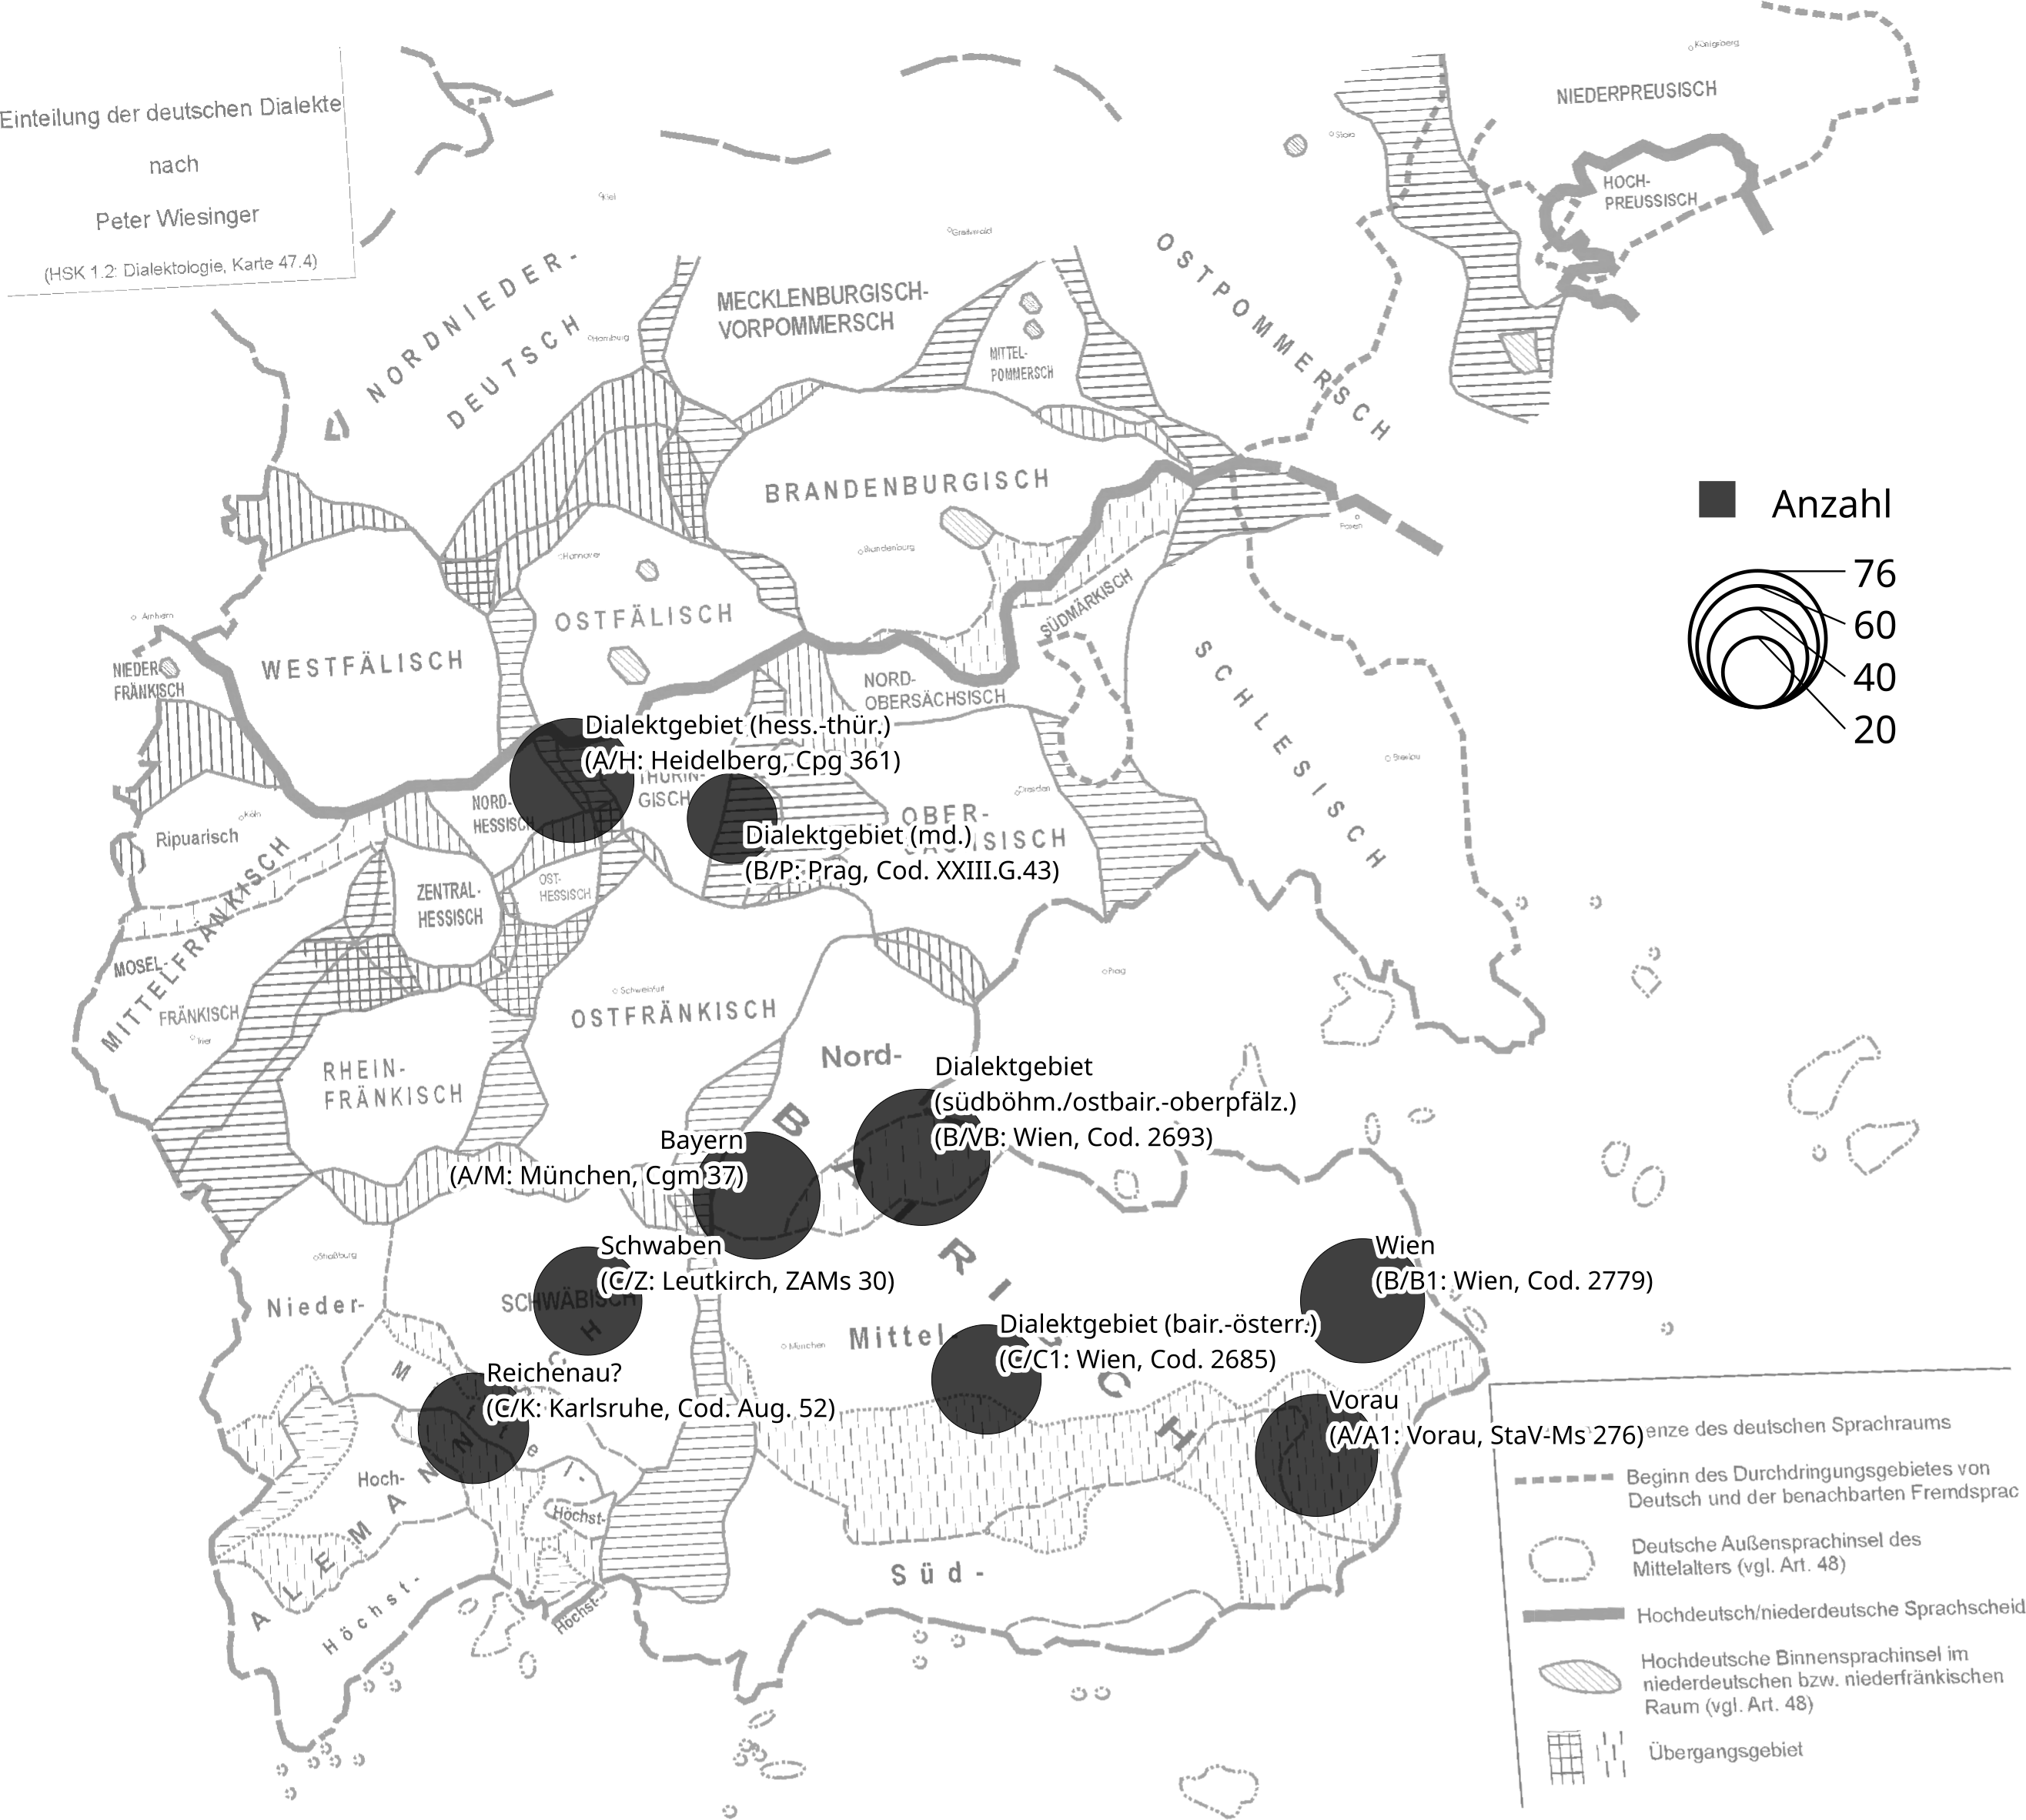
\includegraphics[
	width=\textwidth,
]{./assets/grafiken/2022-03-07_belege_gebiet.png}
\caption[Anzahl der Belege für mhd.\ \norm{bėide} pro Sprachlandschaft und
Handschrift]{Anzahl der Belege für mhd.\ \norm{bėide} pro Sprachlandschaft
und Handschrift\nocite{wiesinger1983:rede}}
\label{fig:kartebelegzahl}
\end{figure}

Im Regelfall ist bei mittelalterlichen Handschriften keine genaue Einordnung in
Zeit und Raum möglich, da diese -- im Unterschied zu Urkunden -- oft keine
derartigen Selbstauskünfte bieten
\autocites[1309--1310]{wegera2000}[117--121]{bein2011}. Insofern sind bei
\citet{kc:C1}, \citet{kc:H}, \citet{kc:M}, \citet{kc:P} und \citet{kc:VB} nur
weitläufige Regionen als (dialekt-)geografische Bezugsgröße angegeben.%
% %
% 	\footnote{Die Liste der Siglen, mit denen die verschiedenen Textzeugen
% 		bezeichnet werden, kann dem Literaturverzeichnis entnommen werden.}
% %
Die Platzierung der Handschriften auf der Karte folgt weitestgehend den Angaben
des \citetitle{hsc} \nosh\autocite{hsc} sowie den größtenteils deckungsgleichen
Angaben in \citet{kcdigital,wolf:kckat}. Aufgrund der fehlenden Möglichkeit
einer genauen Ortszuweisung in den meisten Fällen haben die markierten Punkte
also lediglich Näherungscharakter und beanspruchen keinesfalls eine geografisch
exakte Festlegung auf den jeweiligen Kartenpunkt.

Darüber hinaus merkt \citet{klein1988} zur Handschrift \citet{kc:H} an, diese
Handschrift möge \textquote{zwar in Hessen entstanden sein},%
%
	\footnote{Der Terminus \q*{Hessen} ist aufgrund der Geschichte des
	Bundeslandes ungenau. Dem Textzusammenhang nach wird wohl die
	Sprachlandschaft gemeint sein, die nicht deckungsgleich mit dem Territorium
	des modernen Bundeslandes ist \autocite[vgl.~z.\,B.][853]{wiesinger1983}.}
%
aber \blockcquote[118]{klein1988}{im thüringisch-hessischen Schreibdialekt
geschrieben und zeugt somit nicht für eine rheinische, sondern für eine
thüringisch-hessische \q*{Kaiserchronik}\nocite{schroeder1895}-Rezeption}.
\textcites{kcdigital}[23]{wolf:kckat} geben mit
\citet[237--238]{millerzimmermann2007} vorsichtig \q{Hessen (Mainz?)} als
Entstehungsort an.
% Unter dem Kriterium der Dialektgeografie müsste also nach
% \posscite{klein1988} Dafürhalten der Punkt weiter nordöstlich im
% hessisch-thüringischen Übergangsgebiet verankert sein.
\phantomsection%
\label{phsec:vbherkunft}%
Darüber hinaus beobachtet \citeauthor{schneider1987a} abweichend von den
Angaben im \citetitle{hsc} und \citet{kcdigital}, dass der Text der Handschrift
\citet{kc:VB} regelmäßig die eher für das Mitteldeutsche typische Kennform
\norm{quam} \wdef{kam} neben bairischem \norm{chom} enthält. Obwohl sie dem
Schreiber Bemühungen zur Vermeidung von Dialektismen attestiert, erwägt sie als
Entstehungsort den südböhmischen oder ostbairisch-oberpfälzischen Raum
\autocite[226]{schneider1987a}.

Neben der räumlichen Dimension spielt bei sprachhistorischen Untersuchungen
auch der zeitliche Bezug eine Rolle. Textzeugen der \citet{kc} finden sich vom
letzten Viertel des 12.~Jahrhunderts \autocites{kc:A1} bis ins späte
16.~Jahrhundert \autocite{kc:T}, wobei das Gros ins 13./14.~Jahrhundert fällt.
Die in der vorliegenden Untersuchung berücksichtigten Handschriften der
\citet{kc} entstanden zwischen dem letzten Viertel des 12.~Jahrhunderts und dem
Ende des 15.~Jahrhunderts, wie in \cref{fig:zeitstrahl} gezeigt. Die für die
Auswertung relevanten Textzeugen verteilen sich -- neben \citet{kc:A1} aus dem
12.~Jahrhundert -- auf die beiden Jahrhundertviertel um 1300 und stehen damit
zeitlich den Urkunden des \citetitle{cao} nahe.

\begin{figure}[p]
\centering
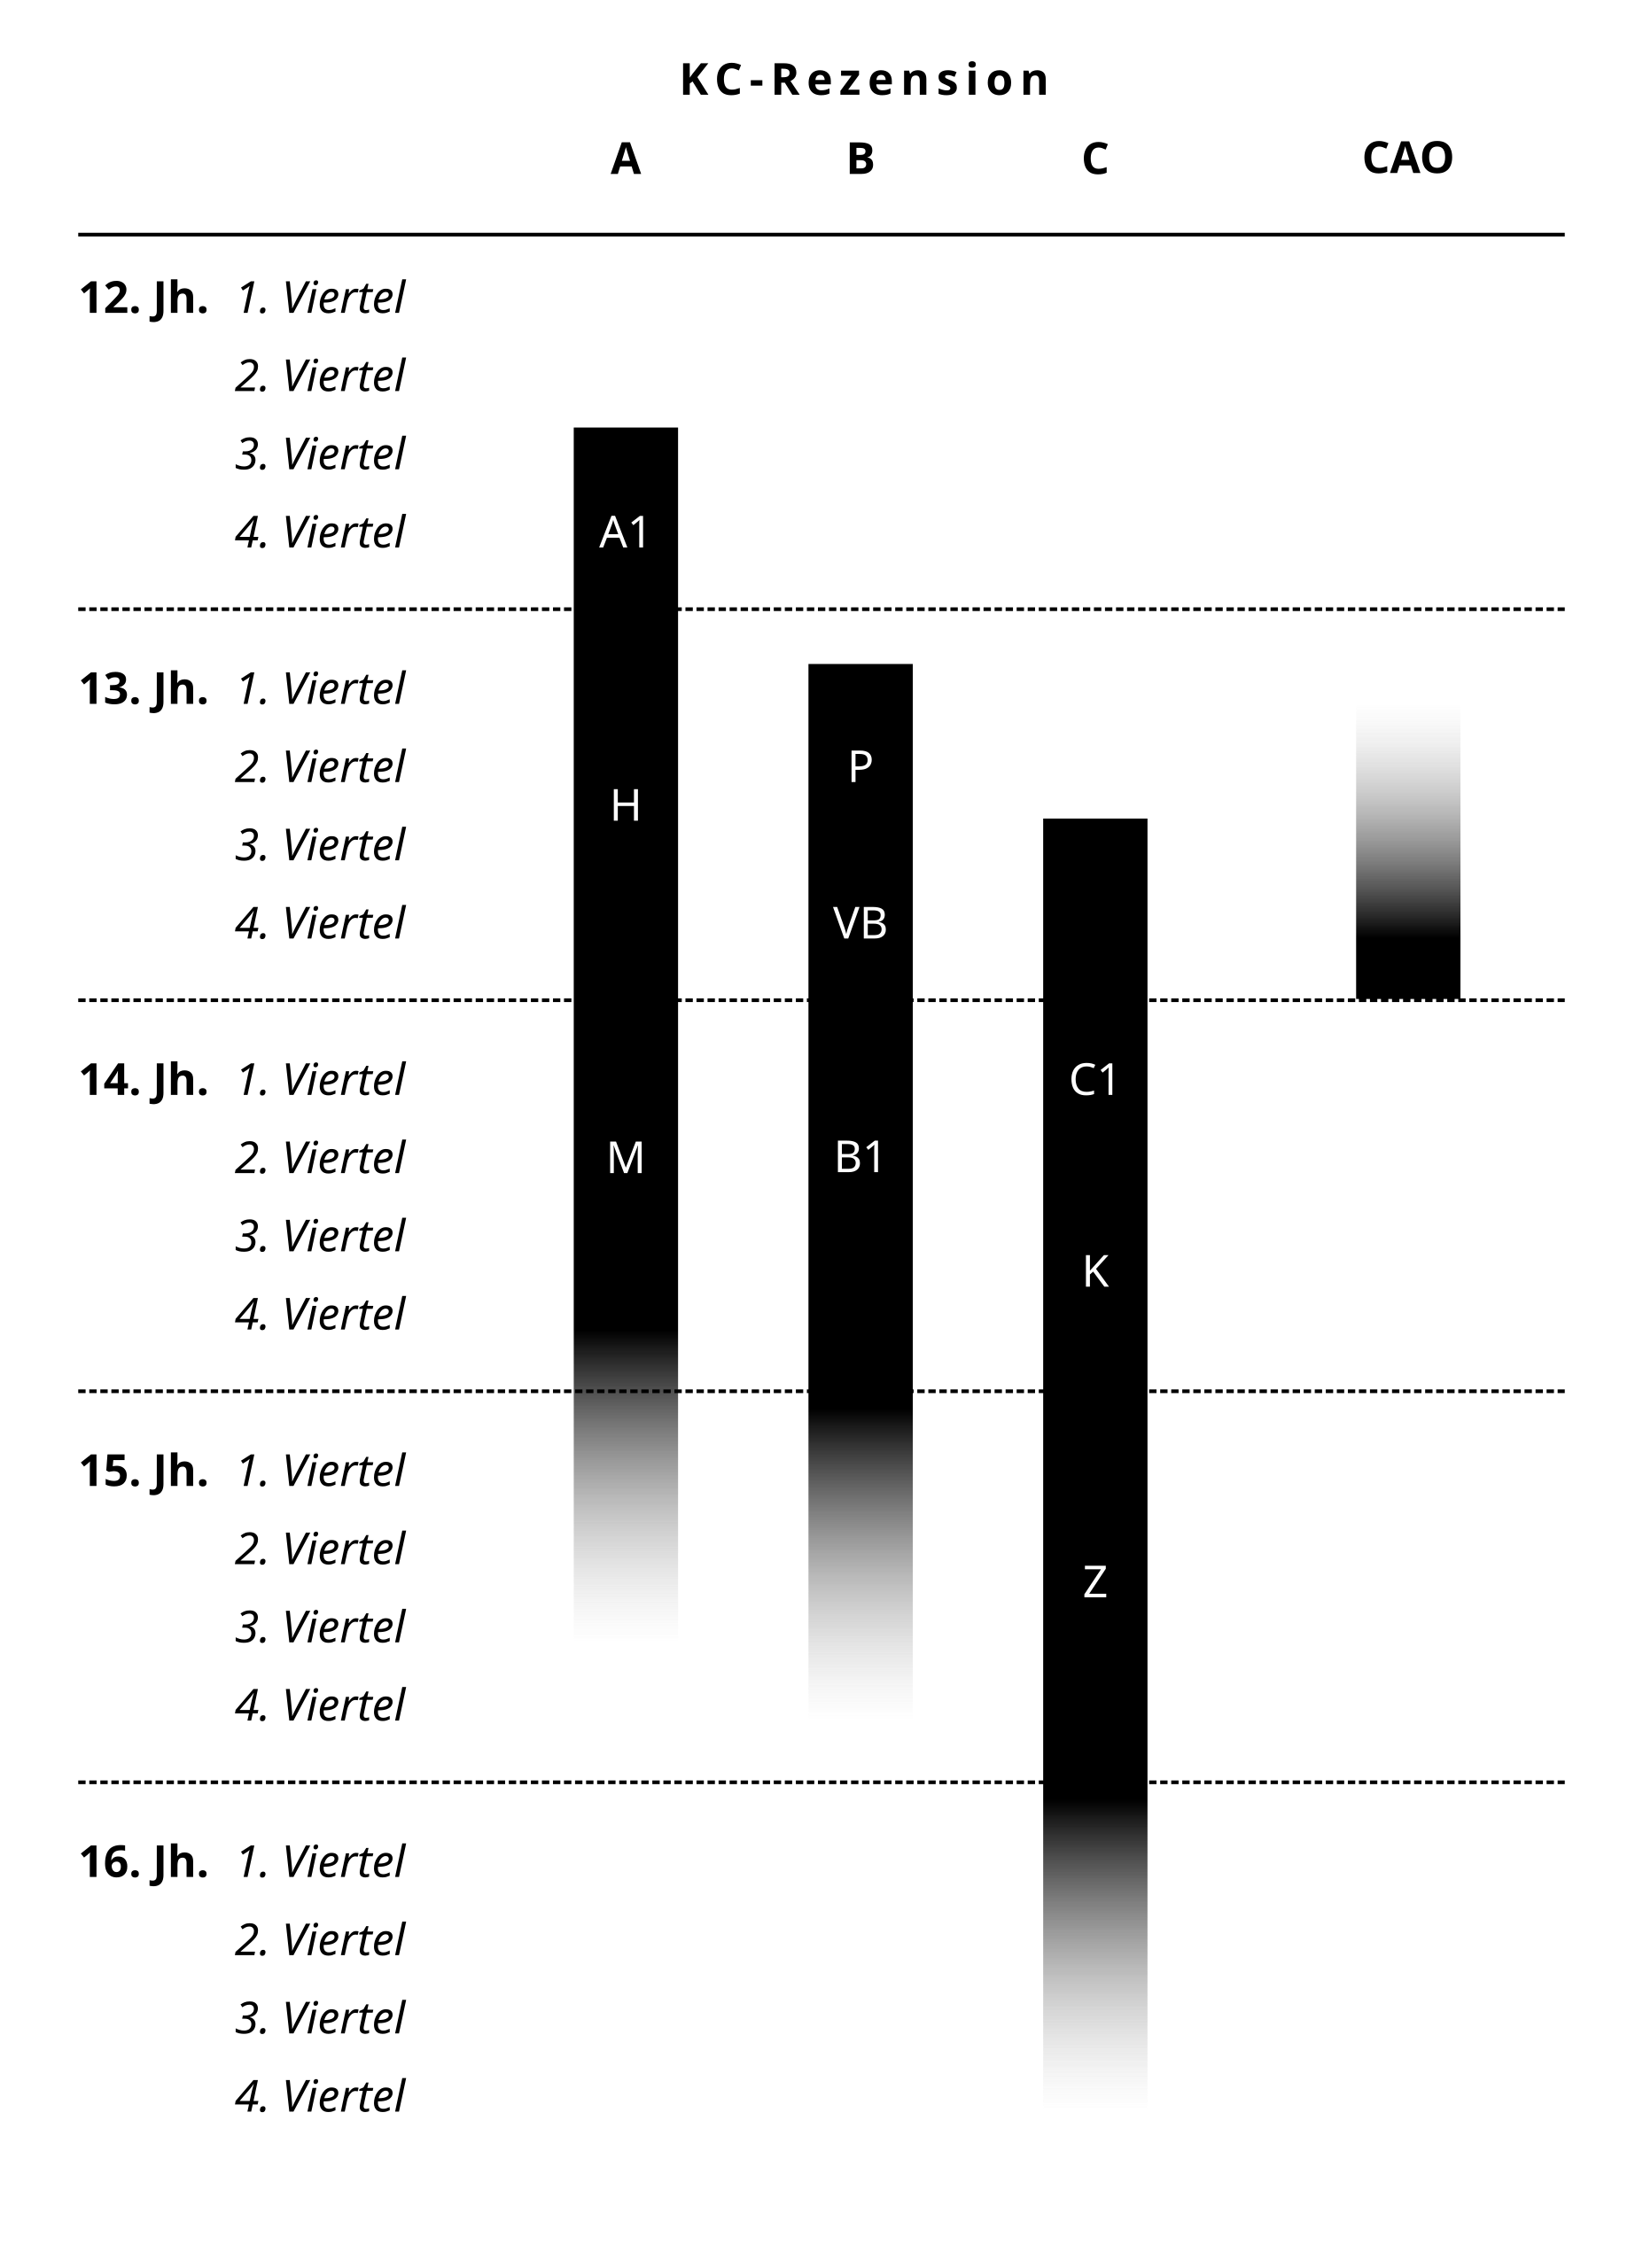
\includegraphics[
	height=.75\textheight,
]{./assets/grafiken/ueberlieferungszeitraeume.png}
\caption{Zeitliche Verteilung der untersuchten Handschriften und Urkunden}
\label{fig:zeitstrahl}
\end{figure}

\section{Targets nach Personenmerkmalen des Controllers}
\label{sec:kctargpers}

\subsection{Nominale Controller}

Wie bei der Belegsammlung zum \citetitle{cao} fällt die Belegmenge für den
direkten Bezug von \norm{bėide} auf zwei nominale Controller im ausgewerteten
\citet{kc}-Material gering aus. Für den hier untersuchten syntaktischen Kontext
liegen zwei Belege vor; zusammen mit der Kombination von Substantiv und
Pronomen sind es vier. Bei den zum Vergleich gesammelten Belegen zur direkten
Abhängigkeit von einzelnen Controllern im Plural finden sich dagegen 19
Beispiele.

\subsubsection{Kombinierte nominale Controller}
\label{subsubsec:conomctrlpers}

Das Beispiel und das Schema in \cref{ex:beid2subst} verdeutlichen den
syntaktischen Kontext, der im Folgenden zu untersuchen sein wird. Der Quantor
\norm{bėide} bezieht sich als Target direkt auf zwei Controller,
\lit{Willehalm} und \lit{Dietreich}, ohne dass eine Pronominalform dazwischen
steht.

\begin{exe}
\ex \label{ex:beid2subst}
	\begin{tikzpicture}[baseline=(1a_lb.base)]
	\node at (0,2)  (1a)    {\lit{Willehalm}};
	\node           (1a_box)[draw,rectangle,fit=(1a)] {};
	\node           (1a_lb) [above=.5ex of 1a_box, font=\mynodefont]
	                        {Controller 1};

	\node at (0,0)  (1b)    {\lit{Dietreich}};
	\node           (1b_box)[draw,rectangle,fit=(1b)] {};
	\node           (1b_lb) [above=.5ex of 1b_box, font=\mynodefont]
	                        {Controller 2};

	\node at (3,1) (2)      {\lit{baíde}};
	\draw (2) node (2_box)  [draw,rectangle,fit=(2)] {};
	\node (2_lb)   [above=.5ex of 2_box, font=\mynodefont] {Target};

	\draw [-latex] (1a_box) to [out=east, in=west] (2_box);
	\draw [-latex] (1b_box) to [out=east, in=west] (2_box);
	\end{tikzpicture}\\

\sn \gll \textbf{Willehalm} vnd \textbf{Dietreich}. \\
		Willehalm[\Nom.\Sg.\MascM] und Dietrich[\Nom.\Sg.\MascM] \\
\sn \gll wurden \textbf{baíde} da erſlagen. \\
		wurden beide-\Nom.\Pl.\MascM.\St{} da erschlagen \\
	\needspace{1\baselineskip}
	\begin{taggedline}{\parencite[\pno~83\vb, 36--37]{kc:C1}}
		\wdef{Willehalm und Dietrich wurden beide dort erschlagen.}
	\end{taggedline}
\end{exe}

Die erwähnten vier Belege, bei denen ein Target \norm{bėide} in einer
direkten Kongruenz\-beziehung zu zwei Substantiven steht, verteilen sich auf
nur drei verschiedene Parallelstellen, was die Menge an Kombinationen von
Personenmerkmalen äußerst reduziert. \cref{tab:koordnomctrl} gibt eine
Übersicht über die Zahl der Belege für den jeweiligen Flexionstyp und die
zugehörige Kombination der Personenmerkmale der Controller im hier besprochenen
syntaktischen Kontext.

\begin{table}
\centering
\caption{Flexion nach Personenmerkmalen der kombinierten nominalen Controller}
\begin{tabular}{
	l l
	r r
	r
}
\toprule
\textbf{Controller 1}
	& \textbf{Controller 2}
	& \textbf{bėide}
	& \textbf{bėidiu}
	& \textbf{Summe}
	\\

\midrule

\Tsg.\MascM & \Tsg.\MascM &  2 &  1  &  3 \\
\Tsg.\FemF  & \Ssg\subM   &    &  1  &  1 \\

\midrule

\mc{2}{l}{Summe}          &  2 &  2  &  4 \\

\bottomrule
\end{tabular}
\label{tab:koordnomctrl}
\end{table}

Von den drei Belegen zur Kombination zweier maskulin-männlicher Referenten sind
zwei derselben Parallelstelle zugehörig: Der Beleg in \cref{ex:dietwill_2}
wurde eingangs zitiert, er sei hier noch einmal im Kontext seiner
Parallelstelle in \cref{ex:dietwill_3} wiedergegeben. Wie erwartet zeigt der
Quantor für diese Merkmalskombination die Form \norm{bėide} in allen Fällen.
Zur dritten Stelle mit \norm{bėidiu} siehe \cref{ex:babstimbaideu}.

\begin{exe}
\ex \label{ex:dietwill} % 203
	\begin{xlist}
	% \ex \label{ex:dietwill_1}
	% 	\lit{\textbf{Dietrich} vnd \textbf{Willehalm} \\
	% 	Wurden zewurmtz \textbf{peid} erſlagen.}
	% 	\begin{taggedline}{\parencite[\pno~124\va, 3--4]{kc:M}}
	% 	\trans \wdef{Dietrich und Willehalm wurden in Worms beide erschlagen.}
	% 	\end{taggedline}

	\ex \label{ex:dietwill_2}
		\begin{taggedline}{\parencites[\pno~83\vb, 36--37]{kc:C1}}
		\gll \textbf{Willehalm} vnd \textbf{Dietreich}. \\
			Willehalm[\Nom.\Sg.\MascM] und Dietrich[\Nom.\Sg.\MascM] \\
	\sn \gll wurden \textbf{baíde} da erſlagen. \\
			wurden beide-\Nom.\Pl.\MascM.\St{} da erschlagen \\
		\end{taggedline}

	\ex \label{ex:dietwill_3}
		\gll \textbf{Wilhalm} vnd \textbf{dietrich} \\
			Willehalm[\Nom.\Sg.\MascM] und Dietrich[\Nom.\Sg.\MascM] \\
	\sn \gll Wurden \textbf{baide} do erſlagen \\
			wurden beide-\Nom.\Pl.\MascM.\St{} da erschlagen \\
		\begin{taggedline}{\parencites[\pno~95\vb, 12--13]{kc:K}}
		\trans \wdef{Willehalm und Dietrich wurden beide dort erschlagen.}
		\end{taggedline}

	% \ex \label{ex:dietwill_4}
	% 	\begin{taggedline}{\parencite[\pno~326\ra, 23--24]{kc:Z}}
	% 	\lit{\textbf{Wilhalm} vnd \textbf{dietreiche} \\
	% 		Wurden \textbf{baide} da erſlagen}
	% 	\end{taggedline}
	\end{xlist}
\end{exe}

Belege für die Kombination von maskulin-männlichen und feminin-weiblichen
Substantiven ($\MascM+\FemF$, $\FemF+\MascM$) liegen im hier untersuchten
Kontext zumindest formal keine vor. Es gibt allerdings einen Einzelbeleg für
die Kombination von weiblicher und männlicher Referenz bei Substantiv und
Personal\-pronomen, der in \cref{ex:mutterdu} wiedergegeben wird.

\begin{exe}
\ex\label{ex:mutterdu}
	\gll Zvͦ dem \textbf{chûnig} ſprach er ſan \textelp{} \\
		zu dem König[\Dat.\Sg.\MascM] sprach er sodann {} \\
\sn \gll Dein \textbf{m\sscr{u}{o}ter} vnd \textbf{dv} \\
		dein Mutter[\Nom.\Sg.\FemF] und \Ssg\subM.\Nom{} \\
\sn \gll Schv̂ln \textbf{beideu} chv̂men {dar zvͦ} \\
		sollen beide-\Nom.\Pl.\NeutMF.\St{} kommen dahin \\
	\begin{taggedline}{\parencite[\pno~23\rc, 5--14]{kc:B1}}
		\trans \wdef{Zum König sprach er sodann: \enquote{\textelp{} Deine
		Mutter und du sollt beide dahin kommen.}}
	\end{taggedline}
\end{exe}

Hier verbirgt sich hinter dem \lit{dv} \wdef{du} trotz fehlender
Genusmarkierung beim Pronomen der 2.\ Pers.\ Sg.\ ein männlicher Referent,
nämlich der \lit{chûnig} \wdef{König}, der direkt angesprochen wird. Der Beleg
passt damit in das Bild, das schon die Auswertung der Urkunden ergeben hat.
Auch bei Pro\-nomina ohne Genusmarkierung tritt aufgrund der referenzierten Personenmerkmale bei kombiniertem Bezug die
neutrale Form auf.

\phantomsection
\label{phsec:babstimbaideu}
Der Beleg in \cref{ex:babstimbaideu} mit \norm{bėidiu} in Bezug auf zwei
männliche Referenten wurde bereits erwähnt. Die Passage wurde hier so
interpretiert, dass sich \lit{ím} \wdef{ihm} auf \lit{Karle} \wdef{Karl (der
Große)} bezieht, also nicht auf \lit{wideme} \wdef{Dotierungen, Stiftungen}
\autocite[vgl. zur  Definition][\pno~\fw{wideme}]{lexer:mhdhwb} und
\lit{zehende} \wdef{Zehnten}. Letzteres Wortpaar steht im Genitiv Plural
\autocite[vgl.][341]{paul2007}, sodass die erwartete Kongruenzform des
Quantors regelmäßig \norm{bėider(e)} \wdef{beider} lauten müsste. Andere Belege
mit \norm{bėidiu} als Genitivform wurden weder für diese Handschrift noch für
die anderen exzerpiert.%
%
	\footnote{In Bezug auf den Text der Edition von
	\nosh\citet{schroeder1895} übersetzt \citet[249]{mayer1874}:
	\blockquote{Als König Karl dann zu Gericht saß, trat der Pabst vor ihn hin
	und klagte, daß die Rechte, welche seinen Vorfahren seien verliehen worden,
	ihm von den Römern entrissen wurden, so seien ihm namentlich Zehenten und
	Widdume genommen}; vgl. auch \citet[83]{weis2022}.}

\begin{exe}
\ex\label{ex:babstimbaideu}
	\gll \textbf{Karle} an daz gerichte ſaz \\
		Karl[\Nom.\Sg.\MascM] an das Gericht saß \\
\sn \gll Der \textbf{babſt} klegt \textbf{ím} daz \\
		der Papst[\Nom.\Sg.\MascM] klagte \Tsg.\MascM.\Dat{} dass \\
\sn \gll Der wideme vnd der zehende gar \\
		der Dotierungen und der Zehnten gar \\
\sn \gll Waͤren \textbf{baid\sscr{u}{ı}} worden bar \\
		wären beide-\Nom.\Pl.\NeutM.\St{} geworden ledig \\
\sn \gll Von ſínen vorvarn \\
		von seinen Vorfahren \\
	\begin{taggedline}{\parencites%
	% [85\vb, 22--25]
	[\pno~85\vb, 22--24]{kc:K}[vgl. abweichend][14383--14385]{schroeder1895}}
	\trans \wdef{Karl setzte sich zu Gericht. Der Papst klagte ihm, dass
		\textins{sie} beide an Dotierungen und gar an Zehnten ledig geworden
		wären durch seine Vorfahren.}
	\end{taggedline}
\end{exe}

Erfahrungsgemäß sollte man vorsichtig sein, Erwartungen an die Grammatik
mittelhochdeutscher Texte zu stellen. Jedoch ist die Form \lit{beider} in
\citet{kc:K} ansonsten die für den Gen.\ Pl.\ regelmäßig belegte, wie die
Beispiele in \cref{ex:k_beider} zeigen, sodass davon ausgegangen werden kann,
dass sich \lit{baidiu} an dieser Stelle tatsächlich auf Karl und den Papst
bezieht.

% K_008r-a.line_12,Sí hetten grôzze wu̍nne,54032
% K_008r-a.line_13,Zuͦ ír baider libe,54033

% K_009r-b.line_25,V̍nſer baider kínt,54258
% K_009r-b.line_26,Bevilch ich allen die hie ſínt,54259

% K_026r-a.line_02,Do mínnet oͮch du̍ vrowe ín,56973
% K_026r-a.line_03,Daz waz ír baider gewín,56974

% K_028v-b.line_36,In Rome bi ír baider zít,57461
% K_028v-b.line_37,Huͦb ſich vrlu̍g vnd ſtrit,57462

% K_067v-b.line_31,Jr baider ſtrit ſich gezoch,63837
% K_067v-b.line_32,Vf aín brugge vil hoch,63838

% K_076v-b.line_08,Do waz ir baider mítwiſt,65329
% K_076v-b.line_09,Gezogen ſich wiſſe criſt,65330
% K_076v-b.line_10,Aín Jar vnd acht wochan,65331

% K_103v-b.line_27,Daz waz ír baider vngewín,69959

\begin{exe}
\ex \label{ex:k_beider}
	\begin{xlist}
	\ex \label{ex:k_beider_1}
		\gll V̍nſer \textbf{baider} kínt \\
			unser beide-\Gen.\Pl.\St{} Kind \\
	\sn \gll Bevilch ich allen die hie ſínt \\
			befehle ich allen die hier sind \\
		\begin{taggedline}{\parencites%
			[\pno~9\rb, 25--26]{kc:K}[vgl.]%
			[\pno~8\vb, 27--28]{kc:C1}%
			% [\pno~6\va, 13--14]{kc:VC}%
			[\pno~31\va, 3--4]{kc:Z}%
			[abweichend][\pno~7\va, 3--4]{kc:A1}%
			[\pno~9\va, 42--43]{kc:H}%
			[\pno~15\va, 14--15]{kc:P}%
			[1639]{schroeder1895}
		}
		\trans \wdef{Unser beider Kind befehle ich allen an, die hier sind.}
		\end{taggedline}

	\ex \label{ex:k_beider_2}
		\gll In Rome bi ír \textbf{baider} zít \\
			in Rom bei ihr beide-\Gen.\Pl.\St{} Zeit \\
	\sn \gll Huͦb ſich vrlu̍g vnd ſtrit \\
			hob sich Krieg und Kampf \\
		\begin{taggedline}{\parencites
			[\pno~28\vb, 36--37]{kc:K}[vgl.]%
			% [\pno~17\va, 31--32]{kc:VC}%
			[\pno~93\va, 26--\pno~94\ra, 1]{kc:Z}[abweichend]%
			[\pno~14\va, 49--50]{kc:B1}%
			[\pno~24\ra, 30--31]{kc:VB}%
			[\pno~42\ra, 17--18]{kc:P}%
			[\pno~20\vb, 9--10]{kc:A1}%
			[\pno~36\rb, 6--7]{kc:M}%
			[\pno~28\rb, 39--40]{kc:H}%
			[4837--4838]{schroeder1895}%
		}
		\trans \wdef{Zu ihrer beider Zeit erhoben sich in Rom Kampf und Krieg.}
		\end{taggedline}

	\ex \label{ex:k_beider_3}
		\gll Daz waz ír \textbf{baider} vngewín \\
			Das war ihr beide-\Gen.\Pl.\St{} Verlust \\
		\begin{taggedline}{\parencites%
			[\pno~103\vb, 27]{kc:K}[vgl.]
			[\pno~91\va, 10]{kc:C1}%
			[\pno~60\va, 34]{kc:VC}%
			[\pno~352\ra, 6]{kc:Z}%
			[208]{schroeder1895}%
		}
		\trans \wdef{Das war ihr beider Verlust.}
		\end{taggedline}
	\end{xlist}
\end{exe}

% Bei den anderen Belegen in dem hier besprochenen Kontext handelt es sich um
% diejenigen in \cref{ex:romelat}
% \autocites[zu][11416--11417]{schroeder1895}[vgl. außerdem][69\ra,
% 29--30]{kc:H}, die in die \cref{tab:koordnomctrl} keinen Eingang gefunden
% haben, da \norm{bėide} in einer potentiellen Ausgleichsposition vor Vokal
% steht. In diesem Fall werden die Eigennamen \norm{Rôme} \wdef{Rom} und
% \norm{Lâterân} \wdef{Lateran} miteinander kombiniert. In beiden Fällen
% handelt es sich um Orte, also um Inanimata.

% \begin{exe}
% \ex \label{ex:romelat} % 211
% 	\begin{xlist}
% 	% \ex \begin{taggedline}{\parencite[\pno~49\vb, 14--16]{kc:A1}}
% 	% 	\lit{\textbf{rome}
% 	% 		unt \textbf{lateran}. \\ woͮrden im \textbf{baide} under%
% 	% 		tan.}
% 	% 	\end{taggedline}
% 	%	\label{ex:romelat_1}

% 	\ex \begin{taggedline}{\parencite[\pno~31\vb, 18--19]{kc:B1}}
% 		\lit{\textbf{Rom} vnd \textbf{lateran} \\
% 			wurden im \textbf{peid} vndertan}
% 		\end{taggedline}
% 		\label{ex:romelat_2}

% 	\ex \begin{taggedline}{\parencite[\pno~82\va, 45--46]{kc:VB}}
% 		\lit{\textbf{Rome} vnd \textbf{lateran} \\
% 			Wurden ím \textbf{bede} vndertan.}
% 		\end{taggedline}
% 		\label{ex:romelat_3}

% 	\ex \begin{taggedline}{\parencite[\pno~68\vb, 13--14]{kc:K}}
% 		\lit{\textbf{Rome} vnd \textbf{Lateran} \\
% 			Wurden ím \textbf{baidú} vndertan}
% 			\label{ex:romelat_4}
% 	\end{taggedline}

% 	% \ex \begin{taggedline}{\parencite[\pno~229\ra, 6--7]{kc:Z}}
% 	% 	\lit{\textbf{Rome} vnd \textbf{latran} \\
% 	% 		Wurden Im \textbf{baide} vndertan}
% 	% 	\end{taggedline}
% 	%	\label{ex:romelat_5}
% 		\trans \wdef{Rom und der Lateran wurden ihm beide untertan.}
% 	\end{xlist}
% \end{exe}

% \phantomsection
% \label{phsec:conomctrlpers}
% Es wurde angenommen, dass \norm{Rôme} gemäß \citet[484]{lexer2} auch hier
% neutrales Genus aufweist. Das Genus von \norm{Lâterân} dagegen konnte nicht
% einfach erörtert werden. An allen Stellen zu \norm{Lâterân}, die
% \citet[422]{schroeder1895} ausweist \autocite[4154, 5953, 6008, 6820, 11416,
% 11591, 11748, 12700, 14630]{schroeder1895}, steht der Name des Ortes ohne
% Artikel, gemeinhin in einer Doppelformel zusammen mit \norm{Rôme}. Eine Suche
% in der Mittelhochdeutschen Begriffsdatenbank\nocite{mhdbdb} förderte nur
% einen einzigen Beleg mit Artikel zutage \cref{ex:latoranfem}.
% %
% \begin{exe}
% \ex\label{ex:latoranfem}
% 	\gll Der buwte die grossen Latoran \\
% 	     der baute \Def.\Acc.\Sg.\FemI{} groß-\Acc.\Sg.\FemI.\Wk{} Lateran \\
% 	\begin{taggedline}{\parencite[25086]{koppitz1926}}
% 	\trans \wdef{Der [=~Nero] baute den großen Lateran.}
% 	\end{taggedline}
% \end{exe}

% Anders als im modernen Sprachgebrauch handelt es sich hier bei \lit{Latoran}
% \wdef{Lateran} um ein Femininum \autocite[\FemI;][182]{ksw2}. Diesen einen
% Beleg zu generalisieren erschien nicht ratsam, daher wurde hier letztendlich
% die Annotation \UnknI\ (unbekanntes Genus, unbelebt) für \norm{Lâterân}
% gewählt. Ob gleiches oder verschiedenes Genus vorliegt, kann also nicht
% erörtert werden. In den Urkunden des \citetitle{cao} geht die Kombination
% zweier unbelebter Substantive allerdings generell mit großer Affinität zur
% Form \norm{bėidiu} einher, unabhängig von deren Genus. Trotz der Unbelebtheit
% beider Referenten in \cref{ex:romelat} weisen die beiden bairischen
% Handschriften \citet{kc:B1} und \citet{kc:VB} eine \norm{e}-Form auf
% \crefrange{ex:romelat_2}{ex:romelat_3}, die alemannische Handschrift
% \citet{kc:K} zeigt dagegen die \norm{iu}-Form \cref{ex:romelat_4}. Auffällig
% ist, dass \norm{bėide} an dieser Stelle in einer Hiatusposition steht, denn
% das nächste Wort \norm{undertân} \wdef{untertan} fängt mit einem Vokal an.

% \citet{askedal1973} merkt bezüglich eines ähnlichen Falls in seiner
% Auswertung der \citetitle{maroldschroeder1969}-Edition von
% \citet{maroldschroeder1969} an, dass denkbar sei, dass die Flexionsendung
% \norm{iu} in Hiatuspositionen grafisch zu \orth{e} neutralisiert und bei der
% Rezitation apokopiert werde \autocite[90--91]{askedal1973}. Apokope ist auch
% im Kontext von \cref{ex:romelat} plausibel, wie am folgenden Skansionsschema
% deutlich wird:
% %
% \begin{center}
% \begin{tabular}[t]{@{}
% c @{}  c @{~} c @{~}
% c @{~} c @{~} c @{~}
% c @{}  c @{~} c @{~}
% c @{}  c @{~} c @{~}
% }
%   \itshape wur & \itshape den   & 
% & \itshape im  & \itshape beidẹ & 
% & \itshape un  & \itshape der   & - 
% & \itshape tân & \itshape       & \\

%   \char"F70B   & \char"F70A     & |
% & \char"F70B   & \char"F70A     & |
% & \char"F70B   & \char"F70A     & |
% & \char"F705   &                & ||
% \\
% \end{tabular}
% \end{center}
% %
% % Ohne Ausfall des Endvokals in \norm{bėide} müsste \norm{-den im}
% entweder % zwei kurze Silben (⏑⏑) bilden, oder es käme zum Hebungsprall
% zwischen % \norm{im bei-} (\char"F70B \char"F70C). Beide Varianten machen den
% Vers % holprig; mit Apokope beim Quantor wird er dagegen metrisch regelmäßig.

% Die Apokope wurde in \cref{ex:romelat_2} grafisch ausgeführt, wobei es sich
% dort auch um die im Bairischen generell seit dem 13.~Jahrhundert verbreitete
% Schwa-Apokope handeln kann \autocites{lindgren1953}[109--111]{paul2007}. Ob in
% den unterschiedlichen \citet{kc}-Handschriften phonologische Faktoren
% gemäß \citet{askedal1973} tatsächlich \emph{regelmäßig} einen Einfluss auf
% die Wahl der adjektivischen Flexionsendung haben, ist gesondert zu
% untersuchen.

\subsubsection{Einfache nominale Plural-Controller}
\label{subsubsec:nomctrlpers}

In diesem Abschnitt werden zum Vergleich Belege wie der in
\cref{ex:beidplsubst} diskutiert. Das Target \lit{bêde} \wdef{beide} ist hier
ebenfalls unmittelbar auf seinen Controller bezogen. Im Vergleich zum vorigen
Abschnitt handelt es sich beim Controller jedoch nicht um die Kombination von
Substantiven, sondern nur um ein einzelnes Substantiv, das im Plural steht.

\begin{exe}
\ex \label{ex:beidplsubst}
	\begin{tikzpicture}[baseline=(1_lb.base)]
	\node (1)      [align=center]
	               {\lit{gotes boten}};
	\node (1_box)  [draw,rectangle,fit=(1)] {};
	\node (1_lb)   [above=.5ex of 1_box, font=\mynodefont]{Controller};

	\node (2)      [right=4em of 1_box, align=center]
	               {\lit{bêde}};
	\draw (2) node (2_box1) [draw,rectangle,fit=(2)] {};
	\node (2_lb1)  [above=.5ex of 2_box1, font=\mynodefont] {Target};

	\draw [-latex] (1_box) to (2_box1);
	\end{tikzpicture}\\

\sn \gll die \textbf{gotes boten} \textbf{bêde} \\
		 die Gottesboten[\Nom.\Pl{}.\MascM] beide-\Nom.\Pl.\MascM.\St{} \\
	\begin{taggedline}{\parencite[7845]{schroeder1895}}
	\trans \wdef{die beiden Gottesboten}
	\end{taggedline}
\end{exe}

Kontexte, in denen \norm{bėide} in einer direkten Kongruenzbeziehung mit einem
einzigen Substantiv im Plural steht, sind auch in der \citet{kc} im Vergleich
zu Kontexten mit kombinierter Referenz zahlreicher vorhanden.
\cref{tab:simpnomctrla} zeigt ihre Verteilung nach Personenmerkmalen und
Flexionstyp.

%	\begin{xlist}
%	\ex Vorangestellt: \\
%		\lit{Die \textbf{baide} \textbf{gottes botten}}
%		\begin{taggedline}{\parencites[\pno~155\ra, 24]{kc:Z}[vgl.][7845]{schroeder1895}}
%		\trans \wdef{die beiden Gottesboten}
%		\end{taggedline}
%		\label{ex:beidplsubst_1}

%	\ex Nachgestellt: \\
%		\lit{di \textbf{gotes boten} \textbf{bede}}
%		\begin{taggedline}{\parencites[\pno~33\vb, 24]{kc:A1}[vgl.][7845]{schroeder1895}}
%		\trans \wdef{die beiden Gottesboten}
%		\end{taggedline}
%		\label{ex:beidplsubst_2}

%	\ex Gefloatet (Distanzstellung): \\
%		\lit{Die lieben \textbf{her geſellen}. \\
%			Wonten da vber naht \textbf{beide}.}
%		\begin{taggedline}{\parencites[\pno~100\va, 24--25]{kc:VB}[vgl.][15038--15039]{schroeder1895}}
%		\trans \wdef{Die lieben Kampfgefährten wohnten da beide über Nacht.}
%		\end{taggedline}
%		\label{ex:beidplsubst_3}
%	\end{xlist}

\begin{table}
\centering
\caption{Flexion nach Personenmerkmalen der einfachen nominalen Controller}
\begin{tabular}{l r r r}
\toprule
\textbf{Controller}
	& \textbf{bėid(e)}
	& \textbf{bėidiu}
	& \textbf{Summe}
	\\

\midrule

\MascM  & 11 &  2 & 13 \\
\NeutM  &    &  1 &  1 \\
\NeutA  &    &  1 &  1 \\

\midrule

\FemI   &  1 &    &  1 \\

\midrule

Summe   & 12 &  4 & 16 \\

\bottomrule
\end{tabular}
\label{tab:simpnomctrla}
\end{table}

Mit elf Belegen zu fünf Stellen verteilen sich die meisten
\norm{bėid(e)}-Formen mit maskulin-männlichem Bezug wie nach formalen Kriterien
erwartet \autocite[vgl.][182]{ksw2}. Interessant sind in diesem Kontext die
Abweichungen, das heißt, die zwei Belege für \norm{bėidiu} mit
maskulin-männlichem Bezug. Diese werden in \cref{ex:richtherriu} wiedergegeben.
% Gemeinsam ist beiden Stellen, dass der Quantor gefloatet im Mittelfeld steht
% (vgl. \cpageref{phsec:richtherriu2}).
Starke Adjektive zeigen in \citet{kc:B1} ansonsten \norm{-iu} im Plural
regel\-mäßig nur bei den Neutra; Maskulina und Feminina sind dagegen stets
endungslos (vgl.~\cref{tab:kcadjdeclovw}).

\begin{exe}
\ex \label{ex:richtherriu}
	\begin{xlist}
	\ex \gll Die \textbf{rihtær} ſprachen \textbf{beideu} {dar zuͦ} \\
			die Richter[\Nom.\Pl.\MascM] sprachen beide-\Nom.\Pl.\NeutM.\St{}
			dazu \\
		\begin{taggedline}{\parencites[\pno~28\ra, 8]{kc:B1}[vgl.~abweichend][10090]{schroeder1895}} % 1140 mit Parallelstelle in H
		\trans \wdef{Die Richter äußerten sich beide dazu}
		\end{taggedline}
		\label{ex:richtherriu_1}

	\ex \gll Die \textbf{herren} baten ir ſa \\
			Die Herren[\Nom.\Pl.\MascM] baten ihr alsbald \\
	\sn \gll \textbf{Beideu} beſvnder \\
			beide-\Nom.\Pl.\NeutM.\St{} einzeln \\
		\begin{taggedline}{\parencites[\pno~31\va, 48--49]{kc:B1}[vgl.][11385--11386]{schroeder1895}} % 1112x
		\trans \wdef{Die Herren hielten alsbald jeweils beide um ihre Hand an.}
		\end{taggedline}
		\label{ex:richtherriu_2}
	\end{xlist}
\end{exe}

% Bei den Beispielen für $\NeutM$ in \crefrange{ex:chintpeide}{ex:baideuwarn}
% ist jeweils ein Beleg für beide der zwei Flexionstypen des Quantors
% vorhanden. Hier lohnt sich unbedingt der Vergleich mit einer größeren Menge
% Adjektive im gleichen syntaktischen Kontext.

% \begin{exe}
% \ex \label{ex:chintpeide}
% 	\lit{Do chavft ſie dív \textbf{chint} \textbf{peide}}
% 	\begin{taggedline}{\parencites[\pno~8\ra, 9]{kc:VB}[vgl. stark abweichend][1450]{schroeder1895}} % 1158x
% 	\trans \wdef{Da kaufte sie die Kinder beide}
% 	\end{taggedline}
% 	% → -e belegt für ACC.PL.N.ST, -iu überwiegt leicht
% \end{exe}

% In \cref{ex:chintpeide} bezieht sich \lit{chint} \wdef{Kinder} auf die beiden
% Brüder \lit{Nyceta} und \lit{Aquila} \autocites[7\vb,
% 30--31]{kc:VB}[vgl.][1428--1429]{schroeder1895}, insofern ist der männliche
% semantische Bezug hier gesichert. In der Stichprobe zu \citet{kc:VB} sind für
% attributive Adjektive des \Acc.\Pl.\N.\St\ in attributiven Kontexten sowohl
% \norm{iu}-Formen als auch einige \norm{e}-Formen vorhanden, ohne dass ein
% Unterschied nach Belebheit beobachtet werden kann: Alle acht Belege in der
% Stichprobe für diesen Annotationstyp sind unbelebt. Auch für \Acc.\Pl.\M.\St\
% ist zumindest ein (belebter) Beleg für \lit{-Ø} vorhanden. In jeder Hinsicht
% ist also davon auszugehen, dass sich \cref{ex:chintpeide} im grammatischen
% System der Handschrift \citet{kc:VB} normal verhält.

% Der Grund, weshalb sowohl \norm{iu} als auch \norm{e} in derselben Position
% des Paradigmas zu finden ist, lässt sich zum einen in der
% Nebensilbenabschwächung suchen, die im Lauf des späten Mittelalters
% schlussendlich auch \norm{-iu} erfasst und zu \norm{-e} werden lässt. Nach
% \citet{ksw2} breitet sich \norm{-e} ab der zweiten Hälfte des 13.
% beziehungsweise der ersten Hälfte des 14. Jahrhunderts vom Ostfränkischen und
% \textquote{minder stark} vom Alemannischen ins Bairische aus
% \autocite[266]{ksw2}. \citet{paul2007} zufolge wird \norm{-iu} bis zum
% Ende des 15.~Jahrhunderts dann vollständig durch \norm{-e} verdrängt
% \autocites[203]{paul2007}[vgl.][191--192]{reichmannwegera1993}.

\phantomsection
\label{phsec:baideuwarn}
Der Beleg zu \norm{bėidiu} bei einem Neutrum mit männlichem Bezug in
\cref{ex:baideuwarn}, ein Parallelbeleg zu dem in \cref{ex:babstimbaideu}
zitierten, enthält formale Kongruenz. Das Lexem \lit{warn} \wdef{Kinder} zu
mhd.\ \norm{barn} \wdef{Kind, Sohn; Jüngling, Held (?)}
\autocites[\pno~\fw{barn}]{mwb1}[vgl.~auch][53]{kroonen2013} bezieht sich hier
metaphorisch auf Karl den Großen und Papst Leo~III., die vom Kaiserchronisten
als Brüder dargestellt werden
\autocites[14370]{schroeder1895}[vgl.][83]{weis2022}. Obwohl sich \lit{warn}
also auf zwei erwachsene Männer bezieht, was die Wahrscheinlichkeit für
semantische Kongruenz erhöht (siehe \cref{sec:gendsex}), zeigt der Quantor in
formaler Übereinstimmung mit seinem Controller die neutrale Form.

\begin{exe}
\ex \label{ex:baideuwarn}
	\gll der wídem vnd der zehent gar. \\
		der Dotierungen und der Zehnten gar \\
\sn \gll wærn \textbf{baidev} \textbf{warn} bar. \\ % 1123
		wären beide-\Nom.\Pl.\NeutM.\St{} Kinder[\Nom.\Pl.\NeutM] ledig \\
	\begin{taggedline}{\parencites[\pno~75\rb, 3--4]{kc:C1}[vgl. abweichend][\pno~85\vb, 24]{kc:K}[][14384--14385]{schroeder1895}}
	\trans \wdef{an Dotierungen und Zehnten wären beide Kinder ledig}
	\end{taggedline}
\end{exe}

% Der Vollständigkeit halber sei angemerkt, dass auch in der Parallelstelle zu
% \cref{ex:baideuwarn} in \citet{kc:K} \cref{ex:baideuwarn2} die an sich
% neutrale Form \lit{baidu̍} mit direktem Bezug auf \lit{babſt} \wdef{Papst}
% und \lit{ím} \wdef{ihm} (=~\lit{Karle} \wdef{Karl der Große}) als
% morphologisch und semantisch eindeutige Maskulina auftritt. Der Quantor wird
% hier am ehsten als Pronominalisierung zu interpretieren sein. Formal steht
% \lit{baidu̍} nicht gefloatet im gleichen Teilsatz, sondern bildet das Subjekt
% eines neuen Satzes (vgl. \cpageref{phsec:baideuwarn3}).

% \begin{exe}
% \ex\label{ex:baideuwarn2} % 301
% 	\lit{\textbf{Karle} an daz gerichte ſaz \\
% 		Der \textbf{babſt} klegt \textbf{ím} daz \\
% 		Der wideme vnd der zehende gar \\
% 		Waͤren \textbf{baid\sscr{u}{ı}} worden bar}
% 	\begin{taggedline}{\parencites[\pno~85\vb, 22--24]{kc:K}[vgl. abweichend][14382--14385]{schroeder1895}}
% 	\trans \wdef{Karl setzte sich zu Gericht. Der Papst klagte ihm, dass beide an
% 		Dotierungen und gar an Zehnten ledig geworden wären \textelp{}}
% 	\end{taggedline}
% \end{exe}

Auch der Quantor in \cref{ex:beideuher} dekliniert nach dem neutralen Genus
gemäß formaler Kongruenz innerhalb der Nominalphrase (NP). In
\cref{tab:simpnomctrla} wurde dieser Beleg mit \SA\ gekennzeichnet, da
\lit{her} \wdef{Heer} bei der Annotation als Committee Noun
\autocite[211--213]{corbett2006} aufgefasst wurde: Der Begriff, obwohl formal
im Singular, bezieht sich in seiner Semantik auf eine Gruppe von Menschen. In
jedem Fall zeigt sich nicht das Fehlen von overter Flexion, die ansonsten in
der Stichprobe zu \citet{kc:B1} für den starken Nom./Akk.~Pl.~M./F. belegt ist.

\begin{exe}
\ex \label{ex:beideuher}
	\gll Der wær herre ûber \textbf{beideu} \textbf{her} \\
		der wäre Herr über beide-\Acc.\Pl.\NeutA.\St{} Heer[\Acc.\Pl.\NeutA] \\
	\begin{taggedline}{\parencites[\pno~31\rc, 3]{kc:B1}[zu][11272\psqq]{schroeder1895}} % 1110
	\trans \wdef{Der wäre Herr über beide Heere}
	\end{taggedline}
	% → der ist normal!
\end{exe}

Der Beleg für ein unbelebtes Femininum hat die Form \lit{baide}, insofern auch
hier der Quantor innerhalb der NP formale Kongruenz zeigt
\cref{ex:uozehende_2}, obwohl es sich um Körperteile handelt und damit um
etwas, von dem auszugehen ist, dass es eine mittlere Position zwischen den
Polen belebt und unbelebt einnimmt (vgl.~\cref{sec:gendsex} zur Annotation von
Genus bei Inanimata).

\begin{exe}
% \ex \label{ex:uozehende}
% 	\begin{xlist}
% 	\ex \lit{und die nag%-
% 			el die man durch ſine \textbf{baide} \textbf{u\sscr{o}{v}ze} ſlu%-
% 			ch.}
% 		\begin{taggedline}{\parencites[\pno~45\va, 11]{kc:A1}[10390]{schroeder1895}}
% 		\trans \wdef{und die Nägel, die man durch seine beiden Füße schlug}
% 		\end{taggedline}
% 		\label{ex:uozehende_1}

	\ex \gll Si wand ír \textbf{baide} \textbf{hênde} \\
			sie wand ihr beide-\Acc.\Pl.\FemI.\St{} Hand-\Acc.\Pl.\FemI{} \\
		\begin{taggedline}{\parencites[\pno~6\rb, 19]{kc:K}[vgl.][913]{schroeder1895}}
		\trans \wdef{Sie wand ihre beiden Hände.}
		\end{taggedline}
		\label{ex:uozehende_2}
% 	\end{xlist}
\end{exe}

% In \cref{ex:uozehende_1} ist aus syntaktischer Perspektive interessant, dass
% trotz overter Markierung von Personenmerkmalen beim Possessivpronomen
% \lit{ſine} \wdef{seine} (\Acc.\Pl.\F.\St) der nachfolgende Quantor ebenfalls stark
% dekliniert ist statt nach der Formregel die schwache Form *\lit{baiden}
% anzunehmen \autocite[vgl.][217--218]{ksw2}; \cref{ex:uozehende_2} ist dagegen
% vollkommen unauffällig.

\subsubsection{Zusammenfassung}

Die Belegstellen zum kombinierten direkten Bezug von \mbox{\norm{bėide}} auf
zwei Substantive fallen nicht aus dem Rahmen bisheriger Ergebnisse, wenn es
auch die geringe Belegzahl unmöglich macht, generelle Aussagen zu treffen. In
beiden Fällen zeigte sich die Form \norm{bėide} mit Bezug auf maskuline und
feminine Referenten. Im Fall der Kongruenz eines Quantors mit einem einzelnen
Substantiv im Plural wiesen die Targets innerhalb der NP ebenfalls formale
Kongruenz auf, doch liegen zwei Belege für neutrales \norm{bėidiu} bei
eindeutig maskulin-männlichem Bezug vor.

% Weitere vermeintliche Ausnahmen konnten durch die Rekonstruktion des
% adjektivischen Deklinationsparadigmas für die jeweiligen Handschriften
% aufgeklärt werden, auch unter Berücksichtigung des dialektgeografischen
% Zusammenhangs. Im Fall von \norm{bėide} als gefloatetem Quantor mit
% unbelebtem kombinierten Bezug konnte durch Überlegungen zur Versstruktur
% erklärt werden, warum entgegen der Erwartung die Form \norm{bėidiu} auftritt.

\subsection{Anaphorische Controller}

Mit 19 Stellen liegt der größere Teil des Belegmaterials zur \citet{kc} für die
Kongruenzrelation zwischen \norm{bėide} in indirekter Abhängigkeit von zwei
nominalen Controllern vor. Die Kombination von Substantiv und einem Pronomen
der ersten oder zweiten Person als Diskurs\-anker wird hier mitgezählt.
Textstellen mit indirektem Bezug zwischen Quantor und einzelnem Substantiv im
Plural sind neun vorhanden.

\subsubsection{Indirekter Bezug auf kombinierte nominale Controller}
\label{subsubssec:iconomctrlpers}

Hier soll zunächst der Kongruenzbezug zwischen kombinierten Controllern und
Quantor mit einem Pronomen als Verbindungsglied anhand der gesammelten Belege
untersucht werden.
% Die Kongruenzrelation zwischen Erstcontrollern und
% \wdef{beide}-Target ist in diesem Kontext also mittel\-bar.
Das Verhältnis zwischen Kongruenzcontrollern und Target wird in
\cref{ex:beidanactrl} illustriert.%
%
	\footnote{Auch für die \citet{kc} gilt, dass das Personalpronomen der
		3.~Pers.\ Pl.\ Nom./Akk. in der Regel zu \norm{si} ausgeglichen
		erscheint, also keine Differenzierung zwischen maskulin-femininem
		\norm{sie} und neutralem \norm{siu} nachzuvollziehen ist, vergleiche
		\textcites[213--214]{paul2007}[369, 390--397]{ksw2} sowie die
		Teiluntersuchung zur Form des Pronomens in
		\cref{subsubsec:monoflexionkc}.}

\begin{exe}
\ex\label{ex:beidanactrl}
	\begin{tikzpicture}[baseline=(1a_lb.base)]
	\node at (0,2)  (1a)    [gray]
	                        {\lit{muoter}};
	\node           (1a_box)[draw,gray,rectangle,fit=(1a)] {};
	\node           (1a_lb) [above=.5ex of 1a_box, gray, font=\mynodefont]
	                        {Controller 1};

	\node at (0,0)  (1b)    [gray]
	                        {\lit{sun}};
	\node           (1b_box)[draw,gray,rectangle,fit=(1b)] {};
	\node           (1b_lb) [above=.5ex of 1b_box, gray, font=\mynodefont]
	                        {Controller 2};    

	\node at (3,1) (2)      {\lit{si}};
	\draw (2) node (2_box1) [
	                    draw,
	                    gray,
	                    minimum height=3em,
	                    minimum width=3em,
	                    xshift=-.5ex,
	                    yshift=+.5ex,
	                    rectangle
	                ] {};
	\draw (2) node (2_box2) [
	                    draw,
	                    minimum height=3em,
	                    minimum width=3em,
	                    xshift=+.5ex,
	                    yshift=-.5ex,
	                    rectangle
	                ] {};
	\node           (2_lb1) [above=.5ex of 2_box1, gray, font=\mynodefont]
	                        {Target};
	\node           (2_lb2) [below=.5ex of 2_box2, font=\mynodefont]
	                        {Controller};

	\node at (6,1)  (3)      {\lit{baide}};
	\node           (3_box)  [draw,rectangle,fit=(3)] {};
	\node           (3_lb)   [above=.5ex of 3_box, font=\mynodefont]
	                        {Target};

	\draw [-latex,gray] (1a_box) to [out=east, in=west] (2_box1);
	\draw [-latex,gray] (1b_box) to [out=east, in=west] (2_box1);
	\draw [latex-]      (3_box)  to [yshift=1.5ex]      (2_box2);
	\end{tikzpicture}\\

\sn \gll Si nâmen di \textbf{muoter} mit dem \textbf{sun}, \\
		sie nahmen die Mutter[\Acc.\Sg.\FemF] mit dem Sohn[\Dat.\Sg.\MascM] \\
\sn \gll si viengen \textbf{si} bî dem hâre, \\
		sie fingen \Tpl\subMF.\Acc{} an dem Haare \\
\sn \gll si vuorten \textbf{si} \textbf{baide} zewâre \\
		sie führten \Tpl\subMF.\Acc{} beide-\Acc.\Pl.\M+\F\subMF.\St{}
			wirklich \\
\sn \gll vur die burch an daz velt \\
		vor die Stadt an das Ebene \\
	\begin{taggedline}{\parencite[14269--14272]{schroeder1895}}
	\trans \wdef{Sie nahmen die Mutter mit dem Sohn. Sie fingen sie an den
		Haaren. Ja, sie führten sie beide vor die Stadt zu der Ebene.}
	\end{taggedline}
\end{exe}

Auch wenn es sich bei \lit{muoter mit dem sun} \wdef{Mutter mit dem Sohn} nicht
strikt um eine syntaktische Koordination vom Typ \q*{\textsc{a} \fw{und}
\textsc{b}} handelt (vgl.~\cref{sec:erwkonjbegr} zur \q*{erweiterten}
Koordination), werden \lit{muoter} \wdef{Mutter} und \lit{sun} \wdef{Sohn}
durch \lit{si} \wdef{sie} kombiniert zusammengefasst. Der Quantor \lit{baide}
modifiziert dieses \lit{si} und kongruiert mit ihm. Der Quantor kongruiert
damit direkt mit dem Personalpronomen \lit{si} und indirekt mit \lit{muoter}
und \lit{sun}.

\Cref{tab:kcsimprefctrl} gibt die Belegverteilung in der \citet{kc} für die in
\cref{ex:beidanactrl} exemplarisch ausgeführte Kongruenzrelation wieder,
wobei auch hier nur Handschriften berück\-sichtigt wurden, die beide
Kongruenzformen aufweisen (effektiv: \citet{kc:B1} und \citet{kc:VB}; vgl.~auch
\cref{sec:adjdeclkc} zur Adjektivdeklination in \citet{kc}-Handschriften).

\begin{table}
\centering
\caption{Flexion nach Personenmerkmalen der anaphorischen Controller
(kombinierter Bezug)}
\begin{tabular}{
	l @{$~+~$} l
    r r
    r
}
\toprule
\mc{2}{c}{\textbf{Controller}}
    & \textbf{bėid(e)}
    & \textbf{bėidiu}
    & \textbf{Summe}
    \\

\midrule

% Controller              | e  | iu | Σ
\Tsg.\MascM & \Tsg.\MascM & 11 &  1 & 12 \\

\midrule

\Fsg\subF & \Ssg\subX     &  1 &  1 &  2 \\
\Ssg\subM & \Fsg\subF     &    &  1 &  1 \\
\Ssg\subM & \Tsg.\FemF    &    &  1 &  1 \\

\midrule

\mc{2}{l}{Summe}          & 12 &  4 & 16 \\

\bottomrule
\end{tabular}
\label{tab:kcsimprefctrl}
\end{table}

In \cref{tab:kcsimprefctrl} entfällt textbedingt der größte Anteil auf die
Kombination zweier maskulin-männlicher Referenten ($\Tsg.\MascM +
\Tsg.\MascM$). Insgesamt weisen 14 von 16 Belegen (zu zwölf Textstellen) die zu
erwartende Flexionsform auf. Bei den zwei übrigen Belegen handelt es sich um
einen Beleg vom Typ \norm{bėide} mit Bezug auf zwei Neutra sowie einen Beleg
für \norm{bėidiu} bei kombinierten Maskulina.

Für die vorliegende Untersuchung am interessantesten ist das Belegpaar zur 1.\
Pers.\ Sg. (weiblich) in Kombination mit einer 2.\ Pers.\ Sg.: An der
betreffenden Stelle spricht ein \norm{wīp} \wdef{Frau} zu seinem
\norm{kindelīn} \wdef{Kindlein} \autocite[910--932]{schroeder1895}. Das
Geschlecht des Kindes ist unbekannt; es muss sich dem Kontext nach um einen
Säugling handeln. Die beiden Belegstellen werden in \cref{ex:wipkindelin}
wiedergegeben.

\begin{exe}
\ex \label{ex:wipkindelin}
	\begin{xlist}
	\ex \label{ex:wipkindelin_1}
		\begin{taggedline}{\parencites[\pno~5\rb, 33--34]{kc:VB}}
		\gll Sit \textbf{wír} nv mvͤzzen verderben \\
			da \Fpl\textsubscript{\SF/\SX}.\Nom{} nun müssen zugrunde.gehen \\
	\sn \gll Vnd \textbf{beide} von den heiden ſterben \\
			und beide-\Nom.\Pl.\M+\F\textsubscript{\SF/\SX}.\St{} von den Heiden
				sterben \\
		\end{taggedline}
		
	\ex \label{ex:wipkindelin_2}
		\gll Seit \textbf{wir} muͤzzen verderben. \\
			da \Fpl\textsubscript{\SF/\SX}.\Nom{} müssen zugrunde.gehen \\
	\sn \gll und \textbf{beideu} von den haiden ſterben \\
			und beide-\Nom.\Pl.\N\textsubscript{\SF/\SX}.\St{} von den Heiden
				sterben \\
		\begin{taggedline}{\parencites[\pno~4\vb, 57--58]{kc:B1}[vgl. abweichend][931--932]{schroeder1895}}
		\trans \wdef{Da wir (jetzt) wohl zugrunde gehen werden und beide durch die Heiden sterben.}
		\end{taggedline}
	\end{xlist}
\end{exe}

In der Klassifikation in \cref{tab:kcadjdeclovw} gehört \citet{kc:VB} zur
Gruppe 3. Das bedeutet, dass in der Stichprobe zur Adjektiv\-flexion leichte
Variation zwischen \norm{-iu} und \norm{-e} im Plural Neutrum vorliegt, wobei
\norm{-iu} überwiegt. Um einen solchen Fall mag es sich auch hier handeln.
Daneben besteht die Möglichkeit, dass in \cref{ex:wipkindelin_1} der generellen
Belebtheit der Controller wegen die Form \lit{beide} auftritt. Die Form
\lit{beideu} in \cref{ex:wipkindelin_2} passt zum einen zur Kombination von
zwei formalen Neutra, zum anderen als Resolutionsform, insofern weiblich und
\q*{unspezifisch} keine Schnittmenge besitzen
(vgl.~\cref{subsubsec:x+x_dir_anim} zur theoretischen Modellierung der
Kombination von Genusmerkmalen).

Der andere oben genannte Beleg mit \norm{bėidiu} statt regelhaftem \norm{bėide}
bei der Kombination zweier Maskulina wird in \cref{ex:papstkoenig} angeführt.
Die \norm{iu}-Form des Quantors bei kombiniertem männlichen Bezug ist
irregulär. % (vgl.~\cref{subsec:m+m_anim_beidiu}).

\begin{exe}
\ex\label{ex:papstkoenig} % 224
	\gll Der \textbf{papſt} vnd der \textbf{chv̂nich} \\
		der Papst[\Nom.\Sg.\MascM] und der König[\Nom.\Sg.\MascM] \\
\sn \gll \textbf{Si} warn zegot biderb vnd frumic \\
		\Tpl\subM.\Nom{} waren {zu=Gott} brav und tüchtig \\
\sn \gll Zegot ſtuͦnt allr ir geſín \\
		{zu=Gott} stand aller ihr Sinnen \\
\sn \gll Beideu ſchatz vnd gewín \\
		beide Schatz und Gewinn \\
\sn \gll Liezzen \textbf{ſi} \textbf{beideu} gelich \\
		ließen \Tpl\subM.\Nom{} beide-\Nom.\Pl.\NeutM.\St{} gleich \\
	\begin{taggedline}{\parencites[\pno~17\vb, 30--34]{kc:B1}[vgl. abweichend][6110--6113]{schroeder1895}}
	\trans \wdef{Der Papst und der König, sie waren Gott gegenüber brav und
		tüchtig. Auf Gott war all ihr Sinnen gerichtet. Sowohl Schatz als auch
		Gewinn war ihnen beiden gleich.}
	\end{taggedline}
\end{exe}

Sowohl bei \lit{ſchatz} \wdef{Schatz} als auch bei \lit{gewín} \wdef{Gewinn}
handelt es sich um unbelebte Maskulina. Es scheint im Kontext der Stelle
sinnvoller, das neutrale \lit{beideu} in Zeile~34 nicht darauf, sondern auf
\lit{ſi} -- den \lit{papſt} \wdef{Papst} und den \lit{chv̂nich} \wdef{König} --
zu beziehen. Der Blick in die Parallelstellen in \citet{kc:VB} und
\citet{kc:A1} stützt diese Interpretation, insofern es hier trotz abweichendem
Wortlaut eindeutig um das gottgefällige Handeln von Kaiser Philippus und Papst
Sixtus geht \cref{ex:papstkoenig2}.

\begin{exe}
\ex\label{ex:papstkoenig2}
\begin{xlist}
	\ex \label{ex:papstkoenig2_1}
		\gll Beidiv ſchatz vnd gewín \\
			beide Schatz[\Acc.\Sg.\MascI] und Gewinn[\Acc.\Sg.\MascI] \\
	\sn \gll Liezzen ſie gelíche. \\
			ließen \Tpl\subM.\Nom{} gleich \\
		\begin{taggedline}{\parencite[\pno~29\vb, 38]{kc:VB}}
		\trans \wdef{Sowohl Schatz als auch Gewinn war ihnen gleich.}
		\end{taggedline}

	\ex \label{ex:papstkoenig2_2}
		\gll baidiv ſcaz unde gewin. \\
			beide Schatz[\Acc.\Sg.\MascI] und Gewinn[\Acc.\Sg.\MascI] \\
	\sn \gll liezen ſi in beſlifen. \\
			ließen \Tpl\subM.\Nom{} \Refl.\Dat.\Pl\subM{} entgehen \\
		\begin{taggedline}{\parencites[\pno~26\rb, 40--41]{kc:A1}[vgl.]%
			[\pno~36\ra, 40--41]{kc:H}%
			[6112--6113]{schroeder1895}}
		\trans \wdef{Sowohl Schatz als auch Gewinn ließen sie sich entgehen}
		\end{taggedline}
\end{xlist}
\end{exe}

% Da es in diesem Textabschnitt jedoch um das exemplarische Handeln von Kaiser
% Philippus und Papst Sixtus geht, erscheint die in \cref{ex:papstkoenig}
% angenommene Interpretation zumindest gerechtfertigt.%
% %
% 	\footnote{Basierend auf dem Editionstext lautet \posscite{herweg2014} eher
% 	freie Übersetzung der Stelle im Kontext: \blockcquote[113; Hervorhebung
% 	CB]{herweg2014}{Eifrig strebten damals \emph{beide, Papst und König},
% 	danach, alle Heiden, die sie irgend dafür gewinnen konnten, zu bekehren, zu
% 	taufen und zu unterweisen. Ihr ganzer Sinn strebte zu Gott, aus Geld und
% 	materiellem Gewinn machten sie sich nichts um des Gottesreichs willen}. Bei
% 	\citet[110]{mayer1874} fehlt der betreffende Satz; \citeauthor{myers2013}
% 	übersetzt ins Englische: \foreignblockcquote{english}[176; Hervorhebung
% 	CB]{myers2013}{The two of them, pope and king, made every effort eagerly to
% 	see who among the heathens could be converted, baptized, and instructed in
% 	the faith. In bringing this about they were tireless. Their spirits never
% 	faltered, and their minds were completely devoted to God. \emph{The two of
% 	them} let earthly treasure and gain slip away from them for the sake of the
% 	heavenly kingdom}.}
% %

% Bei den anderen Kombinationen von Personenmerkmalen liegen stets nur
% Einzelbelege für die verschiedenen Flexionsformen vor. Deren Verteilung
% überrascht jedoch nicht: Aufgrund gleichen weiblichen Geschlechts liegt trotz
% unterschiedlicher Person bei $\Tsg.\FemF + \Fsg.\FemF$ \norm{-e}
% beziehungsweise -Ø vor: \lit{Swaz wir erbellen beíde} beziehungsweise
% \lit{Swaz wir erbeteln beid} `Was immer wir beide erbetteln'
% \autocites[\pno~14\ra, 13]{kc:VB}[\pno~9\va, 1]{kc:B1}[vgl.][2757]{schroeder1895}.%
% %
% 	\footnote{\citet{askedal1973} merkt mit Hinweis auf
% 	\citet[662--663]{grimm1870} an, dass man schon dort die Auskunft finde,
% 	\blockcquote[89]{askedal1973}{daß die Flexionsendung \norm{-iu} des Nom.\
% 	Sing.\ Fem.\ und Nom.\ Akk.\ Plur.\ Neutr.\ in der mhd.\ Epik niemals in
% 	der Reimposition am Zeilenende vorkommt}.}
% %

Für den kombinierten Bezug auf Personen von eindeutig unterschiedlichem
Geschlecht liegt zumindest ein einziger Beleg vor. Die Kombination von 2.\
Pers. Sg.\ (männlich) und 1.\ Pers.\ Sg.\ (weiblich) wird durch
\norm{bėidiu} aufgenommen, womit Gender Resolution vorliegt: \lit{so wærn wir
baidev verloͤrn} \wdef{dann wären wir beide verloren} \autocite[60\rb,
44--60\va, 3]{kc:C1}.

\subsubsection{Indirekter Bezug auf unkombinierte Plural-Controller}
\label{subsubsec:beid2p2snglnkc}

Beim indirekten Bezug zwischen einem einzelnen Substantiv im Plural und
\norm{bėide} als Target wie in \cref{ex:nplsibeide} liegt in der Stichprobe
zur \citet{kc} keine Variation vor. In allen neun Fällen sind
ausschließlich Formen von \norm{bėid(e)} belegt, davon besitzen alle eine
männlich-maskuline Referenz.
% Belege zu femininen beziehungsweise weiblichen sowie unbelebten
% Erstcontrollern fehlen, sodass hier kein Vergleich mit dem kombinierten
% Kontext in \cref{subsubssec:iconomctrlpers} möglich ist.

\begin{exe}
\ex \label{ex:nplsibeide}
	\begin{tikzpicture}[baseline=(2_lb1.base)]
	    \node at (0,0)  (1)     [gray]
	                            {\lit{hêrren}};
	    \node           (1_box) [draw,gray,rectangle,fit=(1)] {};
	    \node           (1_lb)  [above=.5ex of 1_box, gray, font=\mynodefont]
	                            {Controller};

		\node at (3,0) (2)      {\lit{si}};
	    \draw (2) node (2_box1) [
	                        draw,
	                        gray,
	                        minimum height=3em,
	                        minimum width=3em,
	                        xshift=-.5ex,
	                        yshift=+.5ex,
	                        rectangle
	                    ] {};
	    \draw (2) node (2_box2) [
	                        draw,
	                        minimum height=3em,
	                        minimum width=3em,
	                        xshift=+.5ex,
	                        yshift=-.5ex,
	                        rectangle
	                    ] {};
	    \node           (2_lb1) [above=.5ex of 2_box1, gray, font=\mynodefont]
	                            {Target};
	    \node           (2_lb2) [below=.5ex of 2_box2, font=\mynodefont]
	                            {Controller};

	    \node at (6,0)  (3)      {\lit{baide}};
	    \node           (3_box)  [draw,rectangle,fit=(3)] {};
	    \node           (3_lb)   [above=.5ex of 3_box, font=\mynodefont]
	                            {Target};

	    \draw [-latex,gray] (1_box)  to [yshift=-1.5ex]     (2_box1);
	    \draw [latex-]      (3_box)  to [yshift=1.5ex]      (2_box2);
	\end{tikzpicture}\\

\sn \gll do die \textbf{hêrren} pranten \textelp{} \\
		als die Herr-\Nom.\Pl.\MascM{} brannten {} \\
\sn \gll da ze Kastel er \textbf{si} \textbf{baide} begraif \\
		dort zu Kastel er \Tpl\subM.\Acc{} beide-\Acc.\Pl.\MascM.\St{}
		ergriff \\
		\begin{taggedline}{\parencite[16104--16111]{schroeder1895}}
		\trans \wdef{Als die Herren brandschatzten \textelp{} Dort in Kastel ergriff er sie beide}
		\end{taggedline}
\end{exe}

\subsubsection[Zu Askedals (1973) Hypothese der
‚Monoflexion‘]{Zu \posscite{askedal1973} Hypothese der \q*{Monoflexion}}
\label{subsubsec:monoflexionkc}

Bezüglich \posscite{askedal1973} Hypothese zur \q*{Monoflexion}
(vgl.~\cref{subsubsec:monoflexioncao} zur Situation im \citetitle{cao}) ist in
den \citet{kc}-Handschriften, die für diese Analyse ausgewertet wurden, nur
sehr wenig Variation zwischen \norm{bėide} und \norm{bėidiu} anzutreffen. Die
Kombination vom Typ \norm{si bėide} ist in allen Handschriften, bei denen
sowohl \norm{bėide} als auch \norm{bėidiu} als Quantor auftritt (\citet{kc:B1},
\citet{kc:C1}, \citet{kc:K} und \citet{kc:VB}; vgl.~\cref{tab:beidevar}) mit
Ausnahme einer Stelle in \citet{kc:B1} die einzig belegte. Belege mit
Relativpronomen als Controller liegen lediglich drei vor, die sich auf zwei
Stellen beziehen.

\begin{table}
\centering
\caption{Kombinationen von \norm{sie/siu/die/diu bėide/-iu} in der \citet{kc}}
\begin{tabular}{
	l
	@{\hspace{4\tabcolsep}}
	r
	r
	@{\hspace{4\tabcolsep}}
	r
	@{\hspace{4\tabcolsep}}
	r
}
\toprule

\textbf{Controller}
	& \textbf{bėide}
	& \textbf{beid}
	& \textbf{bėidiu}
	& \textbf{Summe}
	\\

\midrule

si    & 12 &  6 &  1 & 19 \\

\midrule

die   &  1 &    &    &  1 \\
di    &  1 &  1 &    &  2 \\

\midrule

Summe & 14 &  7 &  1 & 22 \\

\bottomrule
\end{tabular}
\label{tab:siebeidevar}
\end{table}

Weshalb in dem Beleg in \cref{ex:papstkoenig3}, der auch an dieser Stelle
relevant ist, \norm{bėidiu} auftritt, ist nicht eindeutig nachvollziehbar, da
es an dieser Stelle um zwei Männer geht, nämlich den Papst und den König. In
\cref{phsec:babstimbaideu} wurde zur Merkmalskombination im vorliegenden
syntaktischen Kontext argumentiert, dass der Bezug von \lit{beideu} auf das
Figurenpaar dem Kontext nach wahrscheinlicher ist als auf \lit{ſchatz vnd
gewín} \wdef{Schatz und Gewinn}, auch wenn letzteres nicht hundertprozentig
ausgeschlossen werden kann.

\begin{exe}
\ex\label{ex:papstkoenig3} % 224
	\gll Der \textbf{papſt} vnd der \textbf{chv̂nich} \\
		der Papst[\Nom.\Sg.\MascM] und der König[\Nom.\Sg.\MascM] \\
\sn \gll \textbf{Si} warn zegot biderb vnd frumic \\
		\Tpl\subM.\Nom{} waren {zu=Gott} brav und tüchtig \\
\sn \gll Zegot ſtuͦnt allr ir geſín \\
		{zu=Gott} stand aller ihr Sinnen \\
\sn \gll Beideu ſchatz vnd gewín \\
		beide Schatz und Gewinn \\
\sn \gll Liezzen \textbf{ſi} \textbf{beideu} gelich \\
		ließen \Tpl\subM.\Nom{} beide-\Nom.\Pl.\NeutM.\St{} gleich \\
	\begin{taggedline}{\parencites[\pno~17\vb, 30--34]{kc:B1}[vgl. abweichend][6110--6113]{schroeder1895}}
	\trans \wdef{Der Papst und der König, sie waren Gott gegenüber brav und
		tüchtig. Auf Gott war all ihr Sinnen gerichtet. Sowohl Schatz als auch
		Gewinn war ihnen beiden gleich.}
	\end{taggedline}
\end{exe}

Zwei Belege für \norm{sie bėide} liegen \citet[\pno~21\ra, 25--31 und 22\ra,
34--22\rb, 6]{kc:VB} vor; dazu \citet[4255--4261]{schroeder1895} und
abweichend \citet[4455--4470]{schroeder1895}. Jedoch steht \norm{bėide} in
beiden dieser Fälle im Reim, sodass hier ohnehin nicht mit Variation bei der
Flexion des Quantors zu rechnen ist und die Belege daher nicht in die
bereinigte Stichprobe eingeflossen sind. In den Handschriften \citet{kc:A1} und
\citet{kc:M}, die bei dieser Detailauswertung ansonsten nicht berücksichtigt
wurden, liegt zu einer Stelle jeweils die Kombination \norm{siu bėide} vor
\cref{ex:siubedea1m}. Hier bezieht sich der Quantor indirekt auf ein eindeutig
maskulin-männliches Substantiv im Plural:
\norm{jungere} \wdef{Jünger}. Die Belege für \lit{bede} stehen dabei jedoch
ebenfalls im Reim und damit in einer Neutralisierungsposition
\autocites[vgl.][662--663]{grimm1870}[89]{askedal1973}.

\begin{exe}
\ex \label{ex:siubedea1m}
	\begin{xlist}
	\ex \label{ex:siubedea1m_1}
		\begin{taggedline}{\parencites[\pno~16\vb, 28--29]{kc:A1}}
		\gll er nam ſiner \textbf{iungere} zuene. \\
			er nahm seiner Jünger[\Gen.\Pl.\MascM] zwei[\MascM] \\
	\sn \gll er ſante \textbf{ſiv} dar \textbf{bede}. \\
			er sandte \Tpl\subM.\Acc{} fort beide-\Acc.\Pl.\MascM.\St{} \\
		\end{taggedline}
	
	\ex \label{ex:siubedea1m_2}
		\gll Er nam ſíner \textbf{ivnger} zwene. \\
			er nahm seiner Jünger[\Gen.\Pl.\MascM] zwei[\MascM] \\
	\sn \gll Er ſant \textbf{ſiv} dar \textbf{bede}. \\
			er sandte \Tpl\subM?.\Acc{} fort beide-\Acc.\Pl.\MascM.\St{} \\
		\begin{taggedline}{\parencites[\pno~29\va, 18--19]{kc:M}[3938]{schroeder1895}}
		\trans \wdef{Er nahm zwei seiner Jünger. Er sandte sie beide fort.}
		\end{taggedline}
\end{xlist}
\end{exe}

Wie bei der Diskussion der \citetitle{cao}-Belege in demselben Kontext
erörtert, ist die Form \norm{siu} mit persönlicher Referenz ein Merkmal vor
allem des Alemannischen \autocite[vgl.][395]{ksw2}. Auch \lit{bede} kommt
hauptsächlich in Straßburger Urkunden sowie im hier ausgeklammerten
mitteldeutschen Sprachraum vor. Irritierend ist, dass \citet{kc:A1} und
\citet{kc:M} dem bairischen Sprachraum zugeordnet werden
\autocites{wolf:kckat}[266--276]{fleischer2019}.%
%
	\footnote{Auch wenn \citet[40--41]{schneider1987a} insgesamt zu dem Schluss
		kommt, dass der \citet{kc}-Text in \citet{kc:A1} bairische Merkmale
		aufweist, bemerkt sie, dass keine eindeutige sprachliche Einordnung der
		Handschrift als solche möglich sei, da
		\blockquote[{\cite[40]{schneider1987a},
		vgl.~\nosh\cites[519]{gaertner1999}[1638]{2vl11}}]{die einzelnen
		Dichtungen bzw.\ Textgruppen ganz unterschiedliche sprachliche
		Kriterien auf\textins{weisen}, \textelp{} auch verschiedene zeitliche
		Sprachstufen wieder\textins{spiegeln} \textins{sic}}.%
	}
%
Die Frage ist also, inwiefern diese Formen in einen bairischen Schreib\-kontext
passen.

\citet[396--397]{ksw2} führen \norm{seu} (mit neuhochdeutscher
Diphthongierung) als ver\-all\-gemeinerte Form des Nom./Akk.\ Pl.\ im
Bairischen an und mutmaßen, dass diese Form in der Umgebung des Habsburgers
Albrecht~I.\ (1255--1308) aus dem Alemannischen entlehnt worden sein könnte.
Indes wird \citet{kc:A1} dem 12.~Jahrhundert zugeordnet
\autocite{kcdigital,wolf:kckat}. Die Form \lit{bede} \wdef{beide} kommt in
\citet{kc:A1} neben \lit{bediu}, \lit{bæde} und \lit{bædiu} vor -- anders als
in Straßburger Urkunden ist der Quantor also nicht starr.
\citeauthor{wiesinger2001} interpretiert die Schreibung von mittelhochdeutsch
\norm{ėi} als \lit{e} als \blockcquote[103]{wiesinger2001}{häufige
mono\-graphische Variante \textelp{} im 12.\ und 13.~Jahrhundert}.

Die Belegverteilung von \norm{bėide} und \norm{bėidiu} weist in beiden
Handschriften, \citet{kc:A1} und \citet{kc:M}, eine Trennung in
\norm{bėide} als Quantor und \norm{bėidiu} als Konjunktion auf, was allerdings
auch daran liegen könnte, dass für den Quantor nahezu ausschließlich männliche
beziehungsweise maskuline Referenten vorliegen. Anzumerken ist, dass die Form
\norm{bed-} in \citet{kc:A1} nur bis \notecite[\pno~33\vb]{kc:A1} belegt ist,
also nur für die erste Hälfte des Texts. In \citet{kc:M} kommt
\norm{bed-} dagegen nur als Quantor vor, und in diesen Fällen nur mit \norm{-e}
oder -Ø.

% ... \cref{ex:vbdiebeide} ...

% \begin{exe}
% \ex \label{ex:vbdiebeide}
% 	\lit{Zeſant peter chomen ouch da. \\
% 	\textbf{Nychea} und \textbf{Aquila}. \\
% 	\textbf{Die} warn dez \textbf{peide} vil vro}
% 	\begin{taggedline}{\parencite[\pno~7\vc, 30]{kc:B1}}
% 	\trans \wdef{Da kamen auch Niceta und Aquila zu St.~Petrus, die waren darüber
% 	beide sehr froh.}
% 	\end{taggedline}
% \end{exe}

% \begin{exe}
% \ex \begin{tabular}[t]{@{} r @{\quad} >{\itshape}l l l @{}}
% 	a.
% 		& iungere \dots\ ſiv \dots\ bede
% 		& $\Tsg.\MascM + \Tsg.\MascM$
% 		& \autocites[\pno~16\vb, 29]{kc:A1}[3938]{schroeder1895}
% 		\\

% 	%
% 		& die herrren bæde
% 		& $\Tsg.\MascM + \Tsg.\MascM$
% 		& \autocites[\pno~18\ra, 41]{kc:A1}[4250]{schroeder1895}
% 		\\
	
% 	%
% 		& di gotes boten bede
% 		& $\Tsg.\MascM + \Tsg.\MascM$
% 		& \autocites[\pno~33\vb, 42]{kc:A1}[7845]{schroeder1895}
% 		\medskip\\
	
% 	b.
% 		& bædiv gvͦten vn̄ ubelen\footnote{Hier mit nachgestellten attributiven Adjektiven mit Bezug auf \lit{von den bæſten. un̄ uon den chunigen} \wdef{von den Päpsten und von den Königen} \autocites[\pno~1\ra, 17--18]{kc:A1}[19]{schroeder1895}.}
% 		& $\Tpl.\MascM + \Tpl.\MascM$
% 		& \autocites[\pno~1\ra, 18]{kc:A1}[20]{schroeder1895}
% 		\\

% 	%
% 		& bediu wip unt man
% 		& $\Tsg.\FemF + \Tsg.\MascM$
% 		& \autocites[\pno~3\va, 1]{kc:A1}[19]{schroeder1895}
% 		\\

% 	%
% 		& bediv kint vnt wip
% 		& $\Tsg.\NeutA + \Tsg.\NeutF$
% 		& \autocites[\pno~4\rb, 33--34]{kc:A1}[861]{schroeder1895}
% 		\\

% 	%
% 		& bedíu kunſt unt uernunft
% 		& $\Tsg.\FemI + \Tsg.\FemI$
% 		& \autocites[\pno~10\va, 37--38]{kc:A1}[2435]{schroeder1895}
% 		\\

% 	%
% 		& bediv groz unde ſtarc\footnote{Hier mit prädikativen Adjektiven mit Bezug auf \lit{antwerc} \wdef{Maschine (?)} \autocites[\pno~32\vb, 34]{kc:A1}[7586]{schroeder1895}.}
% 		& $\Tsg.\NeutI$
% 		& \autocites[\pno~32\vb, 34]{kc:A1}[7587]{schroeder1895}
% 		\\
% 	\end{tabular}
% \end{exe}

Zuvor wurde festgestellt, dass im Belegmaterial zur \citet{kc} nur
\norm{si} in Kombination mit \norm{bėide} auftritt. Die Frage drängt sich
auf: Wie sieht es im Vergleich dazu mit regulären Vorkommen von \wdef{sie} aus?
Da die \citet{kc}-Hand\-schrif\-ten in der vorliegenden Form nicht
morphologisch annotiert sind, ist es nicht möglich, automatisiert nach Formen
des Personal\-pronomens der 3.~Pers.\ Pl.\ Nom./Akk.\ zu suchen, ohne dabei
potenzielle Falschpositive zur 3.~Pers.\ Sg.~F.\ Nom./Akk.\ oder zu \norm{sī}
als 1./3.~Pers.\ Sg.\ Konj.\ Präs.\ von \norm{sīn} \wdef{sein} zu erhalten. Um
die Menge der Belege eines so frequenten Lexems dennoch handhabbar zu machen,
wurden eintausend zufällig ausgewählte Zeilen der einzelnen in
\cref{tab:sieprn} aufgeführten Textzeugen ausgezählt. Dieses Vorgehen
gewährleistet, dass die Belege der Stichprobe aus thematisch unterschiedlichen
Episoden stammen, über den gesamten Text gestreut und damit repräsentativ sind.
Vorkommen von \norm{si} als Basis für ein Enklitikum (\norm{siȥ/-n} $\gets$
\norm{si eȥ/in} \wdef{sie es/ihn},
\norm{sine} $\gets$ \norm{si ne} \wdef{sie \Neg}) wurden dabei nicht gezählt.

\begin{table}
\centering
\caption{Varianten des Personalpronomens der 3.\ Pers.\ Pl.\ Nom./Akk.\ in je 1.000 Zeilen}
\begin{tabular}{l
	r r r
	@{\hspace{4\tabcolsep}}
	r
	@{\hspace{4\tabcolsep}}
	r
}
\toprule
\textbf{Hs.}
	& \textbf{sie}
	& \textbf{sei}
	& \textbf{siu}
	& \textbf{si}
	& \textbf{Summe}
	\\

\midrule

\citet{kc:A1}
	& 2
	& % --
	& 1
	& 123
	& 126
	\\

\citet{kc:M}
	& % --
 	& 2
	& 6
	& 86
	& 94
	\\

\midrule

\citet{kc:B1}
	& 1
	& 2
	& % --
	& 83
	& 86
	\\

\citet{kc:VB}
	& 38
	& % --
	& % --
	& 37
	& 75
	\\

\midrule

\citet{kc:C1}
	& % --
	& % --
	& % --
	& 97
	& 97
	\\

\citet{kc:K}
	& % --
	& % --
	& % --
	& 50
	& 50
	\\

\midrule

Summe
	&  41
	&   4
	&   7
	& 476
	& 528
	\\

\bottomrule
\end{tabular}
\label{tab:sieprn}
\end{table}

In \cref{tab:sieprn} fällt die Häufung von \norm{si} bei allen Handschriften
außer \citet{kc:VB} auf -- hier kommen \norm{si} und \norm{sie} nahezu
gleich häufig vor und vor allem völlig parallel zueinander \cref{ex:vbsisie}.%
%
	\footnote{Auffällig ist auch, dass \lit{bi} und \lit{bie} für mhd.\
	\norm{bī} \wdef{bei} nebeneinander auftreten.
	% Dies stellt möglicherweise ein weiteres Beispiel für mitteldeutschen
	% Einfluss in \citet{kc:VB} dar, wenn man eine durch Phonemzusammenfall
	% begünstigte Verwechslung bei der Schreibung von \norm{ī} und \norm{ie}
	% annimmt \autocite[vgl.][106--107]{paul2007}.
	Allerdings findet sich im \citetitle{cao} die Grafie \lit{ie, iͤ} für
	mhd.~\norm{ī} im Bairischen allgemein
	\autocite[2910--2911]{reiffenstein2003}, zum Beispiel in Salzburg und
	Brixen, weit abseits des mitteldeutschen Sprachraums
	\autocites[24--25]{becker2013}[vgl.][248]{wmu1}[1231]{wmu2}.}
%
In \citet{kc:C1} und \citet{kc:K} tritt das Pronomen dagegen allein in der Form
\norm{si} auf. Aufgrund der alemannischen Schreibsprache von \citet{kc:K} wäre
unbelegtes *\lit{ſu̍} neben belegtem \lit{du̍} als Vertreter von
genusindifferentem \norm{siu} zumindest denkbar.

\begin{exe}
\ex \label{ex:vbsisie}
 	\begin{xlist}
 	\ex \gll Von got \textbf{ſi} den gewalt haten \\
		     von Gott \Tpl\subM.\Nom{} den Macht hatten \\
 	\sn \gll Daz \textbf{ſie} chvcten die toten \\
		     dass \Tpl\subM.\Nom{} schauten die Toten \\
		\begin{taggedline}{\parencites[\pno~42\ra, 38--39]{kc:VB}[vgl.][8664--8665]{schroeder1895}}
		\trans \wdef{Von Gott hatten sie \textins{=~die Herren} die Macht, die
			Toten zu schauen.}
		\end{taggedline}
 		\label{ex:vbsisie_1}

	\ex \gll Er ſande \textbf{ſi} Romiſhen frowen \\
		     er sandte \Tpl\subI.\Acc{} römischen Frauen \\
	\sn \gll Vnd hiez \textbf{ſie} manen aller triͮwen \\
		     und hieß \Tpl\subF.\Acc{} gemahnen aller Gelübde \\
		\begin{taggedline}{\parencites[\pno~50\va, 5--6]{kc:VB}[vgl.][10467--10468]{schroeder1895}}
		\trans \wdef{Er sandte sie \textins{=~Briefe} den römischen Frauen und
			hieß sie, sich aller Gelübde zu erinnern}
		\end{taggedline}
		\label{ex:vbsisie_2}
	\end{xlist}
\end{exe}

Bezüglich \posscite{askedal1973} Hypothese lässt sich also feststellen, dass
\norm{si bėide} in allen unter\-suchten Handschriften eher auf die hohe Frequenz
von \norm{si} zurückzuführen ist, als dass sich Pro\-nomen und Quantor in der
morphologischen Realisation ihrer Personenmerkmale ergänzen würden, zumal
\norm{si bėidiu} nur ein einziges Mal als Ausnahme beobachtet wurde. Die zwei
Belege für \norm{siu bėide} in \citet{kc:A1} und \citet{kc:M} sind durch
Variation zu erklären, insofern \norm{siu} in diesen Handschriften eine
mög\-liche Variante des Pronomens im Akkusativ darstellt, während \norm{bėide}
als Quantor immer diese Form hat. Dazu ist allerdings zu beachten, dass fast
ausschließlich Belege mit maskulinem Bezug in diesem Kontext vorliegen, deren
reguläre Form \norm{bėide} lautet. Ein besonderes morphologisches Zusammenspiel
der beiden Wortformen als Konstruktion ist also auch hier nicht gegeben.

\subsubsection{Zusammenfassung und Vergleich}
\label{subsubsec:persfeatsmry}

\cref{tab:kc_e_iu_coord} fasst die \cref{tab:koordnomctrl,tab:kcsimprefctrl}
zusammen. Die Tabelle zeigt einerseits die Verteilung der ausgewerteten Belege
grob nach Belebtheit, Kombination des Geschlechts der Controller sowie der Form
des Quantors in direkter Abhängigkeit von kombinierten nominalen Elementen
($N_i + N_j$). Andererseits weist sie die Belegverteilung bei direkter
Abhängigkeit von einem Pronomen aus, das sich auf die Kombination zweier
nominaler Elemente bezieht ($PRO_{i+j}$). Es fanden sich in keinem dieser
syntaktischen Kontexte Belege für kombinierten unbelebten Bezug.

\begin{table}
\centering
\caption{Flexion nach syntaktischem Kontext (kombinierter Bezug)}
\begin{tabular}{
	l l
	c
	r r
	c
	r r
	c
	r
}
\toprule
\mr{2}{*}{\bfseries Belebtheit}
	& \mr{2}{*}{\bfseries Geschlecht}
	& %
	& \mc{2}{c}{\bfseries $N_i + N_j$}
	& %
	& \mc{2}{c}{\bfseries $PRO_{i + j}$}
	& %
	& \mr{2}{*}{\bfseries Summe}
	\\

\cmidrule{4-5}
\cmidrule{7-8}

%
	& %
	& %
	& \bfseries bėid(e)
	& \bfseries bėidiu
	& %
	& \bfseries bėid(e)
	& \bfseries bėidiu
	& %
	& %
	\\

\midrule

belebt
	& gleich
	& %
	&  2
	&  1
	& %
	& 11
	&  1
	& %
	& 15
	\\

%
	& verschieden
	& %
	& 
	&  1
	& %
	& 
	&  2
	& %
	&  3
	\\

% \midrule

% unbelebt
% 	& gleich
% 	& %
% 	& 
% 	& 
% 	& %
% 	& 
% 	& 
% 	& %
% 	& 
% 	\\

% %
% 	& verschieden
% 	& %
% 	& 
% 	& 
% 	& %
% 	& 
% 	& 
% 	& %
% 	& 
% 	\\

\midrule

\mc{2}{l}{Summe}
	& %
	&  2
	&  2
	& %
	& 11
	&  3
	& %
	& 18
	\\

\bottomrule
\end{tabular}
\label{tab:kc_e_iu_coord}
\end{table}

Zwar sind für den gemischtgeschlechtlichen Bezug nur jeweils einzelne Belege
vorhanden. Die Belegverteilung passt allerdings zu derjenigen, die für die
Urkunden des \citetitle{cao} beobachtet werden konnte (vgl.\
\cref{tab:cao_e_iu_coord}). Bei der Kombination von Controllern gleichen
Geschlechts tritt hauptsächlich die Form \norm{bėide} auf, während bei der
Kombination von Controllern unterschiedlichen Geschlechts regelmäßig die Form
\norm{bėidiu} neben \norm{bėide} belegt ist. Als Ausnahme zeigte sich bei den
Belegen mit kombinierten Erstcontrollern \norm{bėidiu} mit Bezug auf zwei
eindeutig männliche Erstcontroller in \citet{kc:B1}. Daneben lagen zwei
parallele Belege zur Kombination der beiden belebten Neutra \norm{wīp}
\wdef{Frau} und \norm{kindelīn} \wdef{Kindlein} vor, in denen der Beleg aus
\citet{kc:B1} ebenfalls den Typ \norm{bėidiu} enthält, \citet{kc:VB} dagegen
den Typ \norm{bėide}.

\cref{tab:kc_e_iu_simp} bezieht sich auf \cref{tab:simpnomctrla} und die neun
Belege in \cref{subsubsec:beid2p2snglnkc}. Der syntaktische Kontext ist der
direkte ($N_i$) und indirekte Bezug ($PRO_i$) von \norm{bėide} auf einzelne
Controller im Plural. Hier liegt zumindest ein einzelner \norm{bėide}-Beleg mit
unbelebtem Bezug vor. Wie im \citetitle{cao} flektiert \wdef{beide} in diesem
Kontext weitestgehend entsprechend der starken adjektivischen Deklination nach
formalen Personenmerkmalen: \norm{bėide} bei maskulinem und femininem Bezug,
\norm{bėidiu} bei neutralem. In Abweichung von der Regel liegt auch in diesem
Kontext bei zwei Belegen mit maskulinem Bezug die neutrale Form \norm{bėidiu}
vor.

\begin{table}
\centering
\caption{Flexion nach syntaktischem Kontext (einfacher Bezug)}
\begin{tabular}{
	l l
	c
	r r
	c
	r r
	c
	r
}
\toprule
\mr{2}{*}{\bfseries Belebtheit}
	& \mr{2}{*}{\bfseries Genus}
	& %
	& \mc{2}{c}{\bfseries $N_i$}
	& %
	& \mc{2}{c}{\bfseries $PRO_i$}
	& %
	& \mr{2}{*}{\bfseries Summe}
	\\

\cmidrule{4-5}
\cmidrule{7-8}

%
	& %
	& %
	& \bfseries bėid(e)
	& \bfseries bėidiu
	& %
	& \bfseries bėid(e)
	& \bfseries bėidiu
	& %
	& %
	\\

\midrule

belebt
	& maskulin
	& %
	& 11
	&  2
	& %
	&  9
	& 
	& %
	& 22
	\\

% %
% 	& feminin
% 	& %
% 	& 
% 	& 
% 	& %
% 	& 
% 	& 
% 	& %
% 	& 
% 	\\

%
	& neutral
	& %
	& 
	&  2
	& %
	& 
	& 
	& %
	&  2
	\\

\midrule

unbelebt
% 	& maskulin
% 	& %
% 	& 
% 	& 
% 	& %
% 	& 
% 	& 
% 	& %
% 	& 
% 	\\

%
	& feminin
	& %
	&  1
	& 
	& %
	& 
	& 
	& %
	&  1
	\\

% %
% 	& neutral
% 	& %
% 	& 
% 	& 
% 	& %
% 	& 
% 	& 
% 	& %
% 	& 
% 	\\

\midrule

\mc{2}{l}{Summe}
	& %
	& 12
	&  4
	& %
	&  9
	& 
	& %
	& 25
	\\

\bottomrule
\end{tabular}
\label{tab:kc_e_iu_simp}
\end{table}

\posscite{askedal1973} Hypothese der \q*{Monoflexion} lässt sich anhand der
\citet{kc} nicht erhärten. \norm{Si bėide} ergibt sich wie im
\citetitle{cao} durch die Prävalenz von \norm{si} als Pronomen der 3.\ Pers.\
Pl., wobei \norm{si bėidiu} nur ein einziges Mal im Belegmaterial vorkommt. Wie
in \textcites[89]{askedal1973}[662--663]{grimm1870} festgestellt, kann auch in
der \citet{kc} beobachtet werden, dass im exzerptierten Material
\norm{bėidiu} nie im Reim auftritt.

%%%%%%%%%%%%%%%%%%%%%%%%%%%%%%%%%%%%%%%%%%%%%%%%%%%%%%%%%%%%%%%%%%%%%%%%%%%%%%%

\section{Targets nach Distanz zum Controller}
\label{sec:kctargdist}

Bei der Untersuchung des \citetitle{cao} hat sich herausgestellt, dass weder
der \q*{syntaktische} Abstand nach Abstand der Satzglieder, in denen sich
Controller und Target befinden%
% \cref{ex:dirdist_syn}
, noch der Wortformen\-abstand
% \cref{ex:dirdist_words}
zwischen Contoller und Target einen signifikanten Einfluss auf die Wahl der
Kongruenzform des Quantors haben. Nichtsdestoweniger besteht
\citet{corbett1979} zufolge zumindest die Möglichkeit dafür, die es wert ist,
für die \citet{kc} gesondert untersucht zu werden. Zwar sind insbesondere
für die direkte Abhängigkeit zwischen kombinierten nominalen Controllern und
\norm{bėide}-Targets nur wenige Belege verfügbar; es lässt sich trotzdem
unter\-suchen, inwiefern sich die \citet{kc}-Belege mit denen aus dem
Urkundenkorpus zu einem Bild zusammenfügen.

% % \afterpage{
% % \begin{landscape}
% \begin{exe}
% \ex \label{ex:dirdist}
% 	\begin{xlist}
% 	\ex	\label{ex:dirdist_syn}
% 	 	\begin{tikzpicture}[
% 			baseline=(vflbl.base),
% 			box/.style={
% 				draw,
% 				minimum height=2.5em,
% 				font=\itshape,
% 			},
% 			wordbox/.style={
% 				draw,
% 				minimum height=1.75em,
% 				font=\itshape,
% 			},
% 			lbl/.style={
% 				minimum height=1.5em,
% 				font={\mynodefont}
% 			},
% 			every node/.style={anchor=base}
% 		]

% 		\node [wordbox,                           ] (1) {\textbf{Rōme}};
% 		\node [wordbox, base right=1ex of 1       ] (2) {unde};
% 		\node [wordbox, base right=1ex of 2       ] (3) {\textbf{Lāterān}};
% 		\node [wordbox, base right=3ex of 3       ] (4) {wurden};
% 		\node [wordbox, base right=3ex of 4       ] (5) {im};
% 		\node [wordbox, base right=1ex of 5, thick] (6) {\textbf{bėide}};
% 		\node [wordbox, base right=1ex of 6       ] (7) {undertān};
% 		\node [         base right=3ex of 7       ] (8) {\phantom{abcdef}};

% 		\node (VF)  [box, rectangle, fit={(1) (2) (3)}, thick] {};
% 		\node (LSK) [box, rectangle, fit=(4)                 ] {};
% 		\node (MF)  [box, rectangle, fit={(5) (6) (7)}       ] {};
% 		\node (RSK) [box, rectangle, fit=(8)                 ] {};

% 		\node (vflbl)  [lbl, above=.5ex of VF]  {VF};
% 		\node (lsklbl) [lbl, above=.5ex of LSK]	{LSK};
% 		\node (mflbl)  [lbl, above=.5ex of MF]  {MF};
% 		\node (rsklbl) [lbl, above=.5ex of RSK] {RSK};

% 		\draw [-, thick] (VF) -- ++(south:2em) -| (6);
% 		\end{tikzpicture}

% 	% 	\begin{minipage}[t]{.45\linewidth}
% 	% 	\begin{forest} shorter edges, italic leaves,
% 	% 	[CP
% 	% 		[{\anno[\pass{\Top}]{NP}} \mysn{dirdistsyn_np}, name=np
% 	% 			[\anno{\xhead{N}}
% 	% 				[Rôme, tier=words]
% 	% 			]
% 	% 			[\anno{Conj}
% 	% 				[unde, tier=words]
% 	% 			]
% 	% 			[\anno{\xhead{N}}
% 	% 				[Lâterân, tier=words]
% 	% 			]
% 	% 		]
% 	% 		[\anno{\xbar{C}}
% 	% 			[\anno{\xhead{C}}
% 	% 				[wurden, tier=words]
% 	% 			]
% 	% 			[\anno{VP}, name=vp
% 	% 				[{\anno[\pass{\Oblq{eth}}]{DP}}
% 	% 					[\anno{\xhead{D}}
% 	% 						[im, tier=words]
% 	% 					]
% 	% 				]
% 	% 				[\anno{VP}
% 	% 					[{\anno[\elem{\Top}]{DP}} \mysn{dirdistsyn_dp}, name=dp
% 	% 						% [\anno{\xhead{D}}, for tree={text=black!50, edge=black!50}
% 	% 						% 	[{\anno*[\uncertain{$x$}{\Top}]{$\epsilon$}}, tier=words]
% 	% 						% ]
% 	% 						[{\anno[\pass{\Quant}]{QP}}
% 	% 							[\anno{\xhead{Q}}
% 	% 								[baide, tier=words]
% 	% 							]
% 	% 						]
% 	% 					]
% 	% 					[{\anno[\pass{\Plink}]{AdjP}}
% 	% 						[\anno{\xhead{Adj}}
% 	% 							[undertân, tier=words, name=adj]
% 	% 						]
% 	% 					]
% 	% 				]
% 	% 			]
% 	% 		]
% 	% 	]
% 	% 	\draw (np) circle [radius=2em];
% 	% 	\draw (dp) circle [radius=2em];
% 	% 	% \begin{scope}[on background layer]
% 	% 	% 	\node [
% 	% 	% 		fill=black!25,
% 	% 	% 		rounded corners=1ex,
% 	% 	% 		inner sep=1ex,
% 	% 	% 		fit={(vp.north west) (adj.south east)}
% 	% 	% 	] {};
% 	% 	% \end{scope}
% 	% 	\end{forest}
% 	% 	\end{minipage}
% 	% 	\hfill
% 	% 	\adjustbox{valign=t}{%
% 	% 	\avm{
% 	% 	[
% 	% 		\Top	&	\tikzmark{dirdistsyn_topf}[
% 	% 			\Conj	& $und$ \\	
% 	% 			\type*{\{
% 	% 				[
% 	% 					\q{Rom}
% 	% 					% \Pred	&	\wdef{Rom} \\
% 	% 					% \Case	&	\Nom \\
% 	% 					% \Pers	&	\Third \\
% 	% 					% \Num	&	\Sg \\
% 	% 					% \Gend	&	\N \\
% 	% 					% \Sex	&	\SI \\
% 	% 				],\\
% 	% 				[
% 	% 					\q{Lateran}
% 	% 					% \Pred	&	\wdef{Lateran} \\
% 	% 					% \Case	&	\Nom \\
% 	% 					% \Pers	&	\Third \\
% 	% 					% \Num	&	\Sg \\
% 	% 					% \Gend	&	? \\
% 	% 					% \Sex	&	\SI \\
% 	% 				] \\
% 	% 			\}} \\
				
% 	% 			\Quant	&	[
% 	% 				\q{beide}
% 	% 				% \Pred	&	\wdef{beide} \\
% 	% 				% \Case	&	\Nom \\
% 	% 				% \Num	&	\Pl \\
% 	% 				% \Gend	&	\N? \\
% 	% 				% \Sex	&	\SI \\
% 	% 			] \\

% 	% 			% \Pers	&	\Third \\
% 	% 			% \Num	&	\Pl \\
% 	% 			% \Gend	&	\{\} \\
% 	% 		]\tikzmark{dirdistsyn_top}\medskip \\
			
% 	% 		\Pred	&	\astruct{werden}{\ups{\Subj} \ups{\Plink}} \\
% 	% 		% \Tense	&	\Pst \\
% 	% 		% \Pers	&	\Third \\
% 	% 		% \Num	&	\Pl \\
% 	% 			\Subj	&	\tikzmark{dirdistsyn_subj}\medskip  \\

% 	% 		\Oblq{eth}	&	[
% 	% 			\q{ihm}
% 	% 			% \Pred	&	$pro$ \\
% 	% 			% \Pers	&	\Third \\
% 	% 			% \Case	&	\Dat \\
% 	% 			% \Num	&	\Sg \\
% 	% 			% \Gend	&	\M \\
% 	% 			% \Sex	&	\SM \\
% 	% 		] \\

% 	% 		\Plink	&	[
% 	% 			\q{untertan}
% 	% 			% \Pred	&	\wdef{untertan} \\
% 	% 		] \\
% 	% 	]
% 	% 	}}

% 	% 	\begin{tikzpicture}[remember picture, overlay]
% 	% 	\draw [rounded corners=1ex] ({pic cs:dirdistsyn_top})
% 	% 	-- ++(east:5em) |- ([yshift=1ex]{pic cs:dirdistsyn_subj});

% 	% 	\draw [-latex, min distance=1cm] ([yshift=1ex]{pic cs:dirdistsyn_np})
% 	% 		to [out=east, in=west] ([yshift=1ex]{pic cs:dirdistsyn_topf});
% 	% 	\draw [-latex, min distance=1cm] ([yshift=1ex]{pic cs:dirdistsyn_dp})
% 	% 		to [out=east, in=west] ([yshift=1ex]{pic cs:dirdistsyn_topf});
% 	% 	\end{tikzpicture}

% 	\medskip

% 	\ex	\label{ex:dirdist_words}
% 		\begin{tikzpicture}[
% 			baseline=(a.base),
% 			word/.style={
% 				draw,
% 				minimum height=1.5em,
% 				minimum width=4em,
% 				font=\itshape,
% 			},
% 			lbl/.style={
% 				minimum height=1.5em,
% 				font={\mynodefont}
% 			},
% 			every node/.style={anchor=base}
% 		]

% 		\node [word]                      (1) {\textbf{Rōme}};
% 		\node [word, base right=1ex of 1] (2) {unde};
% 		\node [word, base right=1ex of 2] (3) {\textbf{Lāterān}};
% 		\node [word, base right=1ex of 3] (4) {wurden};
% 		\node [word, base right=1ex of 4] (5) {im};
% 		\node [word, base right=1ex of 5] (6) {\textbf{bėide}};
% 		\node [word, base right=1ex of 6] (7) {undertān};

% 		\path[-]      (1) edge [out=north, in=north] node (a) [lbl, above] {0} (2);
% 		\path[-]      (2) edge [out=north, in=north] node [lbl, above] {1} (3);
% 		\path[-]      (3) edge [out=north, in=north] node [lbl, above] {2} (4);
% 		\path[-]      (4) edge [out=north, in=north] node [lbl, above] {3} (5);
% 		\path[-latex] (5) edge [out=north, in=north] node [lbl, above] {4} (6);

% 		\path[-]      (3) edge [out=south, in=south] node [lbl, below] {0} (4);
% 		\path[-]      (4) edge [out=south, in=south] node [lbl, below] {1} (5);
% 		\path[-latex] (5) edge [out=south, in=south] node [lbl, below] {2} (6);
% 		\end{tikzpicture}

% 	\end{xlist}
% \end{exe}
% % \end{landscape}
% % }

% In \cref{ex:dirdist_syn} wird der Anschaulichkeit noch einmal ein Beispiel
% für den Aspekt der syntaktischen Distanz gegeben. Der Controller \lit{Rôme
% unde Lâterân} steht hier als Subjekt im Vorfeld, während sein Target
% \lit{baide} im Mittelfeld steht.%
% % %
% % 	\footnote{Nach gängiger generativer Theorie steht der gefloatete 
% % 	Quantor in der Spezifikatorposition einer der Satz\-projektionen
% % 	\autocite{sportiche1988}. Da Controller und Target koindiziert sind,
% % 	also die gleiche semantische Referenz besitzen, gehören beide Teile nach
% % 	funktionsgrammatischen Gesichtspunkten derselben Diskursfunktion (\Top)
% % 	beziehungsweise ihrer assoziierten grammatischen Funktion (hier \Subj) an.}
% % %
% Wir haben es hier also mit einem gefloateten Quantor zu tun: Controller und
% Target stehen im gleichen (Teil-)Satz, jedoch nicht im gleichen Satzteil. In
% \cref{ex:dirdist_syn} dagegen wird der Satzbau ignoriert und nur der absolute
% Abstand zwischen den beiden Controllern und ihrem Target gemessen: Zwischen
% \lit{Rôme} und \lit{baide} liegen vier Wörter, während \lit{Lâterân} und
% \lit{baide} durch zwei Wörter getrennt werden. Wortformenabstand und syntaktischer
% Abstand greifen tendenziell ineinander.

\subsection{Nominale Controller}

Da der Wortformenabstand und der syntaktische Abstand indirekt voneinander
abhängen, erscheint es am sinnvollsten, die wenigen vorhandenen Belege für
\norm{bėide} in direkter Abhängigkeit von zwei Controllern nicht nach Art
des Abstands getrennt zu diskutieren, sondern beide Kategorien wie zuvor
zusammenzufassen. Die Verteilung der Belege wird in \cref{tab:codistp}
aufgeführt.

\begin{table}
\centering
\caption{Flexion nach Distanz von kombinierten nominalen Controllern}
\begin{tabular}{
	l
	c l l
	r
	r
	r
}
\toprule

\textbf{Domäne}
	& \textbf{Wortdist.}
	& \textbf{Controller 1}
	& \textbf{Controller 2}
	& \textbf{bėide}
	& \textbf{bėidiu}
	& \textbf{Summe}
	\\

\midrule

gl. Teilsatz
	& 3 / 1
	& \Tsg.\FemF
	& \Ssg\subM
	& 
	& 1
	& 1
	\\

\cmidrule{3-7}

%
    & %
    & \Tsg.\MascM
    & \Tsg.\MascM
    & 2
    &
    & 2
    \\

\midrule

anderer Satz
	& 10 / 8
	& \Tsg.\MascM 
	& \Tsg.\MascM
	&
	& 1
	& 1
	\\

\midrule

\mc{4}{l}{Summe}
	& 2
	& 2
	& 4
	\\

\bottomrule
\end{tabular}
\label{tab:codistp}
\end{table}

Zu beachten ist wieder, dass die Belege für zwei kombinierte 3.\ Pers.\ M.\
(männl.) im gleichen Teilsatz zu demselben Set von Parallelstellen gehören: \norm{bėide} bezieht sich an dieser Stelle auf \norm{Dietrīch} und \norm{Willehalm}
\cref{ex:dietwill2}. Hier steht in beiden Fällen in Einklang mit Genus und
Sexus \norm{bėide}. Bei gleicher Entfernung zu den jeweiligen Controllern steht
bei der Kombination von feminin-weiblichem \lit{muͦter} \wdef{Mutter} mit
pronominalem \lit{dv} (gemeint ist der \lit{chûnig} \wdef{König} in
\cite[\pno~23\rc,~5]{kc:B1}) die formal neutrale Form \lit{beideu}
\cref{ex:mutterdu2}. Dies geschieht in Übereinstimmung mit dem gemischten
Geschlecht der Controller.

\begin{exe}
\ex \label{ex:dietwill2} % 203
	\begin{xlist}
	% \ex \label{ex:dietwill2_1}
	% 	\lit{\textbf{Dietrich} vnd \textbf{Willehalm} \\
	% 	Wurden zewurmtz \textbf{peid} erſlagen.}
	% 	\begin{taggedline}{\parencite[\pno~124\va, 3--4]{kc:M}}
	% 	\trans \wdef{Dietrich und Willehalm wurden in Worms beide erschlagen.}
	% 	\end{taggedline}

	\ex \label{ex:dietwill2_2}
		\begin{taggedline}{\parencites[\pno~83\vb, 36--37]{kc:C1}}
		\gll \textbf{Willehalm} vnd \textbf{Dietreich}. \\
			Willehalm[\Nom.\Sg.\MascM] und Dietrich[\Nom.\Sg.\MascM] \\
	\sn \gll wurden \textbf{baíde} da erſlagen. \\
			wurden beide-\Nom.\Pl.\MascM.\St{} da erschlagen \\
		\end{taggedline}

	\ex \label{ex:dietwill2_3}
		\gll \textbf{Wilhalm} vnd \textbf{dietrich} \\
			Willehalm[\Nom.\Sg.\MascM] und Dietrich[\Nom.\Sg.\MascM] \\
	\sn \gll Wurden \textbf{baide} do erſlagen \\
			wurden beide-\Nom.\Pl.\MascM.\St{} da erschlagen \\
		\begin{taggedline}{\parencites[\pno~95\vb, 12--13]{kc:K}}
		\trans \wdef{Willehalm und Dietrich wurden beide dort erschlagen.}
		\end{taggedline}

	% \ex \label{ex:dietwill2_4}
	% 	\begin{taggedline}{\parencite[\pno~326\ra, 23--24]{kc:Z}}
	% 	\lit{\textbf{Wilhalm} vnd \textbf{dietreiche} \\
	% 		Wurden \textbf{baide} da erſlagen}
	% 	\end{taggedline}
	\end{xlist}

\ex \label{ex:mutterdu2}
	\gll Dein \textbf{m\sscr{u}{o}ter} vnd \textbf{dv} \\
		dein Mutter[\Nom.\Sg.\FemF] und \Ssg\subM.\Nom{} \\
\sn \gll Schv̂ln \textbf{beideu} chv̂men {dar zvͦ} \\
		sollen beide-\Nom.\Pl.\NeutMF.\St{} kommen dahin \\
	\begin{taggedline}{\parencites(3/1 Wortformen, gleicher Teilsatz)[\pno~23\rc, 13--14]{kc:B1}}
	\trans \wdef{Deine Mutter und du sollt beide dorthin kommen.}
	\end{taggedline}
\end{exe}

\phantomsection
\label{phsec:baideuwarn3}
Ein von der Regel abweichender Beleg (Parallelstelle zu \cite[\pno~75\rb,
3--4]{kc:C1}, vgl.~Seite \pageref{phsec:babstimbaideu} und
\pageref{phsec:baideuwarn}) mit einer formal neutralen Form in Bezug auf zwei
maskuline-männlich Referenten im vorhergehenden (Teil-)Satz liegt in
\citet{kc:K} vor \cref{ex:baideuwarn3}. Die Form \lit{baidu̍} im Nebensatz
bezieht sich hier wohl auf
\lit{babſt} \wdef{Papst} und \lit{ím} \wdef{ihm} (=~\lit{Karle}) im
Hauptsatz und damit auf zwei Männer, zeigt aber die formal neutrale Form
(vgl.~\cref{phsec:babstimbaideu} zur Kombination von Personenmerkmalen in
diesem syntaktischen Kontext).

\begin{exe}
\ex \label{ex:baideuwarn3}
	\gll \textbf{Karle} an daz gerichte ſaz \\
	    Karl[\Nom.\Sg.\MascM] an das Gericht saß \\
\sn \gll Der \textbf{babſt} klegt \textbf{ím} daz \\
		der Papst[\Nom.\Sg.\MascM] klagte \Tsg.\MascM.\Dat{} dass \\
\sn \gll Der wideme vnd der zehende gar \\
		der Stiftungen und der Zehnten gar \\
\sn \gll Waͤren \textbf{baid\sscr{u}{ı}} worden bar \\
		wären beide-\Nom.\Pl.\NeutM.\St{} geworden bloß \\
\sn \gll Von ſínen vorvarn \\
		von seinen Vorfahren \\
	\begin{taggedline}{\parencites[\pno~85\vb, 21--25]{kc:K}[vgl. abweichend][14382--14386]{schroeder1895}}
	\trans \wdef{Karl (der Große) saß zu Gericht. Der Papst klagte ihm, dass
		beide durch seine Vorgänger an Stiftungen und gar an Zehnten ledig
		geworden wären.}
	\end{taggedline}
\end{exe}

Aufgrund der geringen Zahl der Belege lässt sich keine Aussage dazu machen, ob
die Form des Quantors durch die vergleichsweise hohe syntaktische Entfernung zu
seinen Controllern begünstigt wird. Im Urkundenmaterial liegt ein einziger
Beleg zu kombinierten männlichen Controllern vor -- ein Personalpronomen der
1.~Person im gleichen Teilsatz mit neun und vier Wortformen Abstand --, deren
Quantor eine Form des Typs \norm{bėide} zeigt \cref{ex:1sg1sgbeide}; siehe auch
\cref{tab:caocodistp}. Dabei steht \lit{baide} streng genommen in einer
Neutralisierungsposition
\autocites[vgl.][90--91]{askedal1973}[191]{gjelsten1980}.

\begin{exe}
\ex\label{ex:1sg1sgbeide}
	\gll \textbf{wir} · \textbf{krafte} von hohenloch · vn̄ · \textbf{wir}
		\textbf{ludewic} von durne · geloben \textbf{baide} vf vnſern eit \\
		\Fsg\subM.\Hon.\Nom{} {} Kraft von Hohenlohe {} und {}
		\Fsg\subM.\Hon.\Nom{} Ludwig von Durne {} geloben
		beide-\Nom.\Pl.\MascM.\St{} auf unseren Eid \\
	\begin{taggedline}{\parencites(Burg Hohlach, Kr.~Neustadt an der Aisch-Bad Windsheim, 1296)[\pno~2529, 563.5--6]{cao3}}
	\trans \wdef{Wir, Kraft von Hohenlohe, und wir, Ludwig von Durne,
		versprechen beide unter Eid}
	\end{taggedline}
\end{exe}

Für die als Vergleich gesammelten Belege zu \norm{bėide} mit direktem Bezug auf
einzelne Plural-Substantive liegen insgesamt 17 Belege zu zwölf Textstellen vor
(siehe \cref{tab:pldistp}). Alle bis auf vier Belege enthalten eine Form vom
Typ \norm{bėid(e)}. Der Quantor steht in keinem Fall weiter als im gleichen
Teilsatz von seinem Controller entfernt. Anhand der Tabelle lässt sich
beobachten, dass auch hier \norm{bėide} beziehungsweise \norm{bėidiu} im
gleichen Satzglied wie sein Controller regelmäßig formale Kongruenz aufweist,
was in diesem syntaktischen Kontext zu erwarten ist (\Concord\ innerhalb der
NP). Die vier maskulinen Belege sowie der eine feminine flektieren mit
\norm{-e}, die beiden neutralen mit \norm{-iu}. Beachtenswert erscheinen die
zwei Belege mit \norm{bėidiu} in Bezug auf ein Maskulinum im gleichen Teilsatz,
die neutrales \norm{-iu} entgegen Form und Semantik aufweisen.

\begin{table}
\centering
\caption{Flexion nach Distanz vom einfachen nominalen Controller}
\begin{tabular}{
	l
	c l
	r r
	r
}
\toprule

\textbf{Domäne}
	& \textbf{Wortdist.}
	& \textbf{Controller}
	& \textbf{bėid(e)}
	& \textbf{bėidiu}
	& \textbf{Summe}
	\\

\midrule

gl. Satzglied
	& 0
	& \MascM
	& 10 % war: 4 (s. Kommentar zu 'unsicher' unten)
	&
	& 10 % war: 4 (s. Kommentar zu 'unsicher' unten)
	\\

%
	& %
	& \NeutM
	& 
	& 1
	& 1
	\\

%
	& %
	& \NeutA
	& 
	& 1
	& 1
	\\

%
	& %
	& \FemI
	& 1
	&
	& 1
	\\

\midrule

gl. Teilsatz
	& 1 \dots\ 3
	& \Tpl.\MascM
	& 2
	& 2
	& 4
	\\

\midrule

% -> Zu 'gl. Satzglied' verschoben, vgl. Klein et. al. (2018: P 367).
% unsicher
% 	& 0
% 	& \MascM
% 	& 6
% 	&
% 	& 6
% 	\\

% \midrule

\mc{3}{l}{Summe}
	& 13
	&  4
	& 17
	\\

\bottomrule
\end{tabular}
\label{tab:pldistp}
\end{table}

\phantomsection
\label{phsec:richtherriu2}
Diese zwei Belege \cref{ex:richtherriu2} sind bereits zuvor als
Unregelmäßigkeit aufgefallen (vgl. \cpageref{ex:richtherriu}). In beiden Fällen
stehen semantisch männliche Controller --
\lit{rihtær} \wdef{Richter} und
\lit{herren} \wdef{Herren} -- mit einer Form des Typs \norm{bėidiu}, die im
Rahmen der Handschrift \citet{kc:B1} im Plural ansonsten formale Neutra
eindeutig markiert.
% Auffällig ist in beiden Fällen, dass es sich um gefloatete Quantoren handelt.
Vergleichbare Fälle im gleichen syntaktischen Kontext
($N_i \to$ \norm{bėide}) sind bei ähnlicher Beleglage im
\citetitle{cao}-Material nicht vorhanden. Bei gleichem Geschlecht tritt dort
ausschließlich \norm{bėid(e)} auf (vgl.~\cref{subsec:caodistnomctrl}).

\begin{exe}
\ex \label{ex:richtherriu2}
	\begin{xlist}
	\ex \label{ex:richtherriu2_1}
		\gll Die \textbf{rihtær} ſprachen \textbf{beideu} {dar zuͦ} \\
			die Richter[\Nom.\Pl.\MascM] sprachen beide-\Nom.\Pl.\NeutM.\St{}
			dazu \\
		\begin{taggedline}{\parencites[\pno~28\ra, 8]{kc:B1}[vgl.~abweichend][10090]{schroeder1895}} % 1140 mit Parallelstelle in H
		\trans \wdef{Die Richter äußerten sich beide dazu}
		\end{taggedline}

	\ex \label{ex:richtherriu2_2}
		\gll Die \textbf{herren} baten ir ſa \\
			Die Herren[\Nom.\Pl.\MascM] baten ihr alsbald \\
	\sn \gll \textbf{Beideu} beſvnder \\
			beide-\Nom.\Pl.\NeutM.\St{} einzeln \\
		\begin{taggedline}{\parencites[\pno~31\va, 48--49]{kc:B1}[vgl.][11385--11386]{schroeder1895}} % 1112x
		\trans \wdef{Die Herren hielten alsbald jeweils beide um ihre Hand an.}
		\end{taggedline}
	\end{xlist}
\end{exe}

% Auch der Beleg in \cref{ex:chintpeide2} hatte uns zuvor beschäftigt (vgl.
% \cpageref{ex:chintpeide}). Das Neutrum \lit{chint} \wdef{Kind} bezieht sich
% hier auf die beiden Knaben \lit{Nyceta} und \lit{Aquila} \autocites[7\vb,
% 30--31]{kc:VB}[vgl.][1428--1429]{schroeder1895}. Mit
% \textcites[89]{askedal1973}[662--663]{grimm1870} ist auch hier zu beobachten,
% dass \lit{peide} an der zitierten Stelle im Reim steht -- die Flexionsform
% \norm{-iu} tritt in der \citet{kc}-Stichprobe in dieser Position ohnehin
% nicht auf. Dies stellt die einfachste Erklärung für die Abweichung dar.

% \begin{exe}
% \ex \label{ex:chintpeide2}
% 	\lit{Do chavft ſie dív \textbf{chint} \textbf{peide}}
% 	\begin{taggedline}{\parencites[\pno~8\ra, 9]{kc:VB}[vgl. stark abweichend][1450]{schroeder1895}} % 1158x
% 	\trans \wdef{Da kaufte sie die Kinder beide}
% 	\end{taggedline}
% 	% → -e belegt für ACC.PL.N.ST, -iu überwiegt leicht
% \end{exe}

% Daneben steht allerdings generell das Problem, dass durch die direkte Abfolge
% von \lit{chint} und \lit{peide} nicht ganz eindeutig ist, ob es sich bei der
% zitierten Stelle um bloße Nachstellung des modifizierenden Quantors mit
% positionsbedingt starkem Flexiv handelt
% \autocite[\ref{ex:chintpeide2syn_1};][226--227]{ksw2} oder um dessen
% koprädikative Verwendung \cref{ex:chintpeide2syn_2}. Der Stichprobe zur
% Adjektivflexion in den untersuchten \citet{kc}-Textzeugen zufolge ist in
% \citet{kc:VB} nachgestelltes
% % \norm{guot}
% \norm{guet} \wdef{gut} ohne Flexion die Regel in
% NPs mit Definitartikel; \norm{arm} \wdef{arm} tritt in diesem Fall dagegen
% ein einziges Mal in der schwachen Form auf, und andere Adjektive sind in der
% Stichprobe nicht in dieser Position enthalten. All diese Einwände sprechen
% dafür, dass \cref{ex:chintpeide2syn_2} die wahrscheinlichere Analyse
% darstellt.

% \begin{exe}
% \ex \label{ex:chintpeide2syn}
% 	\begin{multicols}{2}
% 	\begin{xlist}
% 	\ex[?]{\begin{forest} shorter edges, italic leaves
% 		[NP % {\anno[\pass{\Obj}]{NP}}
% 			[DP % \anno{DP}
% 				[\xhead{D} % \anno{\xhead{D}}
% 					[diu, tier=word]
% 				]
% 			]
% 			[\xbar{N} % \anno{\xbar{N}}
% 				[\xhead{N} % \anno{\xhead{N}}
% 					[kint, tier=word]
% 				]
% 				[QP % \anno{QP}
% 					[\xhead{Q} % \anno{\xhead{Q}}
% 						[beide, tier=word]
% 					]
% 				]
% 			]
% 		]
% 	\end{forest}\\
% 	%
% 	\wdef{\dots\ die beiden Kinder}}
% 	\label{ex:chintpeide2syn_1}
		
% 	\ex \begin{forest} shorter edges, italic leaves
% 		[QP % {\anno[\pass{\Obj}]{QP}}
% 			[NP % \anno{NP}
% 				[DP % \anno{DP}
% 					[\xhead{D} % \anno{\xhead{D}}
% 						[diu, tier=word]
% 					]
% 				]
% 				[\xhead{N} % \anno{\xhead{N}}
% 					[kint, tier=word]
% 				]
% 			]
% 			[\xhead{Q} % \anno{\xhead{Q}}
% 				[beide, tier=word]
% 			]
% 		]
% 		\end{forest}\\
% 		%
% 		\wdef{\dots\ die Kinder beide}
% 		\label{ex:chintpeide2syn_2}
% 	\end{xlist}
% 	\end{multicols}
% \end{exe}

Zusammenfassend lässt sich feststellen, dass sich die wenigen Belege für
\norm{bėide} mit direktem Bezug auf zwei kombinierte Controller im
\citet{kc}-Material weitgehend regelmäßig verhalten: Bei gleichem
kombinierten Geschlecht steht die \norm{e}-Form, bei verschiedenem die
\norm{iu}-Form, auch wenn sich das Kongruenztarget in Distanzstellung zu seinem
Controller befindet. Allerdings sind längst nicht alle möglichen Kombinationen
von Personenmerkmalen in allen syntaktischen Kontexten im
\citet{kc}-Material belegt. Beispielsweise liegen keine
Vergleichs\-möglich\-keiten vor, um die interessanteren Fälle kontextualisieren
zu können -- dies betrifft neutrales \norm{bėidiu} mit kombiniertem Bezug auf
% \norm{bâbes}
\norm{bābest} \wdef{Papst} und \norm{Karl} (gleicher Teilsatz). Darüber
hinaus liegen keine Belege mit unbelebtem Bezug vor. Ein Vergleich mit der
Belegsammlung zum \citetitle{cao} diesbezüglich ist also nicht möglich.

In Hinblick auf \norm{bėide}-Targets in direkter Abhängigkeit von einem
einzelnen Controller im Plural ist insgesamt festzustellen, dass sie sich
großteils regelmäßig verhalten. In der Domäne \q*{gleiches Satzglied} zeigt der
einzige Beleg für ein männliches Neutrum die neutrale Form \norm{bėidiu},
genauso auch ein Neutrum mit unspezifiziertem Geschlecht. Es spricht zumindest
nichts gegen die Annahme, dass innerhalb der NP das Genus des Controllers
ausschlaggebend ist. In der Domäne \q*{gleicher Teilsatz} gibt es leichte
Variation, insofern jeweils einmal \norm{bėidiu} mit Bezug auf
% \norm{rihtære}
\norm{rihtǟre} \wdef{Richter} und
% \norm{herren}
\norm{hērren} \wdef{Herren} auftritt. Auch hier liegen zu wenige Belege vor,
als dass ein Vergleich möglich wäre.
% Der einzige Beleg für \norm{bėide} mit Bezug auf ein männliches Neutrum kann
% durch die Stellung im Reim erklärt werden, für die schon \citet{grimm1870}
% beobachtet hat, dass \norm{-iu} dort nicht aufzutreten pflegt.
Daneben stehen sechs weitere Belege für \norm{bėide}, deren Kongruenzdomäne
nicht eindeutig zugeordnet werden kann und die deshalb gemäß \citet[623]{ksw2} der Domäne \q*{gleiches Satzglied} zugeschlagen wurden.

\subsection{Anaphorische Controller}

\cref{tab:kcanadist} enthält die Aufstellung nach syntaktischer und absoluter
Distanz derjenigen Belege, bei denen der Quantor \norm{bėide} mittelbar
über ein Pronomen von zwei nominalen Controllern abhängt
\cref{ex:beidanactrl}. Bei der Kombination von zwei gleichen Geschlechtern
oder Genera steht in den untersuchten \citet{kc}-Handschriften
regelmäßig eine Form des Typs \norm{bėid(e)}. Die formal neutrale Form
\norm{bėidiu} ist, abgesehen von einer Ausnahme, nur bei Erstcontrollern mit
ungleichem Geschlecht oder Genus belegt.

% \afterpage{%
% \begin{landscape}
% \begin{vplace}
\begin{table}
\centering
\caption{Flexion nach Distanz vom anaphorischen Controller (kombinierter
Bezug)}
\begin{tabular}{
	l
	c
	r r c
	r r c
	% r r c
	% r r
	r
}

\toprule

\mr{3}{*}[-1ex]{\textbf{Domäne}}
	& \mr{3}{*}[-1ex]{\textbf{Wortdist.}}
	& \mc{5}{c}{belebt}
	% & %
	% & \mc{5}{c}{unbelebt}
	& \mr{3}{*}[-1ex]{\textbf{Summe}}
	\\

\cmidrule{3-7}
% \cmidrule{9-13}

%
	& %
	& \mc{2}{c}{gleich}
	& %
	& \mc{2}{c}{verschieden}
	% & %
	% & \mc{2}{c}{gleich}
	% & %
	% & \mc{2}{c}{verschieden}
	& %
	\\

\cmidrule{3-4}
\cmidrule{6-7}
% \cmidrule{9-10}
% \cmidrule{12-13}

%
	& %
	& \mc{1}{c}{\textbf{bėid(e)}}
	& \mc{1}{c}{\textbf{bėidiu}}
	& %
	& \mc{1}{c}{\textbf{bėid(e)}}
	& \mc{1}{c}{\textbf{bėidiu}}
	% & %
	% & \mc{1}{c}{\textbf{bėid(e)}}
	% & \mc{1}{c}{\textbf{bėidiu}}
	% & %
	% & \mc{1}{c}{\textbf{bėid(e)}}
	% & \mc{1}{c}{\textbf{bėidiu}}
	& %
	\\

\midrule

% Auch hier gemäß Klein et al. (2018: § P 367) die 'unsicheren' Formen als
% 'gleiches Satzglied' gezählt.
gleiches Satzglied
	& 0
	& 2 % war: 1 % belebt gleich beide
	& 1 % war: 0 % belebt gleich beidiu
	& %--
	& % belebt verschieden beide
	& 1 % war: 0 % belebt verschieden beidiu
	% & %==
	% & % unbelebt gleich beide
	% & % unbelebt gleich beidiu
	% & %--
	% & % unbelebt verschieden beide
	% & % unbelebt verschieden beidiu
	& 4 % Summe
	\\

\midrule

gleicher Teilsatz
	& 1--2
	& 12 % belebt gleich beide
	& % belebt gleich beidiu
	& %--
	& % belebt verschieden beide
	& 1 % belebt verschieden beidiu
	% & %==
	% & % unbelebt gleich beide
	% & % unbelebt gleich beidiu
	% & %--
	% & % unbelebt verschieden beide
	% & % unbelebt verschieden beidiu
	& 13 % Summe
	\\

% \cmidrule{2-14}
\cmidrule{2-8}

%
	& 3--4
	& % belebt gleich beide
	& % belebt gleich beidiu
	& %--
	& 1 % belebt verschieden beide
	& 1 % belebt verschieden beidiu
	% & %==
	% & % unbelebt gleich beide
	% & % unbelebt gleich beidiu
	% & %--
	% & % unbelebt verschieden beide
	% & % unbelebt verschieden beidiu
	& 2 % Summe
	\\

\midrule

% unsicher
% 	& 0
% 	& 1 % belebt gleich beide
% 	& 1 % belebt gleich beidiu
% 	& %--
% 	& % belebt verschieden beide
% 	& 1 % belebt verschieden beidiu
% 	% & %==
% 	% & % unbelebt gleich beide
% 	% & % unbelebt gleich beidiu
% 	% & %--
% 	% & % unbelebt verschieden beide
% 	% & % unbelebt verschieden beidiu
% 	& 3 % Summe
% 	\\

% \midrule

\mc{2}{l}{Summe}
	& 14 % belebt gleich beide
	&  1 % belebt gleich beidiu
	& %--
	&  1 % belebt verschieden beide
	&  3 % belebt verschieden beidiu
	% & %==
	% & % unbelebt gleich beide
	% & % unbelebt gleich beidiu
	% & %--
	% & % unbelebt verschieden beide
	% & % unbelebt verschieden beidiu
	& 19 % Summe
	\\

\bottomrule
\end{tabular}
\label{tab:kcanadist}
\end{table}
% \end{vplace}
% \end{landscape}
% }

Aus der Tabelle geht lediglich hervor, dass die meisten Targets sehr kurz
hinter ihrem anaphorischen Controller stehen, wie auch schon für das
\citetitle{cao} festgestellt (vgl.~\cref{subsec:caodistanactrl}). Ob Geschlecht
oder Genus die entscheidende Kategorie ist, lässt sich aufgrund der
Belegsituation für die Domäne \q*{gleiches Satzglied} nicht einschätzen. Die
Targets mit Distanzstellung in der Domäne \q*{gleicher Teilsatz} verteilen sich
insgesamt ähnlich wie im \citetitle{cao} (vgl.~\cref{tab:caoanadist}), insofern
ist zu vermuten, dass in diesem Kontext auch in der \citet{kc} semantische
Kongruenz die wichtigere Rolle spielt. Wie zuvor sollen im Folgenden kurz
diejenigen Belege besprochen werden, die sich entgegen dem regulären Muster
verhalten.

Die Belege in \cref{ex:wipkindelin2,ex:papstkoenig4} seien noch einmal
wiederholt, um sie im Kontext des vorliegenden Unter\-suchungsaspekts zu
thematisieren. Als Diskursanker wurde in \cref{ex:wipkindelin2} das
Personalpronomen \norm{wir} angenommen, mit dem das
% \norm{wîp}
\norm{wīp} \wdef{Frau} in direkter Rede auf
sich und sein
% \norm{kindelîn}
\norm{kindelīn} \wdef{Kindlein} verweist
\autocite[910--932]{schroeder1895}. Das Kind wird in der Episode nicht beim
Namen genannt, daher ist nicht bekannt, ob es sich um einen Jungen oder ein
Mädchen handelt. % Für die Handlung ist dies auch nicht entscheidend.

\begin{exe}
\ex \label{ex:wipkindelin2}
	\begin{xlist}
	\ex \label{ex:wipkindelin2_1}
		\begin{taggedline}{\parencite[\pno~5\rb, 33--34]{kc:VB}}
		\gll Sit \textbf{wír} nv mvͤzzen verderben \\
			da \Fpl\textsubscript{\SF/\SX}.\Nom{} nun müssen zugrunde.gehen \\
	\sn \gll Vnd \textbf{beide} von den heiden ſterben \\
			und beide-\Nom.\Pl.\M+\F\textsubscript{\SF/\SX}.\St{} von den Heiden
				sterben \\
		\end{taggedline}
		
	\ex \label{ex:wipkindelin2_2}
		\gll Seit \textbf{wir} muͤzzen verderben. \\
			da \Fpl\textsubscript{\SF/\SX}.\Nom{} müssen zugrunde.gehen \\
	\sn \gll und \textbf{beideu} von den haiden ſterben \\
			und beide-\Nom.\Pl.\N\textsubscript{\SF/\SX}.\St{} von den Heiden
				sterben \\
		\begin{taggedline}{\parencites[\pno~4\vb, 57--58]{kc:B1}[vgl. abweichend][931--932]{schroeder1895}}
		\trans \wdef{Da wir (jetzt) wohl zugrunde gehen werden und beide durch die Heiden sterben.}
		\end{taggedline}
	\end{xlist}
\end{exe}

Innerhalb der \citet{kc}-Stichprobe ist aufgrund der geringen Belegmenge
kein Vergleich möglich. Die Handschrift \citet{kc:B1} verhält sich aber
zumindest zu den Urkunden des \citetitle{cao} kongruent, insofern ihre Version
der Stelle die formal neutrale Form \lit{beideu} enthält
\cref{ex:wipkindelin2_2}, die hier am wahrscheinlichsten als Resolutionsform in
Ermangelung klarer semantischer Hinweise auf die vorliegende
Geschlechterkombination aufgefasst werden kann.
% (vgl.~\cref{subsubssec:iconomctrlpers,subsubsec:x+x_dir_anim}).

Im Urkundenmaterial gar nicht vertreten ist der in \cref{ex:papstkoenig4}
dargestellte Fall von \norm{bėidiu} in Bezug auf zwei maskulin-männliche
Erstcontroller -- bei gleichem Geschlecht weisen die Urkunden des
\citetitle{cao} regelmäßig den Typ \norm{bėid(e)} auf. Da dies auch der einzige
Fall dieser Art innerhalb des \citet{kc}-Belegmaterials ist, ist hier weder
ein Vergleich innerhalb einzelner Textzeugen der \citet{kc} oder zwischen
ihnen, noch ein Vergleich mit dem \citetitle{cao} möglich.

\begin{exe}
\ex\label{ex:papstkoenig4} % 224
	\gll Der \textbf{papſt} vnd der \textbf{chv̂nich} \\
		der Papst[\Nom.\Sg.\MascM] und der König[\Nom.\Sg.\MascM] \\
\sn \gll Si warn zegot biderb vnd frumic \\
		sie waren {zu=Gott} brav und tüchtig \\
\sn \gll Zegot ſtuͦnt allr ir geſín \\
		{zu=Gott} stand aller ihr Sinnen \\
\sn \gll Beideu ſchatz vnd gewín \\
		beide Schatz und Gewinn \\
\sn \gll Liezzen \textbf{ſi} \textbf{beideu} gelich \\
		ließen \Tpl\subM.\Nom{} beide-\Nom.\Pl.\NeutM.\St{} gleich \\
	\begin{taggedline}{\parencites[\pno~17\vb, 30--34]{kc:B1}[vgl. abweichend][6110--6113]{schroeder1895}}
	\trans \wdef{Der Papst und der König, sie waren Gott gegenüber brav und
		tüchtig. Auf Gott war all ihr Sinnen gerichtet. Sowohl Schatz als auch
		Gewinn war ihnen beiden gleich.}
	\end{taggedline}
\end{exe}

Festzuhalten ist, dass die Domäne in diesem Fall nicht eindeutig bestimmbar ist
(gleiches Satzglied oder gleicher Teilsatz?), da Pronomen und Quantor direkt
hintereinander stehen und auch der Kontext keinen Hinweis darauf gibt, ob eine
kollektive oder eine distributive Lesart wahrscheinlicher ist
(vgl.~\cref{sec:floatquant} zur Semantik von Floating Quantifiers).
\citet[623]{ksw2} folgend wurden diese unsicheren Fälle als attributiv
nachgestellt und damit als sich im gleichen Satzglied wie ihr Controller
befindlich gezählt.

Bei der Abhängkeit des Quantors von einem Personalpronomen, das sich auf ein
einzelnes Plural-Substantiv bezieht (indirekte Abhängigkeit vom
Erstcontroller), konnte keine Variation zwischen \norm{e} und \norm{iu}
festgestellt werden. Hier steht in allen relevanten Handschriften
(\citet{kc:B1}, \citet{kc:C1}, \citet{kc:K} und \citet{kc:VB}) sechsmal
\norm{bėide} und einmal \norm{bėid} \autocites(zu insgesamt vier
Stellen)[\pno~31\va, 30--31]{kc:B1}.

\subsection{Wortformenabstand zu kombinierten Erstcontrollern}

\cref{tab:kccaodist} weist die Belegzahlen für die durchschnittlichen Distanzen
der kombinierten Erstcontroller zu ihrem \norm{bėide}-Target aus. Wie zuvor
wurde dazu das arithmetische Mittel der Wortformdistanzen der beiden
Erstcontroller zu ihrem \norm{bėide}-Target gebildet und eine
Klasseneinteilung vorgenommen. Es fällt auf, dass die Ketten hier wesentlich
kürzer sind als bei den Urkunden, daher liegen auch weniger Distanzklassen vor;
Klassen ohne Belege wurden in der Darstellung übersprungen. Im
Durchschnitt beträgt die Distanz rund 19 Wortformen zwischen Erstcontroller und
\norm{bėide}-Target gegenüber rund 42 Wortformen bei der Urkundenstichprobe.

% \afterpage{%
% \begin{landscape}
% \begin{vplace}
\begin{table}
\centering
\caption{Flexion nach Distanz von kombinierten Erstcontrollern}
%
% {1,2,3,4} × 5 ^ {1,2,3}
%
\begin{tabular}{
	c
	l
	r r c
	r r c
	% r r c
	% r r
	r
}

\toprule

\mr{3}{*}[-1ex]{\textbf{Klasse}}
	& \mr{3}{*}[-1ex]{\textbf{$\Delta_{Wf}$ (∅)}}%\makecell{durchschn.\\ Wortdist.}}}
	& \mc{5}{c}{belebt}
	% & %
	% & \mc{5}{c}{unbelebt}
	& \mr{3}{*}[-1ex]{\textbf{Summe}}
	\\

\cmidrule{3-7}
% \cmidrule{9-13}

%
	& %
	& \mc{2}{c}{gleich}
	& %
	& \mc{2}{c}{verschieden}
	% & %
	% & \mc{2}{c}{gleich}
	% & %
	% & \mc{2}{c}{verschieden}
	& %
	\\

\cmidrule{3-4}
\cmidrule{6-7}
% \cmidrule{9-10}
% \cmidrule{12-13}

%
	& %
	& \mc{1}{c}{\textbf{bėid(e)}}
	& \mc{1}{c}{\textbf{bėidiu}}
	& %
	& \mc{1}{c}{\textbf{bėid(e)}}
	& \mc{1}{c}{\textbf{bėidiu}}
	% & %
	% & \mc{1}{c}{\textbf{(e)}}
	% & \mc{1}{c}{\textbf{iu}}
	% & %
	% & \mc{1}{c}{\textbf{(e)}}
	% & \mc{1}{c}{\textbf{iu}}
	& %
	\\

\midrule

1
	& ≤ 5
	& 6 % belebt gleich beide
	& % belebt gleich beidiu
	& %--
	& % belebt verschieden beide
	& 1 % belebt verschieden beidiu
	% & %==
	% & % unbelebt gleich beide
	% & % unbelebt gleich beidiu
	% & %--
	% & % unbelebt verschieden beide
	% & % unbelebt verschieden beidiu
	& 7 % Summe
	\\

\midrule

2
	& ≤ 10
	& 1 % belebt gleich beide
	& % belebt gleich beidiu
	& %--
	& % beide belebt verschieden
	& % belebt verschieden beidiu
	% & %==
	% & % unbelebt gleich beide
	% & % unbelebt gleich beidiu
	% & %--
	% & % unbelebt verschieden beide
	% & % unbelebt verschieden beidiu
	& 1 % Summe
	\\

\midrule

3
	& ≤ 15
	& 4 % belebt gleich beide
	& 1 % belebt gleich beidiu
	& %--
	& % belebt verschieden beide
	& 2 % belebt verschieden beidiu
	% & %==
	% & % unbelebt gleich beide
	% & % unbelebt gleich beidiu
	% & %--
	% & % unbelebt verschieden beide
	% & % unbelebt verschieden beidiu
	& 7 % Summe
	\\

\midrule

4
	& ≤ 20
	& 2 % belebt gleich beide
	& 1 % belebt gleich beidiu
	& %--
	& % belebt verschieden beide
	& % belebt verschieden beidiu
	% & %==
	% & % unbelebt gleich beide
	% & % unbelebt gleich beidiu
	% & %--
	% & % unbelebt verschieden beide
	% & % unbelebt verschieden beidiu
	& 3 % Summe
	\\

% \midrule

% 5
% 	& ≤ 25
% 	& % belebt gleich beide
% 	& % belebt gleich beidiu
% 	& %--
% 	& % belebt verschieden beide
% 	& % belebt verschieden beidiu
% 	% & %==
% 	% & % unbelebt gleich beide
% 	% & % unbelebt gleich beidiu
% 	% & %--
% 	% & % unbelebt verschieden beide
% 	% & % unbelebt verschieden beidiu
% 	& 0 % Summe
% 	\\

% \midrule

% 6
% 	& ≤ 50
% 	& % belebt gleich beide
% 	& % belebt gleich beidiu
% 	& %--
% 	& % belebt verschieden beide
% 	& % belebt verschieden beidiu
% 	% & %==
% 	% & % unbelebt gleich beide
% 	% & % unbelebt gleich beidiu
% 	% & %--
% 	% & % unbelebt verschieden beide
% 	% & % unbelebt verschieden beidiu
% 	& 0 % Summe
% 	\\

% \midrule

% 7
% 	& ≤ 75
% 	& % belebt gleich beide
% 	& % belebt gleich beidiu
% 	& %--
% 	& % belebt verschieden beide
% 	& % belebt verschieden beidiu
% 	% & %==
% 	% & % unbelebt gleich beide
% 	% & % unbelebt gleich beidiu
% 	% & %--
% 	% & % unbelebt verschieden beide
% 	% & % unbelebt verschieden beidiu
% 	& 0 % Summe
% 	\\

\midrule

8
	& ≤ 100
	& 3 % belebt gleich beide
	& % belebt gleich beidiu
	& %--
	& % belebt verschieden beide
	& % belebt verschieden beidiu
	% & %==
	% & % unbelebt gleich beide
	% & % unbelebt gleich beidiu
	% & %--
	% & % unbelebt verschieden beide
	% & % unbelebt verschieden beidiu
	& 3 % Summe
	\\

\midrule

\mc{2}{l}{Summe}
	& 16 % belebt gleich beide
	&  2 % belebt gleich beidiu
	& %--
	& % belebt verschieden beide
	&  3 % belebt verschieden beidiu
	% & %==
	% & % unbelebt gleich beide
	% & % unbelebt gleich beidiu
	% & %--
	% & % unbelebt verschieden beide
	% & % unbelebt verschieden beidiu
	& 21 % Summe
	\\

\bottomrule
\end{tabular}
\label{tab:kccaodist}
\end{table}
% \end{vplace}
% \end{landscape}
% }

Auch wenn in \cref{tab:kccaodist} zur \citet{kc} mit 21 gegenüber 119 Belegen
sehr viel weniger als in \cref{tab:caodist} zum \citetitle{cao} vorliegen,
treten keine auffälligen Muster zutage. Formen vom Typ \norm{bėide} stehen
regelmäßig in Abhängigkeit von Controllern mit gleichem Geschlecht;
\norm{bėidiu} erscheint bei den wenigen Stellen mit gemischtgeschlechtlichen
Controllern in \cref{ex:combgenddist1}, unabhängig von der Entfernung der
Erstcontroller zum Target.

\begin{exe}
\ex \label{ex:combgenddist1}
	\begin{xlist}
	\ex \label{ex:combgenddist_1} % 225
		\gll Dein \textbf{m\sscr{u}{o}ter} vnd \textbf{dv} \\
			dein Mutter[\Nom.\Sg.\FemF] und \Ssg\subM.\Nom{} \\
	\sn	\gll Schv̂ln \textbf{beideu} chv̂men {dar zvͦ} \\
			sollen beide-\Nom.\Pl.\NeutMF.\St{} kommen dahin \\
		\begin{taggedline}{\parencites%
			(3/1 Wortformen, gleicher Teilsatz)%
			[\pno~23\rc, 13--14]{kc:B1}}
		\trans \wdef{Deine Mutter und du sollt beide dorthin kommen.}
		\end{taggedline}

	\ex \label{ex:combgenddist_2} % 236
		\gll nv waiz \textbf{du} wol das \textbf{ich} bín. \\
		     nun weißt \Ssg\subM.\Nom{} wohl dass \Fsg\subF.\Nom{} bin \\
	\sn \gll deines bruͦder weip. \\
	         deines Bruders Frau \\
	\sn \gll vraiſchet das {dhaín leip.} \\
		     erführe das niemand \\
	\sn \gll so wærn \textbf{wir} \textbf{baidev} verloͤrn. \\
		     so wären \Fpl\subMF.\Nom{} beide-\Nom.\Pl.\NeutMF.\St{}
		     verloren \\
		\begin{taggedline}{\parencites%
			(14/11 Wortformen, anderer Satz)%
			[\pno~60\rb, 45--60\va, 3]{kc:C1}}
		\trans \wdef{Nun weißt du wohl, dass ich die Frau deines Bruders bin.
			Auch wenn niemand davon erführe, wären wir beide verloren.}
		\end{taggedline}

	\ex \label{ex:combgenddist_3} % 272
		\gll Svn \textbf{dv} ſolt \textbf{ſie} líp han \\
		     Sohn \Ssg\subM.\Nom{} sollst \Tsg.\FemF.\Acc{} lieb haben \\
	\sn \gll Sie iſt dín mvter vnd díne frowe \\
		     sie ist dein Mutter und deine Herrin \\
	\sn \gll Daz \textbf{ivch} got \textbf{beídív} ſchowe \\
		     dass \Spl\subMF.\Acc{} Gott beide-\Acc.\Pl.\NeutMF.\St{} schaue \\
		\begin{taggedline}{\parencites%
			(14/12 Wortformen, anderer Satz)%
			[\pno~14\rb, 40--42]{kc:VB}}
		\trans \wdef{Sohn, du sollst sie lieb haben. Sie ist deine Mutter und
			deine Herrin. Möge Gott seinen Blick auf euch beide richten.}
		\end{taggedline}
	\end{xlist}
\end{exe}

Die beiden Belege mit neutralem \norm{bėidiu} mit Bezug auf \lit{papſt}
\wdef{Papst} und \lit{chv̂nich} \wdef{König} beziehungsweise \lit{babſt}
\wdef{Papst} und \lit{im} \wdef{ihm} in \cref{ex:combgenddist2} treten erst in
der Distanzklasse 3 auf (Abstand von 11 bis 15 Wortformen). Im \citetitle{cao}
erscheint umgekehrt die Form \norm{bėide} bei belebten Targets mit
verschieden\-geschlechtlichen Controllern ab einer Distanz von 6 bis 10
Wortformen, während bei Kombinationen mit gleichem Geschlecht ausschließlich
\norm{bėide} belegt ist.

\begin{exe}
\ex \label{ex:combgenddist2}
	\begin{xlist}
	\ex\label{ex:papstkoenig6} % 224
		\gll Der \textbf{papſt} vnd der \textbf{chv̂nich} \\
			der Papst[\Nom.\Sg.\MascM] und der König[\Nom.\Sg.\MascM] \\
	\sn \gll \textbf{Si} warn zegot biderb vnd frumic \\
			\Tpl\subM.\Nom{} waren {zu=Gott} brav und tüchtig \\
	\sn \gll Zegot ſtuͦnt allr ir geſín \\
			{zu=Gott} stand aller ihr Sinnen \\
	\sn \gll Beideu ſchatz vnd gewín \\
			beide Schatz und Gewinn \\
	\sn \gll Liezzen \textbf{ſi} \textbf{beideu} gelich \\
			ließen \Tpl\subM.\Nom{} beide-\Nom.\Pl.\NeutM.\St{} gleich \\
		\begin{taggedline}{\parencites%
			(20/16 Wortformen; anderer Satz)%
			[\pno~17\vb, 30--34]{kc:B1}%
			[vgl. abweichend][6110--6113]{schroeder1895}}
		\trans \wdef{Der Papst und der König, sie waren Gott gegenüber brav und
			tüchtig. Auf Gott war all ihr Sinnen gerichtet. Sowohl Schatz als
			auch Gewinn war ihnen beiden gleich.}
		\end{taggedline}

	\ex\label{ex:babstimbaideu2}
		\gll \textbf{Karle} an daz gerichte ſaz \\
			Karl[\Nom.\Sg.\MascM] an das Gericht saß \\
	\sn \gll Der \textbf{babſt} klegt \textbf{ím} daz \\
			der Papst[\Nom.\Sg.\MascM] klagte \Tsg.\MascM.\Dat{} dass \\
	\sn \gll Der wideme vnd der zehende gar \\
			der Dotierungen und der Zehnten gar \\
	\sn \gll Waͤren \textbf{baid\sscr{u}{ı}} worden bar \\
			wären beide-\Nom.\Pl.\NeutM.\St{} geworden ledig \\
	\sn \gll Von ſínen vorvarn \\
			von seinen Vorfahren \\
		\begin{taggedline}{\parencites%
			(16/10 Wortformen; anderer Satz)%
			[\pno~85\vb, 22--24]{kc:K}%
			[vgl. abweichend][14383--14385]{schroeder1895}}
		\trans \wdef{Karl setzte sich zu Gericht. Der Papst klagte ihm, dass
			beide an Dotierungen und gar an Zehnten ledig geworden wären durch
			seine Vorfahren.}
		\end{taggedline}
	\end{xlist}
\end{exe}

Die verfügbaren Belege verhalten sich unabhängig von der Distanz zwischen
(Erst-)Controller und Target regelmäßig in Einklang mit den Beobachtungen zu den
Personenmerkmalen (vgl.~\cref{subsubsec:persfeatsmry}). Eine auffällige Zu-
oder Abnahme sowohl von \norm{bėide} als auch \norm{bėidiu} mit wachsendem
Abstand ist nicht zu beobachten. Die Urkunden des \citetitle{cao}
weisen tendenziell mehr Variation bei gemischtgeschlechtlichen Controllern auf
(vgl.\ \cref{tab:caodist}), wobei in den Urkunden insgesamt auch wesentlich
mehr Paare aus Mann und Frau auftreten als in der \citet{kc}.

%%%%%%%%%%%%%%%%%%%%%%%%%%%%%%%%%%%%%%%%%%%%%%%%%%%%%%%%%%%%%%%%%%%%%%%%%%%%%%%

\section{\norm{Bėide} als Konjunktion}
\label{sec:kckonjunktion}

Wesentlich häufiger als die Verwendung von \norm{bėide} als Quantor ist die
Verwendung als Konjunktion anzutreffen. Insgesamt wurden 307 Belege aus dem
\citet{kc}-Material extrahiert, wobei auch hier nicht alle Handschriften
relevant sind (vgl.~\cref{tab:kcbeidefuncvar}), sodass schließlich 79 Belege in
die Analyse eingeflossen sind. Um einer der von \citet{gjelsten1980} benannten
Schwächen in \posscite{askedal1974} Untersuchung aus dem Weg zu gehen, wurden
Belege, in denen der Quantor vor einem Vokal steht und seine Flexion sich somit
in einer Neutralisierungsposition befindet, nicht in die Statistik einbezogen
\autocite[vgl.][191--193, 201]{gjelsten1980}. Belege mit
\norm{bėide} im Reim \autocites[vgl.][662--663]{grimm1870}[89]{askedal1973}
wurden im Kontext der Konjunktion bei der Belegsammlung keine vermerkt.

Unabhängig von der Frage, ob sich bei der Konjunktion \norm{bėide \dots\ unde}
\wdef{sowohl \dots\ als auch} Personenmerkmale der Konjunkte auf die Form der
Konjunktion auswirken, ist die Verteilung der Formen bei manchen der
Handschriften in \cref{tab:kcbeidefuncvar} auffällig. In den untersuchten
bairischen Handschriften \citet{kc:A1}, \citet{kc:M}, \citet{kc:B1},
\citet{kc:VB} und \citet{kc:C1} sowie in der mittelalemannischen Handschrift
\citet{kc:K} deutet sich trotz unterschiedlich großer Belegzahlen für den
Quantor gegenüber der Konjunktion ein mehr oder weniger großer Unterschied in
der Verwendung zwischen der Form des Quantors und der Form der Konjunktion an.%
%
	\footnote{In der Tabelle steht \q*{--} für \q*{kein Unterschied},
	\q{(\chk)} für \q*{eher unterschieden} und \q*{\chk} für \q*{Unterschied}.}
%
Um der Diachronie Rechnung zu tragen, sind in \cref{tab:kcbeidefuncvar} die
untersuchten Handschriften nach ihrer ungefähren Entstehungszeit sortiert
aufgelistet. Die Auflistung macht deutlich, dass vor dem 14.~Jahrhundert in den
bairischen Handschriften bei der Konjunktion noch beide Formen vorkommen, ab
dem 14.~Jahrhundert dann bei der Konjunktion bis auf wenige Ausnahmen regelmäßig
\norm{bėidiu} erscheint.

\begin{table}
\centering
\caption%
{Form von \norm{bėide} in den exzerpierten Textzeugen nach Funktion}
\begin{tabular}[t]{
	l c
	l
	r r
	r r
	c
}
\toprule

\mr[c]{2}{*}[-.5ex]{\textbf{Hs.}}
	& \mr[c]{2}{*}[-.5ex]{\textbf{Red.}}
	& \mr[c]{2}{*}[-.5ex]{\textbf{Entstehungszeit}}
	& \mc{2}{c}{\textbf{Quantor}}
	& \mc{2}{c}{\textbf{Konjunktion}}
	& \mr[c]{2}{*}[-.5ex]{\bfseries \makecell[c]{unterschiedl. \\ Verhalten}}
	\\

\cmidrule(rl){4-5}
\cmidrule(rl){6-7}

%
	& %
	& %
	& \textit{beid(e)}
	& \textit{beidiu}
	& \textit{beid(e)}
	& \textit{beidiu}
	\\

\midrule

\citet{kc:A1}
	& A
	& \citefield{kc:A1}{dating}
	& 11
	& 
	& 15
	& 19
	& (\chk)
	\\

\midrule

\citet{kc:P}
	& B
	& \citefield{kc:P}{dating}
	& 6
	& 
	& 15
	& 
	& ---
	\\

\citet{kc:H}
	& A
	& \citefield{kc:H}{dating}
	& 11
	& 
	& 33
	& 
	& ---
	\\

\citet{kc:VB}
	& B
	& \citefield{kc:VB}{dating}
	& 9
	& 1
	& 22
	& 23
	& (\chk)
	\\

\midrule

\citet{kc:C1}
	& C
	& \citefield{kc:C1}{dating}
	& 7
	& 2
	& 
	& 32
	& \chk
	\\

\citet{kc:B1}
	& B
	& \citefield{kc:B1}{dating}
	& 11
	& 6
	& 2
	& 27
	& (\chk)
	\\

\citet{kc:M}
	& A
	& \citefield{kc:M}{dating}
	& 7
	& 
	& 
	& 38
	& \chk
	\\

\citet{kc:K}
	& C
	& \citefield{kc:K}{dating}
	& 9
	& 1
	& 1
	& 30
	& \chk
	\\

\midrule

\citet{kc:Z}
	& C
	& \citefield{kc:Z}{dating}
	& 9
	& 
	& 29
	& 
	& ---
	\\

\bottomrule
\end{tabular}
\label{tab:kcbeidefuncvar}
\end{table}

Wie zuvor beobachtet liegt in den mitteldeutschen Handschriften \citet{kc:H}
und \citet{kc:P} kein Unterschied in der Form der Konjunktion vor
% , da das \norm{iu}-Flexiv aufgrund der phonologischen Entwicklung in diesem
% Sprachraum nicht existiert
\autocite[vgl.][181]{ksw2}. Auch in der späten schwäbischen
Handschrift \citet{kc:Z} existieren weder beim Quantor noch bei der Konjunktion
Formen vom Typ \norm{bėidiu}. Dies dürfte mit dem Abbau von \norm{-iu}
zugunsten von \norm{-e} im oberdeutschen Sprachraum des Frühneuhochdeutschen zu
erklären sein, der sich im Schwäbischen spätestens ab der zweiten Hälfte des
15.~Jahrhunderts bemerkbar macht (Dominanz von \norm{-e} ab dem 16.~Jahrhundert;
\cites[vgl.][210]{moserstopp1978}[120]{solmswegera1991}).

Unter den übrigen Handschriften liegt in \citet{kc:A1} zwar keine Variation
beim Quantor vor, dafür aber bei der Konjunktion. In \citet{kc:VB} und
\citet{kc:B1} kommen in beiden Kontexten beide Formen vor, wobei der Quantor in
\citet{kc:VB} nahezu ausschließlich die Form \norm{bėide} hat, während bei der
Konjunktion die Zahl der Belege nahezu ausgeglichen ist. In \citet{kc:K} steht
der einzige Beleg für \norm{bėidiu} unregelmäßig in Bezug auf zwei Maskulina.
In \citet{kc:B1} variiert der Quantor, während die Konjunktion in nahezu allen
Fällen eine Form des Typs \norm{bėidiu} aufweist. In den Handschriften
\citet{kc:C1}, \citet{kc:M} und \citet{kc:K} liegt dagegen ein mehr oder
weniger deutlicher Unterschied in der Verwendung von \norm{bėide} als Quantor
einerseits und \norm{bėidiu} als Konjunktion andererseits vor. Aufgrund der
Tatsache, dass die Stichprobe zu \citet{kc:A1}, \citet{kc:VB}, \citet{kc:M} und
\citet{kc:K} inhaltsbedingt fast ausschließlich maskuline Controller enthält,
ist nicht davon auszugehen, dass der Quantor dort systematisch stets
\norm{bėide} lautet.

% Die Konjunktion \norm{bėide \dots\ unde} kann prinzipiell nicht nur einfache
% Substantive koordinieren, sondern auch andere Wortarten beziehungsweise die mit ihnen
% assoziierten syntaktischen Phrasentypen. Dies umfasst Wortarten, deren Lexeme
% %
% \begin{enumerate}[noitemsep]
% 	\item Personenmerkmale lexikalisch definieren (Substantive),
% 	\item Personenmerkmale durch Kongruenz reflektieren (Adjektive, Verben),
% 	\item keine Informationen zu Personenmerkmalen beinhalten (Adverbien, Präpositionen).
% \end{enumerate}
% %
% Im letzeren Fall hat die Konstruktion \emph{per se} eine rein syntaktische
% Funktion. Es ist also sinnvoll, die einzelnen Arten der Einbettung von Phrasen
% oder Phrasenköpfen in die Konstruktion zu unterscheiden
% \autocite[vgl.][184--185]{gjelsten1980}. Dabei ist nicht immer eindeutig, ob
% \norm{bėide \dots\ unde} mit einzelnen Phrasenköpfen (N, Adj, Adv, etc.) oder
% ganzen Phrasen (NP, AdjP, AdvP, etc.) auftritt.

\cref{tab:beidefuncpos} listet \norm{bėid(e)} gegenüber \norm{bėidiu} nach
Personenmerkmalhaltigkeit der verschiedenen im \citet{kc}-Material belegten
koordinierten Wortarten und Phrasentypen auf und sortiert die einzelnen
Handschriften nach Variation in der Form der Konjunktion und Entstehungszeit.

\begin{table}
\centering
\caption{Form nach Wortart/Phrasentyp der Konjunkte}
\begin{tabular}[t]{
	l c
	l
	r r
	r r
	r r
}
\toprule

\mr[c]{2}{*}[-.5ex]{\textbf{Hs.}}
	& \mr[c]{2}{*}[-.5ex]{\textbf{Red.}}
	& \mr[c]{2}{*}[-.5ex]{\textbf{Entstehungszeit}}
	& \mc{2}{c}{\textbf{N}}
	& \mc{2}{c}{\textbf{Adj, V}}
	& \mc{2}{c}{\textbf{Adv, PP}}
	\\

\cmidrule(rl){4-5}
\cmidrule(rl){6-7}
\cmidrule(rl){8-9}

%
	& %
	& %
	& \textit{bėid(e)}
	& \textit{bėidiu}
	& \textit{bėid(e)}
	& \textit{bėidiu}
	& \textit{bėid(e)}
	& \textit{bėidiu}
	\\

\midrule

\citet{kc:A1}
	& A
	& \citefield{kc:A1}{dating}
	& 13
	& 16
	& 2
	& 3
	& 
	& 
	\\

\citet{kc:VB}
	& B
	& \citefield{kc:VB}{dating}
	& 17
	& 18
	& 2
	& 3
	& 3
	& 2
	\\

\midrule

\citet{kc:C1}
	& C
	& \citefield{kc:C1}{dating}
	& 
	& 27
	& 
	& 
	& 
	& 5
	\\

\citet{kc:B1}
	& B
	& \citefield{kc:B1}{dating}
	& 
	& 21
	& 1
	& 2
	& 1
	& 4
	\\


\citet{kc:M}
	& A
	& \citefield{kc:M}{dating}
	& 
	& 31
	& 
	& 5
	& 
	& 2
	\\

\citet{kc:K}
	& C
	& \citefield{kc:K}{dating}
	& 
	& 25
	& 
	& 
	& 
	& 5
	\\

\midrule

\citet{kc:P}
	& B
	& \citefield{kc:P}{dating}
	& 13
	& 
	& 1
	& 
	& 1
	& 
	\\

\citet{kc:H}
	& A
	& \citefield{kc:H}{dating}
	& 28
	& 
	& 5
	& 
	& 
	& 
	\\

\citet{kc:Z}
	& C
	& \citefield{kc:Z}{dating}
	& 24
	& 
	& 
	& 
	& 5
	& 
	\\

\bottomrule
\end{tabular}
\label{tab:beidefuncpos}
\end{table}

Die größte Varia\-tion herrscht demnach in den Handschriften \citet{kc:A1} und
\citet{kc:VB}, wobei in \citet{kc:A1} keine Belege für \norm{bėide \dots\ unde}
in rein syntaktischen Kontexten auftreten, das heißt, mit Konjunkten ohne
Personen\-merkmale. Hieraus ergibt sich die Frage nach dem Grad und der Zeit
der Grammatikalisierung der Konstruktion (vgl.~\cref{sec:beideconj}). Auch in
den verhältnismäßig frühen mitteldeutschen Handschriften \citet{kc:H} (zu
Rezension A) und \citet{kc:P} (zu Redaktion B) fehlen entsprechende Belege oder
es sind kaum welche vorhanden.

Obwohl sich \citet{gjelsten1980,ksw2} für das Mittelhochdeutsche ausdrücklich
gegen eine Variation der Konjunktion \norm{bėide} durch Kongruenz aussprechen
-- \citet{gjelsten1980} gibt für die von ihr untersuchten (aber unbezeichneten)
Texte freie Variation an --, sollen im Folgenden die Verhältnisse für die in
dieser Untersuchung verwendete Auswahl an \citet{kc}-Handschriften anhand
der Personen\-merkmale der Konjunkte nachvollzogen werden.

\subsection{Mit zwei Controllern}
\label{subsec:konj2ctrl}

Wie aus \cref{tab:beidefuncpos} deutlich wird, weisen die Handschriften
\citet{kc:M} und \citet{kc:B1}, sämtliche Handschriften der C-Rezension
\citep{kc:C1, kc:K, kc:Z} sowie die mitteldeutschen Handschriften \citet{kc:H}
und \citet{kc:P} keine Variation in der Form der Konjunktion auf. In allen
relevanten Kontexten steht entweder eine Form des Typs \norm{bėide}
\citep{kc:H,kc:P,kc:Z} oder des Typs \norm{bėidiu}
\citep{kc:M,kc:B1,kc:C1,kc:K}. Bei der folgenden Untersuchung werden daher nur
die Handschriften \citet{kc:A1} und \citet{kc:VB} berücksichtigt, die im
syntaktischen Kontext \q*{\norm{bėide} \textsc{n} \norm{unde} \textsc{n}}
Variation aufweisen.

Bisweilen erscheint problematisch, dass die Konjunkte generisch verwendet
werden \cref{ex:beideundegnrc}. Bei Lexemen wie \norm{man} \wdef{Mann} und
% \norm{wîp}
\norm{wīp} \wdef{Frau} ist in solchen Fällen im Zusammen\-hang nicht immer
eindeutig, ob das jeweilige Konjunkt im Singular oder im Plural steht, da die
Form im Singular und Plural die gleiche ist: Bei \norm{man} handelt es sich
historisch um ein Wurzelnomen, bei \norm{wīp} um ein starkes Neutrum der
\fw{a}-Deklination \autocites[250, 294--295]{braune2018}[353--354,
584]{kroonen2013}. Darüber hinaus sind gerade Kombinationen von
maskulin-männlichen mit feminin-weiblichen Controllern ($\MascM+\FemF$) nicht
belegt, sondern nur solche mit neutral-weiblichen ($\MascM+\NeutF$).

\begin{exe}
\ex \label{ex:beideundegnrc}
	\gll daz allez ſin hibiſc bekert wart. \\
		dass alles sein Geschlecht bekehrt wurde \\
\sn \gll \textbf{baide} wip unde man. \\
		beide Frau[\Nom.\Sg+\Pl.\NeutF] und Mann[\Nom.\Sg+\Pl.\MascM] \\
	\begin{taggedline}{\parencites[\pno~27\va, 9--11]{kc:A1}[6360--6361]{schroeder1895}}
	\trans \wdef{Dass seine ganze Sippe bekehrt wurde, Frau(en) wie Mann (Männer).}
	\end{taggedline}
\end{exe}

Insgesamt verteilen sich die Belege aus \citet{kc:A1} und \citet{kc:VB} in
\cref{tab:konjnomperskc} für belebte Konjunkte nahezu gleichmäßig auf
\norm{bėide} und \norm{bėidiu}. Bei der gewählten Einteilung der Tabelle nach
Konjunkten mit gleichem und unterschiedlichem semantischem oder grammatischen
Geschlecht fällt auf, dass zumindest tendenziell die Variation zwischen
\norm{e} und \norm{iu} in Fällen von unterschiedlichem Geschlecht größer ist
als bei gleichem, wobei keine Belege mit feminin-weiblichen Konjunkten
vorliegen, sodass diesem Sachverhalt nicht weiter nachgegangen werden kann.
Trotz allem liegen in der Gruppe der belebten Konjunkte mit gemischtem Genus
beziehungsweise Sexus zehn Belege mit \norm{bėidiu} gegenüber sieben Belegen
mit \norm{bėide} vor.

% \afterpage{%
% \begin{landscape}
% \begin{vplace}
\begin{table}
\centering
\caption{Form nach Personenmerkmalen nominaler Konjunkte}
\begin{tabularx}{\linewidth}{
	l
	R R c R R
	c
	R R c R R
	r
}

\toprule

\mr{3}{*}[-1ex]{\textbf{Hs.}}
	& \mc{5}{c}{belebt}
	& %
	& \mc{5}{c}{unbelebt}
	& \mr{3}{*}[-1ex]{\textbf{Summe}}
	\\

\cmidrule{2-6}
\cmidrule{8-12}

%
	& \mc{2}{c}{gleich}
	& %
	& \mc{2}{c}{verschieden}
	& %
	& \mc{2}{c}{gleich}
	& %
	& \mc{2}{c}{verschieden}
	& %
	\\

\cmidrule{2-3}
\cmidrule{5-6}
\cmidrule{8-9}
\cmidrule{11-12}

%
	& \textbf{bėid(e)}
	& \textbf{bėidiu}
	& %
	& \textbf{bėid(e)}
	& \textbf{bėidiu}
	& %
	& \textbf{bėid(e)}
	& \textbf{bėidiu}
	& %
	& \textbf{bėid(e)}
	& \textbf{bėidiu}
	& %
	\\

\midrule

\citet{kc:A1}
	& % belebt gleich beide
	& % belebt gleich beidiu
	& %
	&  4 % belebt verschieden beide
	&  6 % belebt verschieden beidiu
	& %
	&  2 % unbelebt gleich beide
	&  3 % unbelebt gleich beidiu
	& %
	&  4 % unbelebt verschieden beide
	&  4 % unbelebt verschieden beidiu
	& 23 % Summe
	\\

\citet{kc:VB}
	&  6 % belebt gleich beide
	&  1 % belebt gleich beidiu
	& %
	&  3 % belebt verschieden beide
	&  4 % belebt verschieden beidiu
	& %
	&  4 % unbelebt gleich beide
	&  4 % unbelebt gleich beidiu
	& %
	&  4 % unbelebt verschieden beide
	&  8 % unbelebt verschieden beidiu
	& 34 % Summe
	\\

\midrule

Summe
	&  6 % belebt gleich beide
	&  1 % belebt gleich beidiu
	& %
	&  7 % belebt verschieden beide
	& 10 % belebt verschieden beidiu
	& %
	&  6 % unbelebt gleich beide
	&  7 % unbelebt gleich beidiu
	& %
	&  8 % unbelebt verschieden beide
	& 12 % unbelebt verschieden beidiu
	& 57 % Summe
	\\

\bottomrule
\end{tabularx}
\label{tab:konjnomperskc}
\end{table}
% \end{vplace}
% \end{landscape}
% }

Geht man angesichts dieser Beleglage trotz der Einwände von
\citet{gjelsten1980,ksw2} davon aus, dass Personenmerkmale in der
\citet{kc} (noch) einen Einfluss auf die Form der Konjunktion haben
könnten, oder aber die konjunktionale Verwendung von \norm{bėide} nicht
klar von der pronominal-kataphorischen unterschieden werden kann, erscheint
die neutrale Form der Konjunktion in \cref{ex:rittergebure} mit \lit{ritter}
\wdef{Ritter} und \lit{gebovre} \wdef{Bauern} als Kombination zweier
eindeutiger Maskulina als unregelmäßig, wenn sie überhaupt dekliniert ist. In
\cref{sec:adjdeclkc} wurde zwar berichtet, dass in \citet{kc:VB} in der
Adjektiv-Stichprobe teilweise ein nebeneinander von \norm{-e} und \norm{-iu}
oder \lit{-eu} im Pl.~N.\ vorlag. Formen mit \norm{-iu} kommen umgekehrt
nicht im Pl.~M./F.\ vor.

\begin{exe}
% \Tpl.\MascM           & \Tpl.\MascM    &  2  & *1* \\
\ex\label{ex:rittergebure}
%	\lit{Si heten herſ harte vil}
	\gll \textbf{Beidiv} ritter vnd gebovre \\
		beide Ritter[\Acc.\Pl.\MascM] und Bauer-\Acc.\Pl.\MascM{} \\
%	\begin{taggedline}{\parencite[\pno~109\va, 28--29]{kc:VB}}
	\begin{taggedline}{\parencite[\pno~109\va, 29]{kc:VB}}
%	\trans \wdef{Sie hatten sehr viel an Heer, sowohl Ritter als auch Bauern.}
	\trans \wdef{sowohl Ritter als auch Bauern}
	\end{taggedline}
\end{exe}

Auch die im Folgenden zu besprechenden Belege in \cref{ex:konjmixbeide1} und
\cref{ex:konjmixbeide2} erscheinen nach den bisherigen Beobachtungen zur
Flexion von \norm{bėide} in Abhängigkeit von semantischen Personenmerkmalen
als unregelmäßig. In beiden Fällen werden in \cref{ex:konjmixbeide1}
\wdef{Mann} und \wdef{Frau} kombiniert. In diesem Kontext wäre bei pronominaler
Verwendung von \norm{bėide} mit Gender Resolution zu rechnen, doch steht
trotz allem die Form \norm{bėide}.

\begin{exe}
% \Tsg.\MascM           & \Tsg.\NeutF    & *1* &  1  \\
% \Tpl.\MascM           & \Tpl.\NeutF    & *1* &     \\
\ex \label{ex:konjmixbeide1}
	\begin{xlist}
	\ex \gll Daz \textbf{beide} man vnd wíp \\
			dass beide Mann[\Nom.\Sg.\MascM] und Frau[\Nom.\Sg.\NeutF{}] \\
	\sn \gll Sín alſ eíne~\textins{sic} líp \\
			seien als ein Leib \\
		\begin{taggedline}{\parencites[\pno~45\vb, 12--13]{kc:VB}[vgl.][9536--9537]{schroeder1895}}
		\trans \wdef{dass sowohl Mann als auch Frau ein Leib sein sollen}
		\end{taggedline}
		\label{ex:konjmixbeide1_1}

	\ex \label{ex:konjmixbeide1_2}
		\gll Eineſ tageſ der fromden wart erſlagen \\
			Eines Tages der Fremden wurde erschlagen \\
		\textelp{}
	\sn \gll \textbf{Beide} manne vnd wibe \\
			beide Mann-\Nom.\Pl.\MascM{} und Frau-\Nom.\Pl.\NeutF{} \\
		\begin{taggedline}{\parencites[\pno~3\vb, 11--14]{kc:VB}[vgl.][625--628]{schroeder1895}}
		\trans \wdef{Eines Tages wurden von den Fremden erschlagen \textelp{} 
			sowohl Männer als auch Frauen.}
		\end{taggedline}
	\end{xlist}
\end{exe}

Bei umgekehrter Reihung der Konjunkte zeigt sich in \cref{ex:konjmixbeide2}
kein Unterschied in der Form der Konjunktion, sodass auch Closest Conjunct
Agreement ausgeschlossen werden kann. In allen Fällen der Kombination von
\lit{wip} \wdef{Frau (\NeutF)} und \lit{man} \wdef{Mann (\MascM)} steht die
Form \lit{baide}.

\begin{exe}
% \Tsg.\NeutF           & \Tsg.\MascM    & *2* &  3  \\ <-- Zeilen korrigieren?
% \Tpl.\NeutF           & \Tpl.\MascM    & *1* &     \\ <-- Zeilen korrigieren?
% \Third?.\NeutF        & \Third?.\MascM & *1* &     \\ <-- Zeilen korrigieren?
\ex \label{ex:konjmixbeide2}
	\begin{xlist}
	\ex \label{ex:konjmixbeide2_1}
		\gll \textbf{baide} wip und man. \\
			beide Frau[\Nom.\Pl.\NeutF] und Mann[\Nom.\Pl.\MascM] \\ % \medskip
	\sn \gll ſciden alle weíninde dann. \\
			schieden alle weinend dannen \\
		\begin{taggedline}{\parencites[\pno~7\ra, 38--39]{kc:A1}[vgl.][1564--1565]{schroeder1895}}
		\trans \wdef{Sowohl Frauen als auch Männer verabschiedeten sich alle
			weinend.}
		\end{taggedline}

	\ex \label{ex:konjmixbeide2_2}
		\gll \textbf{baide} wip unde man. \\
			beide Frau[\Nom.\NeutF.\Pl] und Mann[\Nom.\Pl.\MascM] \\ % \medskip
	\sn \gll allenthalben zuſan. \\
			allenthalben zusahen \\
		\begin{taggedline}{\parencites[\pno~58\va, 44--45]{kc:A1}[vgl.][13573--13574]{schroeder1895}}
		\trans \wdef{Sowohl Frauen als auch Männer sahen allenthalben zu.}
		\end{taggedline}

	\ex \label{ex:konjmixbeide2_3}
		\gll daz allez ſin hibiſc bekert wart. \\
			dass alles sein Geschlecht bekehrt wurde \\
	\sn \gll \textbf{baide} wip unde man. \\
			beide Frau[\Nom.\Pl.\NeutF] und Mann[\Nom.\Pl.\MascM] \\
		\begin{taggedline}{\parencites[\pno~27\va, 9--11]{kc:A1}[6360--6361]{schroeder1895}}
		\trans \wdef{Dass seine ganze Familie bekehrt wurde, Frau(en) wie Mann (Männer).}
		\end{taggedline}

	\ex \label{ex:konjmixbeide2_4}
		\gll Sie wolden die ſtat gewínnen \\
			Sie wollten die Stadt einnehmen \\
	\sn \gll Ez enmvͤſe gar verbrínnen \\
			es \Neg=müsse gar verbrennen \\
	\sn \gll \textbf{Beide} wip vnd man \\
			beide Frau[\Nom.\Pl.\NeutF] und Mann[\Nom.\Pl.\MascM] \\
		\begin{taggedline}{\parencites[\pno~21\vb, 7--8]{kc:VB}[vgl.~abweichend][4379--4381]{schroeder1895}}
		\trans \wdef{Sie wollten die Stadt einnehmen, selbst wenn
		sowohl Frauen als auch Männer \textins{dabei} verbrennen müssten.}
		\end{taggedline}
	\end{xlist}
\end{exe}

In den Tabellenzeilen mit unbelebten Konjunkten in \cref{tab:konjnomperskc} ist
das Verhältnis insgesamt nahezu ausgeglichen, mit leichter Tendenz zu
\norm{bėidiu}. Auffällig ist hier vor allem der leichte Überhang von
\norm{bėidiu} gegenüber \norm{bėide} bei der Kombination von Nomina mit
unterschiedlichem Genus,
% im Singular
verglichen mit Kombinationen von Nomina
% im Singular
mit gleichem Genus. Bei gleichem Genus stehen unabhängig vom Numerus insgesamt
sechs Belege mit \norm{-e} sieben Belegen mit \norm{-iu} gegenüber; bei
verschiedenem Genus beläuft sich die Zahl auf insgesamt acht Belege mit
\norm{-e} gegenüber insgesamt zwölf Belegen mit \norm{-iu}.
% Darüber hinaus gibt es noch wenige Belege, bei denen Numerus oder Genus
% mindestens eines der Konjunkte nicht klar ist.

% Eine klare Systematik ist bei den unbelebten Konjunkten in
% \cref{tab:konjnomperskc} nicht zu erkennen, da sich die Belege nahezu
% gleichmäßig auf alle Kategorien verteilen. Bei gleichem Genus der Konjunkte
% sind sowohl in \citet{kc:A1} als auch in \citet{kc:VB} beide Formen zu
% finden, obwohl in \citet{kc:A1} die Verhältnisse bei der Adjektivdeklination
% zumindest in der ausgewerteten Stichprobe eindeutig sind. Anders als beim
% Quantor gibt es hier keine eindeutige Tendenz zu \norm{bėide} als bevorzugte
% Form bei übereinstimmendem Genus.

Bei Handschrift \citet{kc:VB} verteilen sich die Belege für \norm{bėide} und
\norm{bėidiu} bei übereinstimmendem unbelebten Genus gleichmäßig. Im Fall von
Konjunkten mit verschiedenem Genus liegt in \citet{kc:VB} eine Präferenz für
\norm{bėidiu} vor; bei \citet{kc:A1} verteilen sich die Belege wieder
gleichmäßig auf beide Formen. Ausgewählte Beispiele zu \q*{Irregularitäten}
finden sich in \cref{ex:konjbeidirreginan}.

\begin{exe}
\ex \label{ex:konjbeidirreginan}
	\begin{xlist}
	\ex \gll \textbf{Beidiv} ſchatz vnd gewín \\
			beide Schatz[\Acc.\Sg.\MascI] und Gewinn[\Acc.\Sg.\MascI] \\
		\begin{taggedline}{\parencites[\pno~29\vb, 41]{kc:VB}[vgl.][6112]{schroeder1895}}
		\trans \wdef{sowohl Schatz als auch Gewinn}
		\end{taggedline}
		\label{ex:konjbeidirreginan_1}

	\ex \gll \textbf{baide} ſilber unt golt \\
			beide Silber[\Acc.\Sg.\NeutI] und Gold[\Acc.\Sg.\NeutI] \\
		\begin{taggedline}{\parencites[\pno~68\rb, 43]{kc:A1}[vgl.][16012]{schroeder1895}}
		\trans \wdef{sowohl Silber als auch Gold}
		\end{taggedline}
		\label{ex:konjbeidirreginan_2}

	\ex \gll \textbf{beide} geuoͮre vnt ere \\
			beide Nutzen[\Acc.\Sg.\NeutI] und Ansehen[\Acc.\Sg.\FemI] \\
		\begin{taggedline}{\parencites[\pno~4\ra, 16--17]{kc:A1}[vgl.][772]{schroeder1895}}
		\trans \wdef{sowohl Nutzen als auch Ansehen}
		\end{taggedline}
		\label{ex:konjbeidirreginan_3}
	\end{xlist}
\end{exe}

Bei der Kombination von \lit{ſchatz} \wdef{Schatz} und \lit{gewín}
\wdef{Gewinn} in \cref{ex:konjbeidirreginan_1} zeigt die Konjunktion die sonst
eindeutig neutrale Form entgegen dem übereinstimmend maskulinen Genus der
beiden Konjunkte. In \cref{ex:konjbeidirreginan_2} liegen mit \lit{ſilber}
\wdef{Silber} und \lit{golt} \wdef{Gold} ebenfalls Konjunkte mit
übereinstimmendem Genus der Konjunkte vor, insofern es sich jeweils um Neutra
handelt. Die Konjunktion tritt dabei mit dem \norm{e}-Suffix auf, das in dieser
Handschrift regelmäßig für Maskulina und Feminina Plural bezeugt ist. Nicht
ersichtlich scheint die Form \norm{bėide} auch in \cref{ex:konjbeidirreginan_3},
wo das Neutrum \lit{geuoͮre} \wdef{Nutzen} und das Femininum \lit{ere}
\wdef{Ansehen, Ruhm} miteinander kombiniert werden.

% \begin{itemize}
% 	\item Wie sieht es hier ggf. mit CCA aus? $\to$ ebenfalls nicht eindeutig:
% 	\begin{itemize}[label={}]
% 		\item \norm{bėide} (e) $\Acc.\Sg.\MascI$ \norm{unde} $\Acc.\Sg.\FemI$
% 		\item \norm{bėide} (*iu) $\Acc.\Sg.\NeutI$ \norm{unde} $\Acc.\Pl.\MascI$
% 		\item \norm{bėide} (*iu) $\Acc.\Sg.\NeutI$ \norm{unde} $\Acc.\Sg.\FemI$
% 		\item \norm{bėide} (*iu) $\Acc.\Sg.\NeutI$ \norm{unde} $\Acc.\Sg.\MascI$
% 		\item \norm{bėide} (e) $\Acc.\Pl.\FemI$ \norm{unde} $\Acc.\Pl.\NeutI$
% 		\item \norm{bėide} (e) $?.\Sg.\MascI$ \norm{unde} $?.\Sg.\FemI$
% 		\item \norm{bėide} (e) $?.\Pl.\MascI$ \norm{unde} $?.\Pl.\NeutI$
% 	\end{itemize}
% \end{itemize}

% 2005	2005	true	2009	2010	A1_004r-a.line_16	A1_004r-a.line_17	772	772	geuoͮre	ere	3.SG.Ø.I	3.SG.Ø.I			3.SG.N.ACC	3.SG.F.ACC	NA	NA					true	true			2005	A1_004r-a.line_16	772	beide	3+3.SG+SG.Ø+Ø.I+I	PL.?.ACC	DIA-KO	e	false		false	false		0	2	0	0	t>c	t>c	attributive	attributive	KC-A_A1-stav_ms276	Vorau	47.4	15.888889	Vorau (HSC)	bair.-österr. (vgl. Schneider 1987: 40f.)	1176	4. Viertel 12. Jh. (KCD; Schneider 1987: 37f.)	
% 2011	2011	true	2021	2022	A1_021v-b.line_26	A1_021v-b.line_27	5080	5080	lop	ere	3.SG.Ø.I	3.SG.Ø.I			3.SG.N.ACC	3.SG.F.ACC	NA	NA					true	true			2011	A1_021v-b.line_26	5080	baide	3+3.SG+SG.Ø+Ø.I+I	PL.?.ACC	DIA-KO	e	false		false	false		0	2	0	0	t>c	t>c	attributive	attributive	KC-A_A1-stav_ms276	Vorau	47.4	15.888889	Vorau (HSC)	bair.-österr. (vgl. Schneider 1987: 40f.)	1176	4. Viertel 12. Jh. (KCD; Schneider 1987: 37f.)	
% 2249	2249x	false	2497	2498	VB_039v-a.line_03	VB_039v-a.line_03			holz	ſteíne	3.SG.Ø.I	3.PL.Ø.I			3.SG.N.ACC	3.PL.M.ACC	NA	NA					true	true	generic		2249	VB_039v-a.line_03		Beide	3+3.SG+PL.Ø+Ø.I+I	PL.?.ACC	DIA-KO	e	false		false	false		0	2	0	0	t>c	t>c	attributive	attributive	KC-B_VB-onb_cod_2693	Dialektgebiet (bair.-österr.)	47.92	13.25	bair.-österr. (Menhardt 1960: 119)	bair.-österr. (Menhardt 1960: 119)	1276	4. Viertel 13. Jh. (KCD; Schneider 1987: 224)	
% 2256	2256x	false	2511	2512	VB_083v-a.line_20	VB_083v-a.line_20			brot	wín	3.SG.Ø.I	3.SG.Ø.I			3.SG.N	3.SG.M	NA	NA					true	true			2256	VB_083v-a.line_20		Beidiv	3+3.SG+SG.Ø+Ø.I+I	PL.?	DIA-KO	iu	false		false	false		0	2	0	0	t>c	t>c	attributive	attributive	KC-B_VB-onb_cod_2693	Dialektgebiet (bair.-österr.)	47.92	13.25	bair.-österr. (Menhardt 1960: 119)	bair.-österr. (Menhardt 1960: 119)	1276	4. Viertel 13. Jh. (KCD; Schneider 1987: 224)	

Bei der Betrachtung der obigen Belege aus \citet{kc:A1} und \citet{kc:VB} nach
Kasus in \cref{tab:kckoordnomctrlcase} verteilen sich die konjunktionalen
\norm{bėide}-Belege ähnlich gleichmäßig auf die zwei Formen wie in der
äquivalenten Aufstellung für das \citetitle{cao} in
\cref{tab:caokoordnomctrlcase}. Für den Dativ wurde ein einziger Beleg gefunden
\cref{ex:datregul}. Darüber hinaus liegt für die Kombination mit einem
geschlechtlich uneindeutigen belebten Konjunkt noch mindestens ein weiterer
Beleg für \norm{bėidiu} vor \cref{ex:datextra_1}. Weiterhin gibt es noch
einen Beleg für \norm{bėide}, der dem Kontext nach im Dativ stehen dürfte,
allerdings ist auch bei seinen Konjunkten das Geschlecht nicht eindeutig
\cref{ex:datextra_2}.

\begin{exe}
\ex \label{ex:datregul}
	\gll mit ſiden unbehangen \\
		mit Seide umhangen \\
\sn \gll \textbf{beidiv} golt unt wat. \\
		beide Gold[\Dat.\Sg.\NeutI] und Gewandstoff[\Dat.\Sg.\FemI] \\
\sn \gll vnt ander ſlahte rat. \\
		und ander Art Zeug \\
	\begin{taggedline}{\parencites[7\ra, 23--25]{kc:A1}[1543--1545]{schroeder1895}}
	\trans \wdef{mit Seide umhangen, sowohl Gold als auch Gewandstoff und
		anderlei Zeug}
	\end{taggedline}

\ex \label{ex:datextra}
	\begin{xlist}
	\ex \label{ex:datextra_1}
		\gll er hiz ſcriben allen diſen umberinch. \\
			er hieß schreiben all-\Dat.\Pl.\St{} dies-\Dat.\Pl.\St{} ringsum \\
	\sn \gll \textbf{baidiv} muter unt kint \\
			beide Mutter[\Dat.\Sg.\FemF] und Kind[\Dat.\Sg.\NeutA] \\
		\begin{taggedline}{\parencites[\pno~3\rb, 46--\pno~3\va, 1]{kc:A1}[617--618]{schroeder1895}}
		\trans \wdef{Er wies an, allen diesen ringsum zu schreiben: sowohl
			Mutter als auch Kind}
		\end{taggedline}

	\ex \label{ex:datextra_2}
		\gll \textbf{Beid} arme vnd riche \\
			beide Arme[\Dat?.\Pl.\MascA] und Reiche[\Dat?.\Pl.\MascA] \\
	\sn \gll Er bevalch in flízzicliche \\
			er anbefehlen \Tpl.\Dat{} eifrig \\
	\sn \gll Sin ſvn alle viere \\
			sein Sohn[\Pl] alle vier \\
		\begin{taggedline}{\parencites[\pno~94\rb, 23--26]{kc:VB}[zu][13854--13855]{schroeder1895}}
		\trans \wdef{Sowohl Arme\textins{n?} als auch Reiche\textins{n?}: Er
			vertraute ihnen eifrig seine Söhne alle vier an.}
		\end{taggedline}
	\end{xlist}
\end{exe}

Belege mit uneindeutigem Geschlecht wie in \cref{ex:datextra} wurden auch hier
ausgelassen. Darüber hinaus kommt \norm{bėidiu naht unde tac} \wdef{sowohl
Nacht als auch Tag} mehrfach als temporales Adverbial vor, bei dem die
Konjunkte als Akk.\ Sg.\ gewertet wurden. Dies ist auch der Grund für die hohe
Belegzahl für \norm{bėidiu} bei unbelebten Akkusativen mit verschiedenem Genus.
Im Gegensatz dazu korrespondiert die äußerst geringe Anzahl von Dativ-Belegen
mit dem auffälligen Fehlen von Formulierungen wie \lit{beidiv in vnd den
langenmænteln} \wdef{sowohl ihnen als auch den Langenmänteln}
\autocites(Augsburg, 1280)[\pno~429, 382.8]{cao1}, also von Konjunkten, die
Determiniererphrasen (DPs) enthalten, nicht nur im Dativ. Möglicherweise liegt
der Grund dafür in der Versstruktur der \citet{kc}, obwohl gerade die
A-Rezension sehr lose mit Metrum und Reim umgeht \autocite[92]{wolf2008}.

\begin{table}
\centering
\caption{Form nach dem Kasus nominaler Konjunkte}
\begin{tabularx}{\linewidth}{
	l
	R R c R R
	c
	R R c R R
	r
}
\toprule
\mr{3}{*}[-1ex]{\textbf{Kasus}}
	& \mc{5}{c}{belebt}
	& % --
	& \mc{5}{c}{unbelebt}
	& \mr{3}{*}[-1ex]{\textbf{Summe}}
	\\

\cmidrule{2-6}
\cmidrule{8-12}

%
	& \mc{2}{c}{gleich}
	& % --
	& \mc{2}{c}{verschieden}
	& % --
	& \mc{2}{c}{gleich}
	& % --
	& \mc{2}{c}{verschieden}
	& % --
	\\

\cmidrule{2-3}
\cmidrule{5-6}
\cmidrule{8-9}
\cmidrule{11-12}

%
	& \textbf{bėid(e)}
	& \textbf{bėidiu}
	& % --
	& \textbf{bėid(e)}
	& \textbf{bėidiu}
	& % --
	& \textbf{bėid(e)}
	& \textbf{bėidiu}
	& % --
	& \textbf{bėid(e)}
	& \textbf{bėidiu}
	& % --
	\\

\midrule

\Nom
	& 4	% M+M: 4
	& %
	& % --
	& 6 % M+F: 2, F+M: 4
	& 5 % M+F: 2, F+M: 3
	& % --
	& 1 % F+F: 1
	& 2 % F+F: 1, N+N: 1
	& % --
	& %
	& %
	& 18
	\\

\midrule

\Acc
	& %
	& 1 % M+M: 1
	& % --
	& %
	& %
	& % --
	& 5 % M+M: 2, F+F: 2, N+N: 1
	& 5 % M+M: 3, F+F: 1, N+N: 1
	& % --
	& 7  % M+F: 2, M+N: 1, F+N: 1, N+M: 1, N+F: 2
	& 13 % M+F: 2, M+N: 3, F+M: 5, F+N: 2, N+M: 1
	& 31
	\\

\midrule

\Dat
	& %
	& %
	& % --
	& %
	& %
	& % --
	& %
	& %
	& % --
	& %
	& 1 % N+F: 1
	& 1
	\\

\midrule

Summe
	& 4
	& 1
	& % --
	& 6
	& 5
	& % --
	& 6
	& 7
	& % --
	& 7
	& 14
	& 50
	\\

\bottomrule
\end{tabularx}
\label{tab:kckoordnomctrlcase}
\end{table}

Zwei Belege mit eindeutig flektiertem \norm{bėide} in Verbindung mit
\norm{unde} treten nur in \citet{kc:Z} auf \cref{ex:kczbeidenunde_1}. Dort
steht \norm{bėiden} im Dat.\ Pl.\ subsumierend mit Bezug auf die nachstehenden
Konjunkte. Die jeweiligen Parallelstellen enthalten dagegen unabhängig vom
Kasus \norm{bėidiu} bis auf die mitteldeutschen Handschriften \citet{kc:H} und
\citet{kc:P} mit entsprechendem \norm{bėide}. Der Text von \citet{kc:K} zu
\cref{ex:kczbeidenunde1_1} weicht hier ab und formuliert
\lit{\textins{\lit{da}}rzuͦ man vn̄ wip} \wdef{dazu Männern und Frauen}
\autocite[\pno~3\va, 22]{kc:K}. Die in \cref{ex:kczbeidenunde_2} zitierte Stelle
besitzt keine direkte Entsprechung in den A- und B-Rezensionen, da der
C-Kaiserchronist hier umformuliert.

\begin{exe}
\ex \label{ex:kczbeidenunde_1}
	\begin{xlist}
	\ex \label{ex:kczbeidenunde1_1}
		\gll \textbf{Baiden} \textbf{man} vnd \textbf{wib} \\
			beide-\Dat.\Pl\subMF.\St{} Mann[\Dat.\Sg.\MascM] und
				Frau[\Dat.\Sg.\NeutF] \\
	\sn \gll Gebott er allen an den lyb \\
			gebot er all-\Dat.\Pl\subMF.\St{} an den Leib \\
		\begin{taggedline}{%
			\parencites[\pno~10\va, 9--10]{kc:Z}[vgl.]%
			[\pno~3\va, 19--20]{kc:C1}% beidev man vnd weip.
			[\pno~3\va, 22--23]{kc:K}% [da]rzuͦ man vnd(e) wip
			[abweichend][\pno~3\va, 1--2]{kc:A1}% bediu wip unt man.
			[\pno~5\va, 16--17]{kc:M}% Baidív wip vnd man.
			[\pno~3\vb, 10--12]{kc:H}% Bede und(e) man.
			[\pno~3\vc, 51--53]{kc:B1}% Baideu weip vnde man
			[\pno~3\vb, 5--7]{kc:VB}% Beidiv wip vnd man
			[\pno~6\ra, 8--10]{kc:P}% beide wip vnd(e) man.
			% [zu]
			[619--621]{schroeder1895}}
		\trans \wdef{Beiden, Mann und Frau, gebot er bei ihrem Leben}
		\end{taggedline}

	% \ex \label{ex:kczbeidenunde1_2}
	% 	\gll bediu wip unt man. \\
	% 		beide Frau[\Nom.\Sg.\NeutF] und Mann[\Nom.\Sg.\MascM] \\
	% 	\gll iegilihez muͦſe uarn. \\
	% 		jegliches müsse fahren \\
	% 	\gll ſwannez geborn was. \\
	% 		so=wo=es geboren wurde \\
	% 	\begin{taggedline}{%
	% 		\parencites[\pno~3\va, 1--2]{kc:A1}[vgl.]%
	% 		[\pno~5\va, 16--17]{kc:M}% Baidív wip vnd man.
	% 		[\pno~3\vb, 10--12]{kc:H}% Bede und(e) man.
	% 		[\pno~3\vc, 51--53]{kc:B1}% Baideu weip vnde man
	% 		[\pno~3\vb, 5--7]{kc:VB}% Beidiv wip vnd man
	% 		[\pno~6\ra, 8--10]{kc:P}% beide wip vnd(e) man.
	% 		[619--621]{schroeder1895}}
	% 	\trans \wdef{sowohl Mann als auch Frau, jeder müsse dahin reisen, wo
	% 		auch immer er geboren wurde.}
	% 	\end{taggedline}
	% \end{xlist}

	\ex \label{ex:kczbeidenunde_2}
		\gll \textbf{Baiden} \textbf{man} vnd \textbf{wÿb} \\
			beide-\Dat.\Pl\subMF.\St{} Mann[\Dat.\Sg.\MascM] und
				Frau[\Dat.\Sg.\NeutF] \\
	\sn \gll Sol es gan an den lÿb \\
			soll es gehen an den Leib \\
		\begin{taggedline}{%
			\parencites[\pno~15\ra, 18--19]{kc:Z}[vgl.]%
			[\pno~4\vb, 2]{kc:C1}% baidev man vnd weip.
			[\pno~4\vb, 33--34]{kc:K}% Baidu̍ man vnd(e) wip
			[zu][846--849]{schroeder1895}}
		\trans \wdef{Beiden, Mann und Frau, soll es ans Leben gehen.}
		\end{taggedline}
\end{xlist}
\end{exe}

\subsection{Mit zwei Targets}
\label{subsec:beidkoordtarg}

Wie eingangs festgestellt, kommen Personenmerkmale auch in solchen Kontexten
zum Tragen, in denen zwei Kongruenztargets kombiniert werden. Dies ist im
ausgewerteten Belegmaterial zur \citet{kc} der Fall bei Adjektiven --
sowohl attributiven \cref{ex:konjattradj} als auch koprädikativen
\cref{ex:konjcopredadj} -- sowie bei Verben \cref{ex:konjvb}.

\begin{exe}
\ex \begin{xlist}
	\ex \label{ex:konjattradj}
		Mit attributiven Adjektiven:\\
		\gll Vnd maníge ſtolze \textbf{fr\sscr{o}{v}wen} \\
			und viele herrliche Frau-\Nom.\Pl.\FemF{} \\
	\sn \gll \textbf{Beidív} \textbf{h\sscr{o}{e}bſh} vnd \textbf{gemeit} \\
			beide höfisch[\Nom.\Pl.\FemF] und lieblich[\Nom.\Pl.\FemF] \\
		\begin{taggedline}{\parencites[\pno~21\va, 21--22]{kc:VB}[zu][4351--4352]{schroeder1895}}
			\trans \wdef{und viele herrliche, sowohl höfische als auch liebliche Edelfrauen}
		\end{taggedline}

	% \ex Mit koprädikativen Adjektiven: \\
	% 	\lit{ſi macheten ir \textbf{antwerc}. \\ \textbf{bediv}
	% 	\textbf{groz} unde \textbf{ſtarc}.}
	% 	\begin{taggedline}{\parencites[\pno~32\vb, 34--35]{kc:A1}[vgl.][7586--7587]{schroeder1895}}
	% 		\trans \wdef{Sie machten ihr Belagerungsgerät sowohl groß als auch kräftig.}
	% 	\end{taggedline}
	% 	\label{ex:konjpredadj}

	\ex \label{ex:konjcopredadj}
		Mit koprädikativen Adjektiven:\\
		\gll oͮch gelagen dem chunige \\
			auch lagen dem König \\
	\sn \gll ſine tuerlichen \textbf{helde}. \\
			seine herrlichen Helden-\Nom.\Pl.\MascM{} \\
	\sn \gll \textbf{baide} \textbf{w\sscr{o}{v}nt} unt \textbf{tot}. \\
			beide verwundet[\Nom.\Pl.\MascM] und tot[\Nom.\Pl.\MascM] \\
		\begin{taggedline}{\parencites[\pno~67\vb, 34--36]{kc:A1}[vgl.][15880--15883]{schroeder1895}}
			\trans \wdef{Auch lagen dem König seine herrlichen Helden sowohl verwundet als auch tot \textins{darnieder}.}
		\end{taggedline}

	\ex \label{ex:konjvb}
		Mit Verben:\\
		\gll daz im der \textbf{chaiſer} willicliche. \\
			dass ihm der Kaiser[\Nom.\Sg.\MascM] willig \\
	\sn	\gll \textbf{baidiv} \textbf{leh} unt \textbf{gab}. \\
			beide verleihen[\Tsg\subM.\Ind.\Pst] und
			geben[\Tsg\subM.\Ind.\Pst] \\
	\sn	\gll des richen herzogen craft. \\
			des mächtigen Herzogs Gewalt \\
		\begin{taggedline}{\parencites[\pno~73\ra, 19--21]{kc:A1}[vgl.][17108--17110]{schroeder1895}}
		\trans \wdef{dass ihm der Kaiser willig die Gewalt des mächtigen Herzogs sowohl verlieh als auch schenkte.}
		\end{taggedline}
	\end{xlist}
\end{exe}

\norm{Bėide} dient hier eher einem syntaktischen Zweck, insofern zum
Beispiel \norm{bėide man} \wdef{beide Männer} als NP allein stehen kann,
% \norm{*beide grôȥ}
\norm{*bėide grōȥ} \wdef{*beide groß} oder
% \norm{*beide lêch}
\norm{*bėide lēch} \wdef{*beide lieh} aber nicht.
Nichtsdestoweniger koindizieren Adjektive und Verben diejenigen Substantive
oder Pronomen, auf die sie sich beziehen, sodass \norm{bėide} zumindest
theoretisch indirekt über die Konjunkte eine Affinität zu den Personenmerkmalen
der Controller der Konjunkte zeigen könnte, wie in \cref{ex:recquery}
schematisch dargestellt.

\begin{exe}
\ex\label{ex:recquery}
	\begin{tikzpicture}[baseline=(2_lb1.base)]
    \node (1)      {\lit{antwerc}};
    \node (1_box)  [draw,rectangle,fit=(1)] {};
    \node (1_lb)   [above=.5ex of 1_box, font=\mynodefont]{Controller};

    \node (2)      [right=4em of 1_box, align=center]
                   {\lit{groz}\\ \lit{ſtarc}};
    \draw (2) node (2_box1) [
                        draw,
                        minimum height=5em,
                        minimum width=5em,
                        xshift=-1ex,
                        yshift=+1ex,
                        rectangle
                    ] {};
    \draw (2) node (2_box2) [
                        draw,
                        dashed,
                        minimum height=5em,
                        minimum width=5em,
                        xshift=+1ex,
                        yshift=-1ex,
                        rectangle
                    ] {};
    \node (2_lb1)  [above=.5ex of 2_box1, font=\mynodefont] {Target};
    \node (2_lb2)  [below=.5ex of 2_box2, font=\mynodefont] {Controller};

    \node (3)      [right=4.5em of 2] {\lit{$^?$bediv}};
    \node (3_box)  [draw,dashed,rectangle,fit=(3)] {};
    \node (3_lb)   [above=.5ex of 3_box, font=\mynodefont] {Target};

    \draw [-latex] (1_box)  to [yshift=-2ex] (2_box1);
    \draw [latex-, dashed] (3_box) to [yshift=1.5ex] (2_box2);
    \end{tikzpicture}\\

\sn \gll ſi macheten ir antwerc. \\
		sie machten ihr Belagerungsgerät[\Acc.\Sg.\NeutI] \\
\sn \gll \textbf{bediv} groz unde ſtarc. \\
		beide groß[\Acc.\Sg.\NeutI] und stark[\Acc.\Sg.\NeutI] \\
	\begin{taggedline}{\parencites[\pno~32\vb, 34--35]{kc:A1}[vgl.][7586--7587]{schroeder1895}}
	\trans \wdef{Sie machten ihr Belagerungsgerät sowohl groß als auch stark.}
	\end{taggedline}
\end{exe}

Auch wenn \lit{groz} \wdef{groß} und \lit{ſtarc} \wdef{kräftig, stark} in
\cref{ex:recquery} keine Flexionsendungen aufweisen, da es sich um
koprädikative Adjektive handelt \autocite[188]{ksw2}, verweisen beide
Adjektive dennoch auf ihr Bezugswort \lit{antwerc} \wdef{Belagerungsgerät}.
Wenn die Konjunktion \lit{bediv} Kongruenz aufweisen soll, müsste sie
ihrerseits mit den beiden Adjektiven in den von ihnen referenzierten
Personenmerkmalen übereinstimmen.

\begin{table}
\centering
\caption{Form nach Personenmerkmalen adjektivischer und verbaler Konjunkte}
\begin{tabular}{
	l
	r r
	r
}
\toprule

\textbf{Controller}
	& \textbf{bėid(e)}
	& \textbf{bėidiu}
	& \textbf{Summe}
	\\

\midrule

% Ctrl 1   | e  | iu | Σ
\MascM.\Sg &    &  2 &  2 \\

\midrule

\MascM.\Pl &  5 &  3 &  8 \\
\FemF.\Pl  &    &  1 &  1 \\

\midrule

\NeutI.\Sg &    &  1 &  1 \\

\midrule

Summe      &  5 &  7 & 12 \\
\bottomrule
\end{tabular}
\label{tab:konjadjvv}
\end{table}

Bei dieser Untersuchung sind insgesamt zwölf Belege aus den drei Handschriften
\citet{kc:A1}, \citet{kc:B1} und \citet{kc:VB} verfügbar, siehe
\cref{tab:beidefuncpos}. Die Belege sind ihren Personenmerkmalen nach in
\cref{tab:konjadjvv} aufgeführt. Es wurden nur Belege im Nominativ und
Akkusativ berücksichtigt. In der Tabelle stehen fünf Belegen für \norm{bėid(e)}
sieben für \norm{bėidiu} gegenüber. Ob sich unbelebte Targets tendenziell
anders verhalten als belebte, kann nicht ausgemacht werden, da für unbelebte
\norm{bėide}-Targets nur ein einziger Beleg vorhanden ist. Dass mit
belebtem Bezug \norm{bėidiu} in sechs Fällen vorkommt, verwundert, wenn
Kongruenz angenommen wird. Beispiel \cref{ex:konjadjvvbeidiu} listet diese
Belege auf.

\begin{exe}
\ex \label{ex:konjadjvvbeidiu}
	\begin{xlist}
	\ex \label{ex:konjadjvvbeidiu_1} % kumulierte Wortentfernung: 3/7
		\gll daz im der chaiſer willicliche. \\
			dass ihm der Kaiser[\Nom.\Sg.\MascM] willig \\
	\sn \gll \textbf{baidiv} leh unt gab. \\
			beide verleihen[\Tsg\subM.\Ind.\Pst] und
			geben[\Tsg\subM.\Ind.\Pst] \\
	\sn \gll des richen herzogen craft. \\
			des mächtigen Herzogs Gewalt \\
		\begin{taggedline}{\parencites[\pno~73\ra, 19--21]{kc:A1}[vgl.][17108--17110]{schroeder1895}}
		\trans \wdef{dass ihm der Kaiser willig die Gewalt des mächtigen Herzogs sowohl verlieh als auch schenkte.}
		\end{taggedline}

	\ex \label{ex:konjadjvvbeidiu_2} % kumulierte Wortentfernung: 4/8
		\gll Daz der kvnich zelande fvͦre \\
			dass der König[\Nom.\Sg.\MascM] zu=Lande
			fahren[\Tsg\subM.\Sbjv.\Pst] \\
	\sn \gll \textbf{Beidiv} lobte vnd ſwuͤre \\
			beide geloben-\Tsg\subM.\Sbjv.\Pst{} und
			schwören[\Tsg\subM.\Sbjv.\Pst] \\
	\sn \gll Daz er daz riche rehte rihte \\
			dass er das Reich recht regiere \\
		\begin{taggedline}{\parencites[\pno~102\ra, 43]{kc:VB}[zu][15366--15368]{schroeder1895}}
		\trans \wdef{dass der König heimfahren \textins{und} sowohl geloben als
			auch schwören \textins{solle}, dass er das Reich recht regiere.}
		\end{taggedline}

	\ex \label{ex:konjadjvvbeidiu_3} % kumulierte Wortentfernung: 3/7
		\begin{taggedline}{\parencites[\pno~42\vb, 42--44]{kc:B1}[vgl.][15880--15882]{schroeder1895}}
		\gll ouch gelagen dem chvnig \\
			auch lagen dem König \\
	\sn \gll Mænig held frûmig \\
			viel Held[\Nom.\Pl.\MascM] tapfer \\
	\sn \gll \textbf{Beidíu} wund vnd tot \\
			beide verwundet[\Nom.\Pl.\MascM] und tot[\Nom.\Pl.\MascM] \\
		\end{taggedline}

	\ex \label{ex:konjadjvvbeidiu_4} % kumulierte Wortentfernung: 3/7
		\gll Ovch gelagen dem kvͤnige \\
			auch lagen dem König \\
	\sn \gll Manige \textbf{hende} frvmige. \\
			viele Hand[\Nom.\Pl.\F\subM] tapfere \\
	\sn \gll \textbf{Beidiv} \textbf{wnt} vnd \textbf{tot} \\
			beide verwundet[\Nom.\Pl.\F\subM] und
			tot[\Nom.\Pl.\F\subM] \\
		\begin{taggedline}{\parencites[\pno~150\ra, 20--22]{kc:VB}[vgl.][15880--15882]{schroeder1895}}
		\trans \wdef{Außerdem lagen dem König viele tapfere Helfer
			sowohl verwundet als auch tot \textins{darnieder}.}
		\end{taggedline}

	\ex \label{ex:konjadjvvbeidiu_5} % kumulierte Wortentfernung: 2/6
		\gll Ja gelag er an zweível \\
			ja lag ihr ohne Zweifel \\
	\sn \gll Mer dann ſûbentauſent man \\
			mehr denn siebentausend Mann[\Nom.\Pl.\MascM] \\
	\sn \gll \textbf{Beidív} wunt vnd erſlagen ſan \\
			beide verwundet[\Nom.\Pl.\MascM] und
			erschlagen[\Nom.\Pl.\MascM] sodann \\
		\begin{taggedline}{\parencites[\pno~45\va, 46--48]{kc:B1}[vgl.][16891--16893]{schroeder1895}}
		\trans \wdef{Ja, es lagen da ohne Zweifel mehr als siebentausend Mann
		von ihnen sowohl verwundet als auch erschlagen \textins{darnieder}.}
		\end{taggedline}

	\ex \label{ex:konjadjvvbeidiu_6} % kumulierte Wortentfernung: 2/6
		\gll Vnd maníge ſtolze froͮwen \\
			und viele herrliche Edelfrau[\Nom.\Pl.\FemF] \\
	\sn \gll \textbf{Beidív} hoͤbſh vnd gemeit \\
			beide höfisch[\Nom.\Pl.\FemF] und lieblich[\Nom.\Pl.\FemF] \\
		\begin{taggedline}{\parencites[\pno~21\va, 21--22]{kc:VB}[zu][4351--4352]{schroeder1895}}
		% Wohl keine Parallelstelle bei Schröder (1895) bzw. in KC A1
		\trans \wdef{und viele herrliche, sowohl höfische als auch
			liebliche Edelfrauen}
		\end{taggedline}
	\end{xlist}
\end{exe}

Mit \lit{chaiſer} \wdef{Kaiser} \cref{ex:konjadjvvbeidiu_1} und \lit{kvnich}
\wdef{König} \cref{ex:konjadjvvbeidiu_2} liegen eindeutig männlich
denotierte Maskulina vor. Da es sich bei den Kongruenztargets in beiden Fällen
um Verben handelt, steht die Konjunktion im gleichen (Teil-)Satz wie die
Verben. In \crefrange{ex:konjadjvvbeidiu_3}{ex:konjadjvvbeidiu_5} stehen
koprädikative Adjektive, die sich jeweils auf das Objekt des Satzes beziehen.
Auch in diesen Fällen ist der Bezug eindeutig maskulin-männlich. Diese
Adjektive stehen in einem anderen Satzglied als ihr Erstcontroller. Zuletzt
sind die Adjektive in \cref{ex:konjadjvvbeidiu_6} als Apposition zu ihrem
Controller aufzufassen. Syntaktisch befinden sie sich im gleichen Satzglied.
% %
% 	\footnote{\citet{sadlernordlinger2006} argumentieren, dass
% 	Apposition unter funktionalen und semantischen Gesichtspunkten wie
% 	Koordination ohne overte Konjunktion zu analysieren sei.}
% %

Die fünf Belege für \norm{bėid(e)} in \cref{tab:konjadjvv} beziehen sich auf
koprädikative Adjektive und verteilen sich auf drei Parallelstellen; sie sind
in \cref{ex:konjadjvvbeide} aufgelistet. Die Stelle in
\cref{ex:konjadjvvbeide_1} ist darüber hinaus eine Parallele zu
\cref{ex:konjadjvvbeidiu_3,ex:konjadjvvbeidiu_4}; ebenso gehören
\cref{ex:konjadjvvbeide_2,ex:konjadjvvbeide_3} zu der Stelle in
\cref{ex:konjadjvvbeidiu_5}. Die Eigenschaften dieser Stellen wurden bereits
diskutiert. Die Adjektive sind hier prädikativ und stehen in einem Relativsatz,
damit formal in einem anderen Satz mit eigenem Verb.

\begin{exe}
\ex \label{ex:konjadjvvbeide}
    \begin{xlist}
	\ex \label{ex:konjadjvvbeide_1} % kumulierte Wortentfernung: 3/5
		\gll oͮch gelagen dem chunige \\
			auch lagen dem König \\
	\sn \gll ſine tuerlichen helde. \\
			seine herrlichen Helden[\Nom.\Pl.\MascM] \\
	\sn \gll \textbf{baide} woͮnt unt tot \\
			beide wund[\Nom.\Pl.\MascM] und tot[\Nom.\Pl.\MascM] \\
		\begin{taggedline}{\parencites[\pno~67\vb, 35--36]{kc:A1}[vgl.][15880--15882]{schroeder1895}}
			\trans \wdef{Außerdem lagen dem König seine herrlichen Helden
				sowohl verwundet als auch tot \textins{darnieder}.}
		\end{taggedline}
	
	\ex \label{ex:konjadjvvbeide_2} % kumulierte Wortentfernung: 2/6
		\begin{taggedline}{\parencites[\pno~72\ra, 32--34]{kc:A1}[vgl.][16891--16893]{schroeder1895}}
		\gll ia gelac ir anzwiuel. \\
			ja lag ihr ohne=Zweifel \\
	\sn \gll mer denne {ſiben tuſent} man. \\
			mehr denn siebentausend Mann[\Nom.\Pl.\MascM] \\
	\sn \gll \textbf{baide} woͮnt. unt erſlagen. \\
			beide verwundet[\Nom.\Pl.\MascM] und erschlagen[\Nom.\Pl.\MascM] \\
		\end{taggedline}
	
	\ex \label{ex:konjadjvvbeide_3} % kumulierte Wortentfernung: 2/6
		\gll Ja belac da ane zwiuel \\
			ja lag da ohne Zweifel \\
	\sn \gll Mere danne {ſiben tvſent} man \\
			mehr denn siebentausend Mann[\Nom.\Pl.\MascM] \\
	\sn \gll \textbf{Beid} wnt vnd erſlagen ſan. \\
			beide verwundet[\Nom.\Pl.\MascM] und erschlagen[\Nom.\Pl.\MascM]
			sodann \\
		\begin{taggedline}{\parencites[\pno~110\va, 9--11]{kc:VB}[vgl.][16891--16893]{schroeder1895}}
		\trans \wdef{Ja, es lagen da zweifellos mehr als siebentausend Mann
			von ihnen sowohl verwundet als auch erschlagen \textins{darnieder}.}
		\end{taggedline}

	\ex \label{ex:konjadjvvbeide_4} % kumulierte Wortentfernung: 4/10
		\begin{taggedline}{\parencites[\pno~30\rb, 60--30\rc, 1]{kc:B1}[zu][10900\psqq]{schroeder1895}}
		\gll Daz dv dich an die goͤt laſt \\
			dass du dich ohne die Gott[\Nom.\Pl.\MascX] lässt \\
	\sn \gll Die \textbf{beid} ſtvmmen ſint vnd blint \\
			die beide stumm[\Nom.\Pl.\MascM] sind und blind[\Nom.\Pl.\MascM] \\
		\end{taggedline}
	
	\ex \label{ex:konjadjvvbeide_5} % kumulierte Wortentfernung: 4/8
		\gll Daz dv dich ane die got laſt \\
			dass du dich ohne die Gott[\Nom.\Pl.\MascX] lässt \\
	\sn \gll Die \textbf{beide} blint vnd ſtvmmen ſínt \\
			die beide blind[\Nom.\Pl.\MascM] und stumm[\Nom.\Pl.\MascM] sind \\
		\begin{taggedline}{\parencites[\pno~51\va, 29--30]{kc:VB}[zu][10900\psqq]{schroeder1895}}
		\trans \wdef{dass du der Götter entsagst, die sowohl stumm sind als
			auch blind}
		\end{taggedline}
	\end{xlist}
\end{exe}

Da \norm{bėide} und \norm{bėidiu} in \cref{ex:konjadjvvbeidiu} und
\crefrange{ex:konjadjvvbeide_1}{ex:konjadjvvbeide_3} nebeneinander mit
Personenbezeichnungen stehen, deren Genus und Sexus sowohl formal als auch
semantisch eindeutig sind, und die Form der Konjunktion zwischen
Parallelstellen im gleichen Kontext variiert, ist nicht davon auszugehen, dass
Genus oder Sexus die Ursache für die Variation sind. Darüber hinaus ist die
Größe des kumulierten Wortformenabstands in allen Fällen ähnlich. Auch
hinsichtlich der syntaktischen Distanz zeigt sich keine Affinität einer der
beiden Formen für einen bestimmten Kontext. Insgesamt lässt sich daher auch im
hier behandelten syntaktischen Kontext, \q*{\norm{bėide} \textsc{adj/v}
\norm{unde} \textsc{adj/v}}, kein formales oder semantisches Kriterium für die
Variation der Konjunktion zwischen \norm{bėide} und \norm{bėidiu} festmachen.

% Auch in \cref{tab:kckoordtargcase} lässt sich abgesehen von der insgesamt
% geringen Belegzahl keine regelmäßige Tendenz zu der einen oder der anderen
% Form ablesen. Dies stimmt im Grunde mit dem Befund für das \citetitle{cao} in
% \cref{tab:caokoordtargcase} überein, nur dass hier nahezu ausschließlich
% belebte Controller vertreten sind.

% \begin{table}
% \centering
% \caption{Verteilung der \wdef{beide}-Formen in Abhängigkeit des Kasus
% adjektivischer Konjunkte}
% \begin{tabularx}{.75\linewidth}{
% 	l
% 	R R % c R R
% 	c
% 	R R % c R R
% 	r
% }
% \toprule
% \mr{3}{*}[-.5ex]{\textbf{Kasus}}
% 	& \mc{2}{c}{belebt} % \mc{5}{c}{belebt}
% 	& % --
% 	& \mc{2}{c}{unbelebt} % \mc{5}{c}{unbelebt}
% 	& \mr{3}{*}[-.5ex]{\textbf{Summe}}
% 	\\

% % \cmidrule{2-3} % \cmidrule{2-6}
% % \cmidrule{5-6} % \cmidrule{8-12}

% % %
% % 	& \mc{2}{c}{gleich}
% % 	% & % --
% % 	% & \mc{2}{c}{verschieden}
% % 	& % --
% % 	& \mc{2}{c}{gleich}
% % 	% & % --
% % 	% & \mc{2}{c}{verschieden}
% % 	& % --
% % 	\\

% \cmidrule{2-3}
% \cmidrule{5-6}
% % \cmidrule{8-9}
% % \cmidrule{11-12}

% %
% 	& \textbf{bėid(e)}
% 	& \textbf{bėidiu}
% 	% & % --
% 	% & \textbf{bėid(e)}
% 	% & \textbf{bėidiu}
% 	& % --
% 	& \textbf{bėid(e)}
% 	& \textbf{bėidiu}
% 	% & % --
% 	% & \textbf{bėid(e)}
% 	% & \textbf{bėidiu}
% 	& % --
% 	\\

% \midrule

% \Nom
% 	& 3
% 	& 5
% 	% & % --
% 	% & %
% 	% & %
% 	& % --
% 	& %
% 	& %
% 	% & % --
% 	% & %
% 	% & %
% 	& 7
% 	\\

% \midrule

% \Acc
% 	& %
% 	& %
% 	& % --
% 	% & %
% 	% & %
% 	% & % --
% 	& %
% 	& 1
% 	% & % --
% 	% & %
% 	% & %
% 	& 1
% 	\\

% \midrule

% \Dat
% 	& 1
% 	& %
% 	% & % --
% 	% & %
% 	% & %
% 	& % --
% 	& %
% 	& %
% 	% & % --
% 	% & %
% 	% & %
% 	& 1
% 	\\

% \midrule

% Summe
% 	& 4
% 	& 5
% 	% & % --
% 	% & %
% 	% & %
% 	& % --
% 	& %
% 	& 1
% 	% & % --
% 	% & %
% 	% & %
% 	& 10
% 	\\

% \bottomrule
% \end{tabularx}
% \label{tab:kckoordtargcase}
% \end{table}

\subsection{Rein syntaktischer Kontext}
\label{subsec:kcbeidquantsyncont}

In Kontexten, in denen \norm{bėide \dots\ unde} mit Wortarten oder Phrasen
auftritt, die keine Personenmerkmale beinhalten, ist Kongruenz von
\norm{bėide} mit seinen Konjunkten an sich ausgeschlossen. Die Konjunkte
definieren in diesen Fällen weder ihre eigenen Personen\-merkmale, noch
spiegeln sie als Kongruenztargets die Personenmerkmale eines Controllers wider.
Die Konstruktion ist hier also rein zur Betonung der Zweiheit der Optionen
aufzufassen. Im Belegmaterial der \citet{kc} umfasst dies \norm{bėide
\dots\ unde} mit Adverbien und Präpositionalphrasen (PPs), wie in
\crefrange{ex:syntintvar1}{ex:syntintvar4} dargestellt. Die zitierten Stellen
umfassen alle exzerptierten Belege für diesen Kontext.

\begin{exe}
\ex \label{ex:syntintvar1}
	\begin{xlist}
	\ex \begin{taggedline}{\parencites[\pno~18\rb, 5]{kc:B1}[vgl.~abweichend][6289]{schroeder1895}}
	\lit{\textbf{Beideu} vruͦ vnd ſpæt}
	% \trans \wdef{sowohl früh als auch spät}
	\end{taggedline}

	\ex \begin{taggedline}{\parencites[\pno~19\va, 15]{kc:B1}[zu][6834--6839]{schroeder1895}}
	\lit{\textbf{Beideu} ſpæt vnde vruͦ}
	\end{taggedline}

	\ex \label{ex:syntintvar1_3}
	\gll \textbf{Beide} ſpat vnd frv \\
		beide spät und früh \\
	\begin{taggedline}{\parencites[\pno~33\ra, 36]{kc:VB}[zu][6834--6839]{schroeder1895}}
	\trans \wdef{sowohl spät als auch früh}
	\end{taggedline}
\end{xlist}

\ex \label{ex:syntintvar3}
	\begin{xlist}
	\ex \begin{taggedline}{\parencites[\pno~22\va, 1]{kc:B1}[zu][8014--8020]{schroeder1895}}
	\lit{\textbf{Beideu} ſtill vnd ûber laut}
	\end{taggedline}

	\ex \label{ex:syntintvar3_2}
		\gll \textbf{Beídív} ſtille vnd vber lovt \\
		beide still und über laut \\
	\begin{taggedline}{\parencites[\pno~38\vb, 24]{kc:VB}[zu][8014--8020]{schroeder1895}}
	\trans \wdef{sowohl still als auch mit Getöse}
	\end{taggedline}
\end{xlist}
\end{exe}

Die Stellen in \cref{ex:syntintvar1} zeigen Variation zwischen \citet{kc:B1}
und \citet{kc:VB}, wobei keine dieser Handschriften eine besondere Affinität zu
\norm{bėide} hat -- der Großteil der Belege für \norm{bėide} als
Konjunktion in diesem syntaktischen Kontext lautet \norm{bėidiu}. In
\cref{ex:syntintvar3} zeigen zwar beide Belege eine Form des Typs
\norm{bėidiu}, doch liegen keine offensichtlichen Gründe dafür vor, dass in
\cref{ex:syntintvar1_3} \lit{ſpat} \wdef{spät} und \lit{frv} \wdef{früh}
mit \lit{Beide} stehen, dagegen in der\-selben Handschrift nur ein paar Blätter
weiter mit \lit{ſtille} \wdef{still} und \lit{lovt} \wdef{laut} die Form
\norm{Beídív} auftritt. Anzumerken ist auch hier, dass für \citet{kc:VB} eine
Tendenz zur Abschwächung von \norm{-iu} zu \norm{-e} festgestellt werden
konnte.

Variation zwischen verschiedenen Textstellen mit identischem Wortlaut innerhalb
der\-selben Handschrift liegt in \cref{ex:syntintvar2,ex:syntintvar5} vor; die
Parallelstellen sind jeweils zusammengefasst. Beispiel \cref{ex:syntintvar4}
zeigt eine weitere Stelle mit Adverbial/PP-Konjunkten. Während bei der
Stichprobe zur Adjektivdeklination in \citet{kc:B1} die Verteilung der Suffixe
klar zwischen \norm{-e} und \norm{-iu} getrennt ist, stehen in
\cref{ex:syntintvar2_1,ex:syntintvar2_2} beide Formen der Konjunktion
nebeneinander mit denselben Konjunkten. In
\cref{ex:syntintvar2_3,ex:syntintvar2_4} stehen ebenfalls bei der ansonsten
identischen Formulierung unterschiedliche Formen der Konjunktion. Die Annahme,
dass die jeweilige Form der Konjunktion in Abhängigkeit von den Konjunkten
auftritt, ist auch hier unplausibel.

\begin{exe}
\ex \label{ex:syntintvar2}
\begin{xlist}
	\ex \label{ex:syntintvar2_1}
		\begin{taggedline}{\parencites[\pno~21\rc, 30]{kc:B1}[zu][\pno~7572--7583]{schroeder1895}}
		\lit{\textbf{Beid} zeberg vnd zetal}
		\end{taggedline}

	\ex \label{ex:syntintvar2_3}
		\begin{taggedline}{\parencites[\pno~36\vb, 13]{kc:VB}[zu][\pno~7572--7583]{schroeder1895}}
		\lit{\textbf{Beidív} zeberge vnd zetal}
		\end{taggedline}
\end{xlist}

\ex \label{ex:syntintvar5}
\begin{xlist}
	\ex \label{ex:syntintvar2_2}
		\begin{taggedline}{\parencites[\pno~32\rb, 35]{kc:B1}[zu][11610\psqq]{schroeder1895}}
		\lit{\textbf{Beideu} zeberg vnd zetal}
		\end{taggedline}

	\ex \label{ex:syntintvar2_4}
		\gll \textbf{Beide} zeberge vnd zetal \\
			beide zu=Berg[\Dat.\Sg.\MascI] und zu=Tal[\Dat.\Sg.\NeutI] \\
		\begin{taggedline}{\parencites[\pno~83\vb, 3]{kc:VB}[zu][11610\psqq]{schroeder1895}}
		\trans \wdef{sowohl zu Berg als auch zu Tal}
		\end{taggedline}
\end{xlist}

\ex \label{ex:syntintvar4}
	\gll \textbf{Beide} zehemde vnd zebruch \\
		beide zu=Hemd[\Dat.\Sg.\NeutI] und zu=Hose[\Dat.\Sg.\FemI] \\
	\begin{taggedline}{\parencites[\pno~99\rb, 21]{kc:VB}[vgl.~abweichend][\pno~14799]{schroeder1895}}
	\trans \wdef{sowohl für das Hemd als auch für die Hose}
	\end{taggedline}
\end{exe}

Wie einleitend zu diesem Abschnitt erwähnt, spielen im vorliegenden
syntaktischen Kontext Personenmerkmale keine Rolle. Da in beiden hier
untersuchten Handschriften, \citet{kc:B1} und \citet{kc:VB}, beide Formen im
gleichen syntaktischen Kontext nebeneinander vorkommen, ergibt sich die Frage,
ob stattdessen die Art des Konjunkts einen Einfluss auf die Form der
Konjunktion haben könnte. Weil aber auch unter diesem Aspekt Variation
herrscht, selbst innerhalb derselben Handschrift, ist diese Annahme angesichts
der geringen Belegzahl vorsichtig zu verneinen. Es zeigt sich eher eine
Tendenz, dass \norm{bėidiu} die bevorzugte Form darstellt, falls noch keine
sporadische Abschwächung von \norm{-iu} zu \norm{-e} wie in \citet{kc:VB}
vorliegt.

\subsection{Zusammenfassung}

In Hinblick auf \norm{bėide \dots\ unde} \wdef{sowohl \dots\ als auch} als
korrelative Konjunktion zeigten sich keine eindeutigen Hinweise auf Kovarianz
mit den Personenmerkmalen der Konjunkte, so vorhanden. Auch wenn man annimmt,
dass pronominal-kataphorisches \norm{bėide} in den Belegen zu koordinierten
Nominalen enthalten ist, fallen diese nicht durch eine Konzentration auf
\norm{bėide} bei gleichem und \norm{bėidiu} bei ungleichem belebten Geschlecht
beziehungsweise bei unbelebtem Bezug auf.

Sowohl in \citet{kc:A1} als auch in \citet{kc:VB} können prinzipiell beide
Formen sowohl mit belebten als auch unbelebten Konjunkten mit
über\-einstim\-mendem oder verschiedenem Genus oder Sexus auftreten. Bei
\citet{kc:VB} können die Belege zwar so interpretiert werden, dass bei belebten
Konjunkten eine leichte Tendenz zu \norm{bėide} und bei unbelebten zu
\norm{bėidiu} vorliegt. Dies deckt sich jedoch nicht mit der wesentlich älteren
Handschrift \citet{kc:A1}, in der keine derartige Tendenz auszumachen ist --
hier scheint generell \norm{bėidiu} bevorzugt zu werden.

Auch mit Konjunkten, die ihrerseits Kongruenztargets darstellen, macht sich
kein Zusammen\-hang zwischen Personen\-merkmalen und angenommener Flexion der
Konjunktion bemerkbar. Für diese Teilauswertung wurden Belege aus den
Handschriften \citet{kc:A1}, \citet{kc:B1} und \citet{kc:VB} verwendet. In
vergleichbaren Kontexten herrscht dort ein Nebeneinander von \norm{bėide} und
\norm{bėidiu}. Neben den Personenmerkmalen der Konjunkte wurde eine mögliche
Abhängigkeit der Variation von der Distanz zwischen den kombinierten
Controllern und ihrem Target erwogen. Doch auch hier zeigte sich Entfernung
nicht als bestimmender Faktor, sodass auch für diesen syntaktischen Kontext kein
formales oder semantisches Kriterium gefunden wurde, das für die Variation
verantwortlich gemacht werden kann.

Zu guter Letzt wurden Fälle aus \citet{kc:B1} und \citet{kc:VB} untersucht, in
denen einzelne Wortformen oder komplexe syntaktische Phrasen koordiniert werden,
die keine Personenmerkmale aufweisen, das heißt, Adverbien und Adverbiale. Mit
Kongruenz dürfte in diesem Kontext also nicht zu rechnen sein. Auch in diesem
Fall herrscht Variation zwischen \norm{bėide} und \norm{bėidiu}, ohne dass
dafür ein entscheidender, durch die Grammatik bedingter Faktor vorzuliegen
scheint. Gleiche Formulierungen variieren teilweise innerhalb derselben
Handschrift im Abstand weniger Seiten. Variation in \citet{kc:VB} kann auch
hier vornehmlich mit dem Abbau von \norm{-iu} als Flexion zugunsten von
\norm{-e} erklärt werden.
